%  !TeX  root  =  user_guide.tex

\chapter{Lavorare con i dati vettoriali}\label{label_workingvector}
\index{layer vettoriali|(}

% when the revision of a section has been finalized,
% comment out the following line:
% \updatedisclaimer

\qg usa la libreria OGR per l'accesso in lettura e scrittura a diversi 
formati di dati vettoriali \footnote{il supporto ai vettori GRASS e PostgreSQL
è garantito dai plugin nativi di QGIS.}, come shapefile ESRI,\index{shapefile}
\index{ESRI!shapefile}\index{SHP file} il formato di interscambio MapInfo MIF, 
\index{MIF files}\index{MapInfo!MIF files} il formato nativo MapInfo TAB 
\index{TAB files}\index{MapInfo!TAB files} e molti altri.
Alla data di questa guida la libreria OGR supporta 60 formati vettoriali \cite{OGRweb}. 
La lista completa è disponibile all'indirizzo
\url{http://www.gdal.org/ogr/ogr_formats.html}.

\textbf{Nota}: Alcuni dei formati elencati all'indirizzo citato potrebbero
non essere supportati da QGIS per diverse ragioni: ad esempio, alcuni richiedono
librerie esterne commerciali o l'installazione di GDAL/OGR nel proprio sistema
è avvenuta senza scegliere il supporto per uno specifico formato. 
Solo i formati adeguatamente testati appariranno nella lista di tipi di file
al momento del caricamento di un vettore dentro QGIS. 
Altri formati, non testati, possono essere caricati selezionando *.*.

La sezione \ref{sec:grass} illustra come lavorare con i dati di GRASS.

Questa sezione descrive come lavorare con diversi formati comuni:
Shapefile ESRI, layer PostGIS e layer SpatialLite. Molti degli strumenti 
disponibili in \qg funzionano allo stesso modo con le differenti sorgenti 
di dati vettoriali (ad es. l'identificazione, la selezione, le funzioni per 
le etichette e gli attributi).

\section{Shapefile ESRI}
\index{layer vettoriali!shapefile ESRI}
\index{shapefile}
\index{ESRI!shapefile}
\index{file SHP}

Il formato di file usato come predefinito in \qg è lo shapefile ESRI. 
Il supporto al formato è fornito dalla libreria OGR Simple Feature Library (\url{http://www.gdal.org/ogr/})
\index{OGR}. Uno shapefile consiste di un minimo di tre file:
\index{shapefile!formato}

\begin{itemize}
\item \filename{.shp} file contente le geometrie.
\item \filename{.dbf} file contenente gli attributi in formato dBase.
\item \filename{.shx} file d'indice.
\end{itemize}

Idealmente dovrebbe essere presente un altro file con estensione
\filename{.prj}, che contiene le informazioni sulla proiezione dello
shapefile. Ci possono essere ulteriori file che compongono il dataset in
formato shape. Per uno sguardo più ravvicinato al formato shapefile si
raccomanda di prendere visione delle specifiche tecniche del formato
disponibili sul sito \url{http://www.esri.com/library/whitepapers/pdfs/shapefile.pdf}
\index{shapefile!specifiche}.

\minisec{Problemi nel caricare un file .prj}

Se si carica uno shapefile con associato un file .prj e \qg non riesce a leggere 
le informazioni di proiezione, è necessario inserire manualmente queste informazioni 
nella scheda \tab{Generale} della finestra di dialogo \dialog{Proprietà layer}. 
Ciò è dovuto al fatto che spesso i file .prj non forniscono i parametri di proiezione 
completi, come richiesto da \qg ed elencati nella finestra di dialogo \dialog{SR}.

Per cui quando in \qg si crea un nuovo shapefile, vengono creati due differenti file di 
proiezione. Un file \filename{.prj} con un insieme limitato di parametri compatibile 
con il software della ESRI, e un file \filename{.qpj} che memorizza l'insieme completo 
di parametri del SR utilizzato. Quando \qg trova un file \filename{.qpj} utilizza quest'ultimo 
invece del file \filename{.prj}.

\subsection{Caricare uno shapefile}\label{sec:load_shapefile}

\begin{figure}[ht]
   \centering
   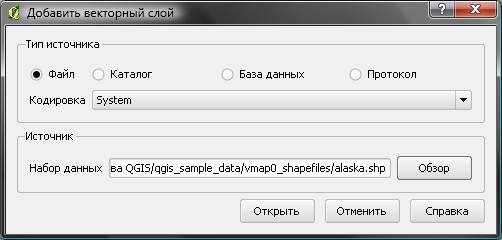
\includegraphics[clip=true, width=12cm]{addvectorlayerdialog}
   \caption{Finestra di dialogo Aggiungi vettore \nixcaption}\label{fig:addvectorlayer}
\end{figure}

\begin{figure}[ht]
   \centering
   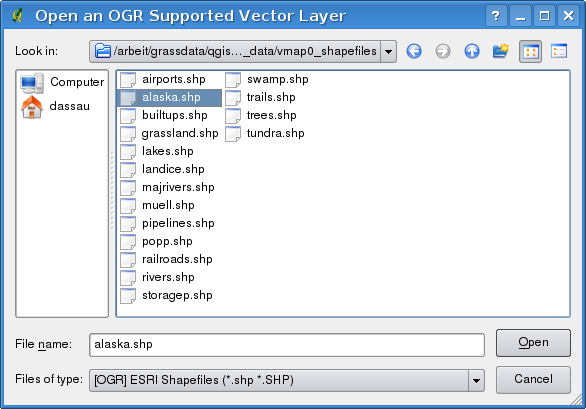
\includegraphics[clip=true, width=12cm]{shapefileopendialog}
   \caption{Finestra di dialogo per aprire un layer vettoriale supportao da OGR \nixcaption}\label{fig:openshapefile}
\end{figure}

\begin{figure}[ht]
   \centering
   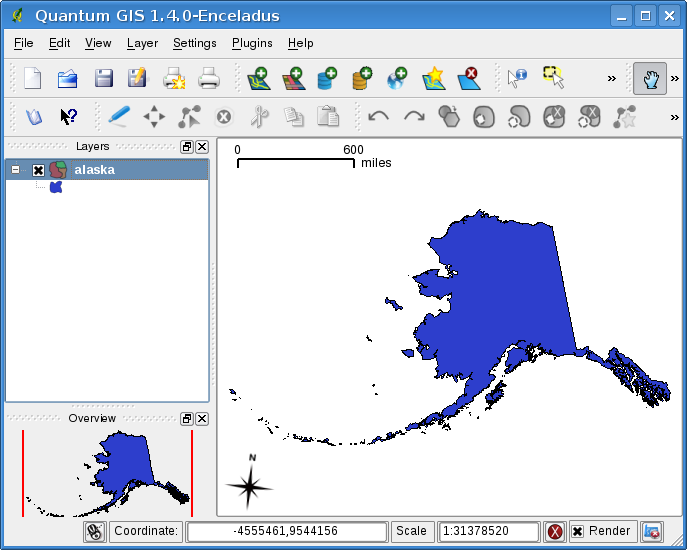
\includegraphics[clip=true, width=12cm]{shapefileloaded}
   \caption{\qg con caricato lo shapefile Alaska \wincaption}\label{fig:loadedshapefile}
\end{figure}

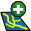
\includegraphics[width=0.7cm]{mActionAddNonDbLayer} 
Per caricare uno shapefile avviare \qg e cliccare sul pulsante
\toolbtntwo{mActionAddNonDbLayer}{Aggiungi vettore}
\index{shapefile!caricamento} o semplicemente digitare \keystroke{Ctrl-Shift-V}.
Nella finestra di dialogo successiva selezionare \radiobuttonon{File}; si aprirà 
una finestra di dialogo standard (Figura \ref{fig:addvectorlayer}) che 
consente di cercare nel filesystem lo shapefile o qualunque altro dato vettoriale 
si intenda caricare. 
La casella di selezione \selectstring{Tipo file}{\ldots} consente di
preselezionare alcuni formati supportati da OGR.

Se lo si desidera, può essere inoltre selezionata la codifica (encoding) da utilizzare
per lo shapefile.

Selezionando uno shapefile dalla lista e cliccando su \button{Open} esso viene
caricato in \qg. La figura \ref{fig:loadedshapefile} mostra come appare
l'interfaccia di \qgis dopo aver caricato il file \filename{alaska.shp}.

\begin{Tip}\caption{\textsc{Colori del layer}}
Quando un layer viene aggiunto alla mappa, gli viene assegnato un
colore a caso. Aggiungendo più layer in una sola volta, ad ognuno di essi
viene assegnato un colore differente.
\end{Tip}

Una volta caricato lo shapefile, si può interagire con la mappa usando 
gli strumenti di navigazione.
Per cambiare la rappresentazione di un layer, aprire la finestra di dialogo
\dialog{Proprietà layer} facendo doppio click sul nome del layer e quindi sulla
scheda Stile o cliccando con il tasto destro sul nome del layer nella legenda 
e scegliendo \dropmenuopt{Proprietà} dal menu contestuale. Si veda la Sezione
\ref{sec:symbology} per ulteriori informazioni su come settare la simbologia
dei layer vettoriali.

\begin{Tip}\caption{\textsc{Caricare layer e progetti da drive esterni in OS X}}
In OS X i drive esterni non vengono elencati come atteso selezionando File 
\arrow Apri progetto. Stiamo lavorando alla creazione di un dialogo apri/salva 
nativo OSX; come soluzione temporanea è possibile digitare '/Volume' nella 
casella Nome file e cliccare invio. Sarà così possibile utilizzare i drive esterni.
\end{Tip}

\subsection{Ottimizzare le prestazioni}

Per migliorare le prestazioni di disegno di uno shapefile, può essere creato
un indice spaziale. Un \index{indice spaziale!shapefile} indice spaziale
migliora la velocità di disegno quando si usano le funzioni di zoom e di
spostamento. Gli indici spaziali usati da \qg hanno estensione \filename{.qix}.

Per creare un indice, seguire queste indicazioni:

\begin{itemize}[label=--]
\item Caricare uno shapefile.
\item Aprire la finestra di dialogo \dialog{Proprietà layer} facendo doppio click
sul nome dello shapefile nella legenda o cliccando su di esso con il tasto
destro e scegliendo la voce \dropmenuopt{Proprietà} dal menu contestuale.
\item Nella scheda \tab{Generale} cliccare sul pulsante \button{Crea indice
spaziale}.
\end{itemize}

\section{Caricare un layer MapInfo}
\index{layer vettoriali!MapInfo}

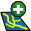
\includegraphics[width=0.7cm]{mActionAddNonDbLayer} Per caricare un layer MapInfo, 
cliccare nella barra strumenti sul pulsante \toolbtntwo{mActionAddNonDbLayer}{Aggiungi vettore} 
o digitare {Ctrl-Shift-V}, cambiare il filtro sul tipo di file nel menu a tendina a
\selectstring{Tipo file}{[OGR] MapInfo (*.mif *.tab *.MIF *.TAB)} e
selezionare il layer che si intende caricare.

\section{Caricare una coverage binaria ArcInfo}
\index{layer vettoriali!coverage ArcInfo}

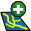
\includegraphics[width=0.7cm]{mActionAddNonDbLayer} Per caricare una coverage binaria
ArcInfo cliccare nella barra strumenti sul pulsante
\toolbtntwo{mActionAddNonDbLayer}{Aggiungi vettore} o digitare
\keystroke{Ctrl-Shift-V} per aprire la finestra di dialogo \dialog{Add Vector 
Layer}. Selezionare \radiobuttonon{Cartella} e \selectstring{Tipo}{Coverage binaria Arc/Info}, 
scorrere il filesystem per individuare la cartella contenente i file della coverage e selezionarla.

Allo stesso modo è possibile caricare file vettoriali strutturati in cartelle nel formato 
di trasferimento UK National Transfer Format o anche nel formato TIGER del US Census Bureau.

\section{Layer PostGIS}
\index{layer vettoriali!PostGIS|vedi{PostGIS}}
\index{PostGIS!layer}
\label{label_postgis} 

I layer PostGIS sono memorizzati in database PostgreSQL. I vantaggi
nell'uso di PostGIS stanno nelle capacità fornite di creazione dell'indice spaziale,
di filtraggio e di interrogazione. Usando PostGIS, le funzioni
vettoriali come la selezione e l'identificazione in \qg lavorano con maggiore
precisione che con i layer OGR.

\subsection{Creare una connessione}\index{PostgreSQL!connessione}\label{sec:postgis_stored}

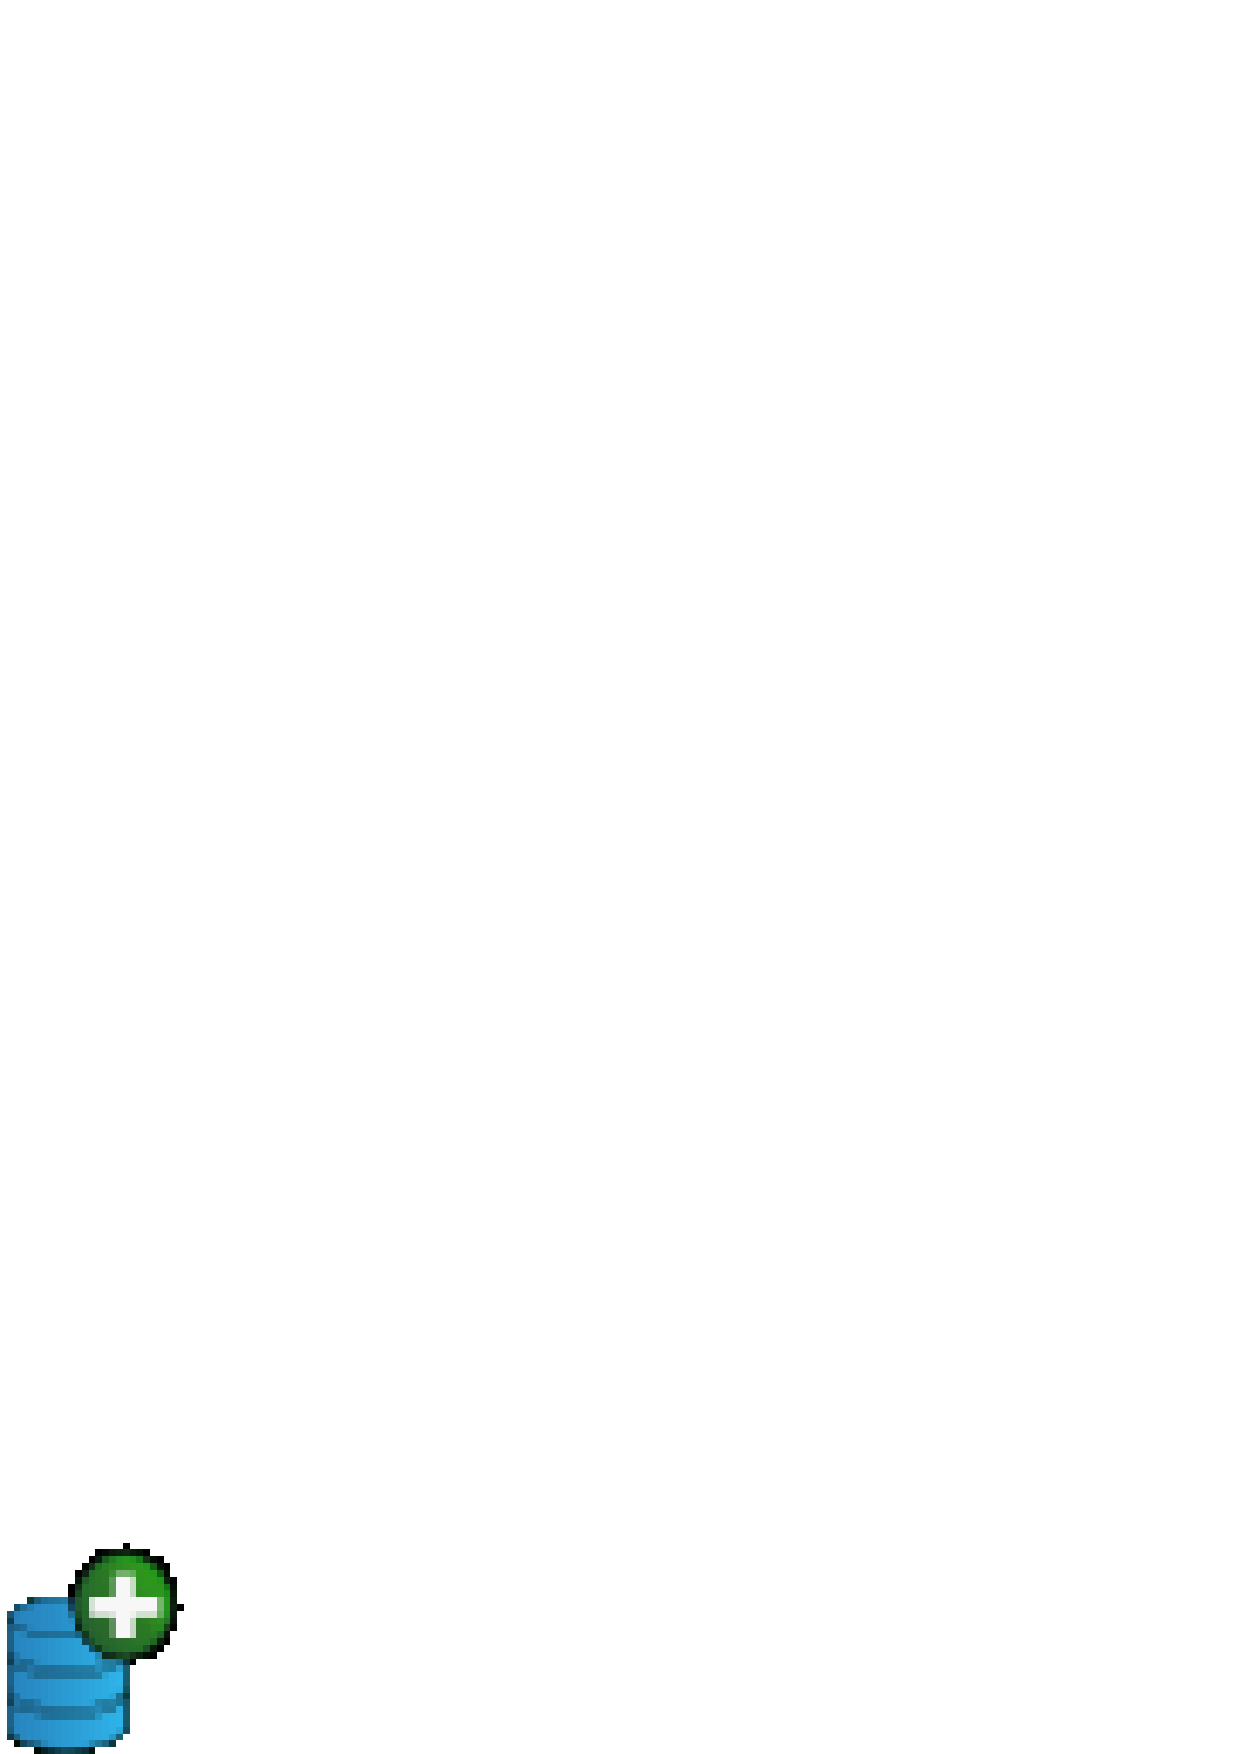
\includegraphics[width=0.7cm]{mActionAddLayer} La prima volta in cui viene
usata una fonte dati PostGIS, bisogna creare una connessione al database
PostgreSQL che contiene i dati. Cliccare nella barra strumenti sul pulsante
\toolbtntwo{mActionAddLayer}{Aggiungi vettore PostGIS} oppure selezionare l'opzione
\dropmenuopttwo{mActionAddLayer}{Aggiungi vettore PostGIS} dal menu
\mainmenuopt{Layer} o digitare \keystroke{Ctrl-Shift-D}. È inoltre possibile 
utilizzare la finestra di dialogo \dialog{Aggiungi vettore} e selezionare 
\radiobuttonon{Database}.
Si aprirà  la finestra di dialogo \dialog{Aggiungi tabella(e) PostGIS}. Per
accedere al gestore della connessione \index{PostgreSQL!gestore della connessione} 
cliccare sul tasto \button{Nuovo} per far comparire la finestra di
dialogo \dialog{Crea una nuova connessione PostGIS}. I parametri richiesti
per la connessione sono mostrati nella tabella \ref{tab:postgis_connection_parms}.

\begin{table}[ht]\index{PostgreSQL!parametri di connessione}
\centering
\caption{Parametri di connessione a PostGIS}\label{tab:postgis_connection_parms}\medskip
 \begin{tabular}{|l|p{5in}|}
\hline Nome & Nome della connessione. Può essere uguale a quello del \textsl{Database}. \\
\hline Servizio & Parametri del servizio da usare alternativamente a host/porta 
(e potenzialmente database). Ciò può essere definito in pg\_service.conf \\
\hline Host \index{PostgreSQL!host}
& Nome del server che ospita il database. Deve essere un host con indirizzo
raggiungibile, lo stesso che potrebbe essere usato per aprire una connessione
telnet o per fare il ping all'host. Se il database è sullo stesso computer sul quale
è installato \qg, inserire semplicemente "localhost". \\
\hline Porta \index{PostgreSQL!porta}& Numero della porta sulla quale il
database PostgreSQL è in ascolto. La porta predefinita è 5432.\\
\hline Database \index{PostgreSQL!database} & Nome del database.  \\
\hline Modalità SSL \index{PostgreSQL!modalità ssl} & Modalità di connessione SSL con il server. 
Le opzione sono:
\begin {itemize}
\item disabilitato: connessione SSL non criptata;
\item permesso: tenta una connessione non SSL, se questa fallisce ne tenta una SSL;
\item preferito: tenta una connessione SSL, se questa fallisce ne prova una non SSL;
\item richiesto: solo connessione SSL.
\end {itemize}
Si noti che è possibile ottenere una notevole velocità di visualizzazione dei layer 
PostGIS disabilitando la connessione SSL. \\
\hline Nome utente \index{PostgreSQL!nome utente}& Nome dell'utente che accede al
database. \\
\hline Password \index{PostgreSQL!password}& Password usata
dall'\textsl{Username} per collegarsi al database.\\
\hline
\end{tabular}
\end{table}

Come opzione, possono essere attivate le seguenti caselle di controllo:

\begin{itemize}[label=--]
\item \checkbox{Salva nome utente}
\item \checkbox{Salva Password}
\item \checkbox{Cercare solamente nella tabella geometry\_columns}
\item \checkbox{Cerca solamente nello schema}
\item \checkbox{Mostra anche tabelle senza geometria}
\item \checkbox{Usa i metadati stimati della tabella}
\end{itemize}

Quando tutti i parametri sono impostati, la connessione può essere testata
cliccando sul pulsante \button{Test connessione} \index{PostgreSQL!connessione!test}.

\begin{Tip}\caption{\textsc{Impostazioni utente e Sicurezza}}\index{impostazioni}\index{sicurezza}
Le impostazioni personalizzate di \qg sono salvate in modo diverso
in base al sistema operativo. \nix, le impostazioni sono salvate nella
cartella home dell'utente nel file \filename{.\qg}. \win, le
impostazioni sono salvate nel registro di sistema. Secondo il sistema
operativo, il salvataggio delle password in \qg può essere più o meno rischioso.
\end{Tip}

\subsection{Caricare un layer PostGIS}\index{PostgreSQL!caricamento layer}

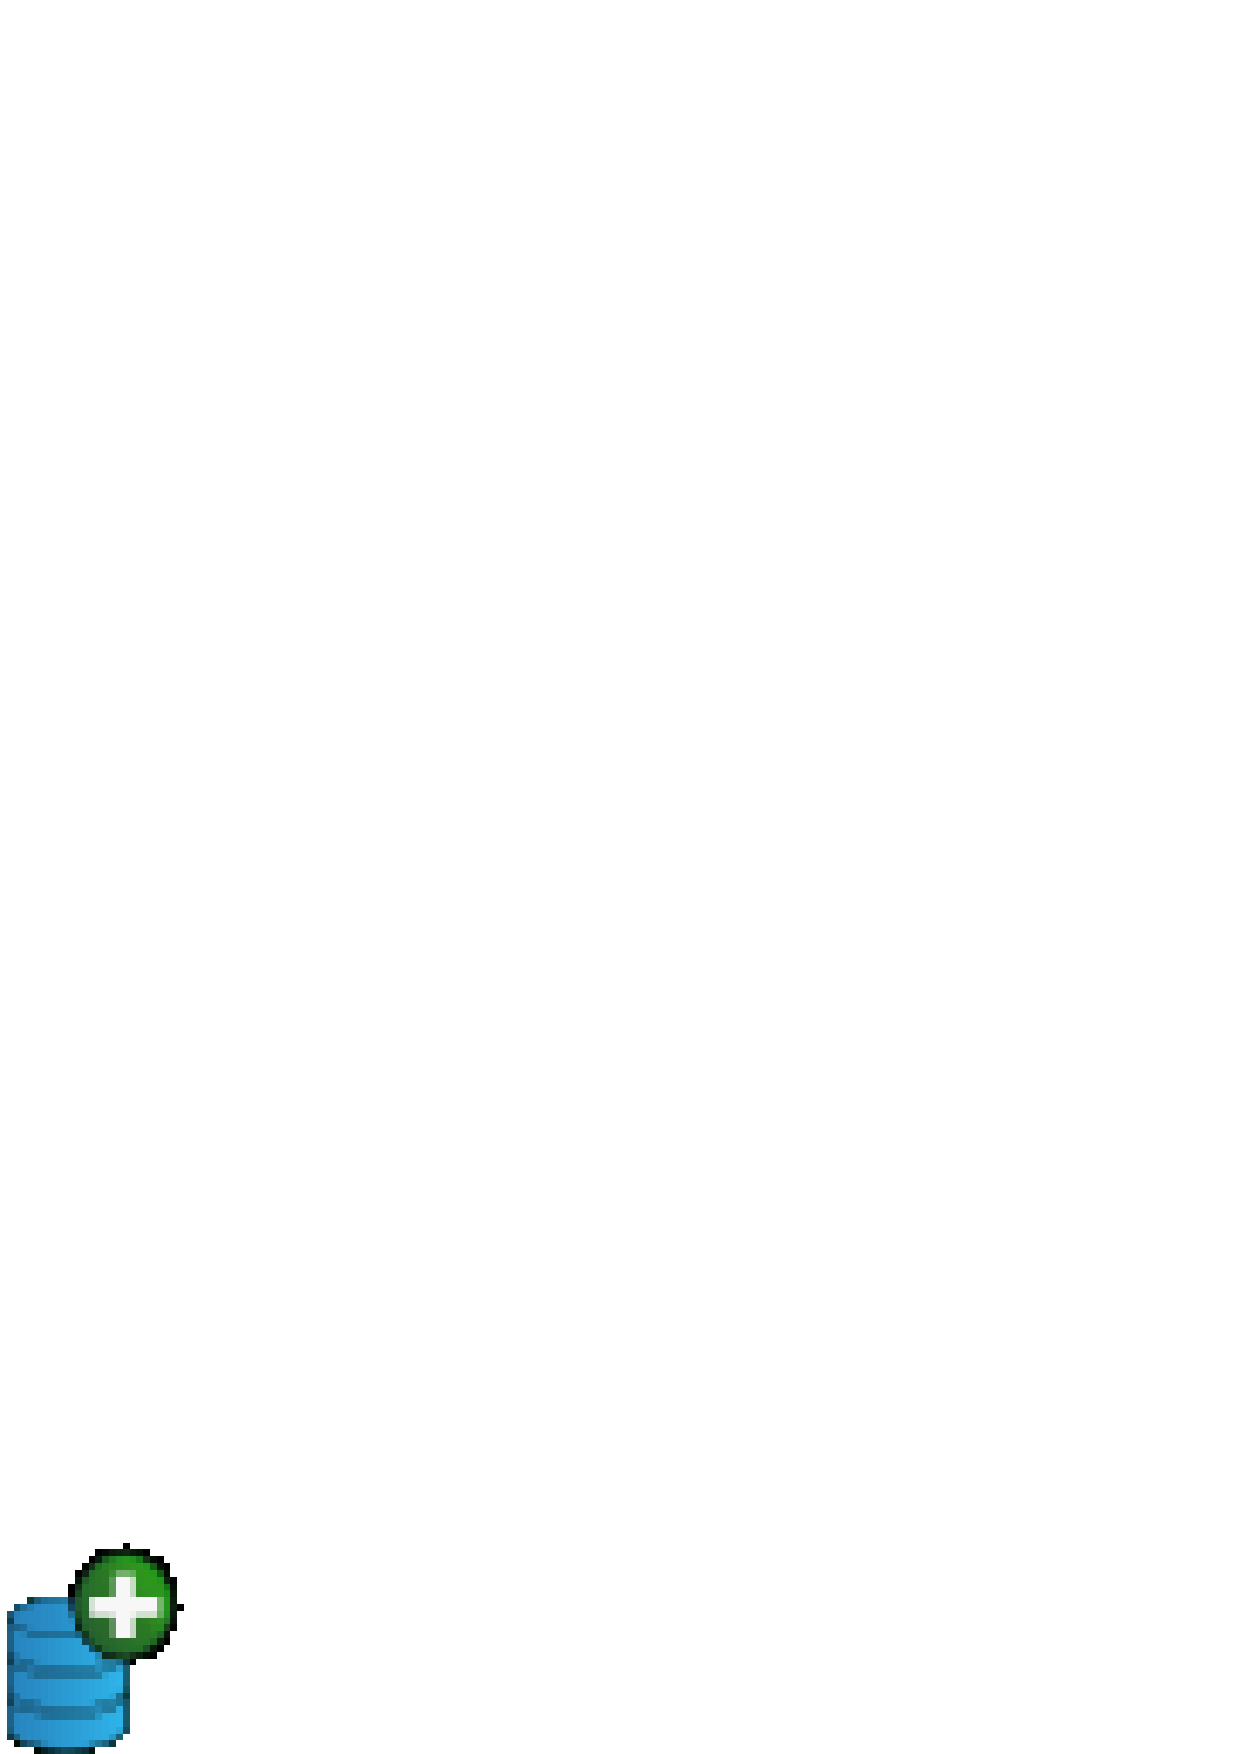
\includegraphics[width=0.7cm]{mActionAddLayer} Una volta definita una 
connessione, si possono caricare layer dal database PostgreSQL.
Ovviamente questo richiede avere dati in PostgreSQL. Si veda la Sezione
\ref{sec:loading_postgis_data} per informazioni sul come importare dati nel
database. 

Per caricare layer da PostGIS, seguire i seguenti passaggi:

\begin{itemize}[label=--]
\item Se la finestra di dialogo \dialog{Aggiungi tabella(e) PostGIS} non è già
aperta, cliccare nella barra strumenti sul pulsante
 \toolbtntwo{mActionAddLayer}{Aggiungi vettore PostGIS}.
\item Scegliere la connessione dal menu a tendina e cliccare su \button{Connetti}.
\item Selezionare/deselezionare \checkbox{Mostra tabelle senza geometria}
\item Opzionalmente usare \checkbox{Opzioni ricerca} per definire quali elementi 
caricare dal layer oppure utilizzare \button{Crea query} per avviare la finestra 
di dialogo Query builder.
\item Individuare il layer che si vuole aggiungere nella lista di quelli disponibili.
\item Selezionare il layer cliccando sul nome. È possibile selezionare più layer
tenendo premuto il tasto \keystroke{shift} mentre si seleziona. Si veda la
Sezione \ref{sec:query_builder} per informazioni su come usare il Query builder 
PostgreSQL per definire una selezione al momento del caricamento.
\item Cliccare sul tasto \button{Aggiungi} per aggiungere il layer alla mappa.
\end{itemize}

\begin{Tip}\caption{\textsc{layer PostGIS}}
Di solito un layer PostGIS è definito da un record nella tabella
geometry\_columns. Dalla versione \OLD % should be 0.9.0 
in avanti, \qg può caricare layer che non hanno tale record nella tabella
geometry\_columns. Ciò vale sia per le tabelle che per le viste. La
definizione di una vista spaziale fornisce un mezzo molto potente per
visualizzare i dati. Fare riferimento al manuale PostgreSQL per informazioni
su come creare le viste.
\end{Tip}

\subsection{Alcuni dettagli sui layer PostgreSQL}\label{sec:postgis_details}
\index{PostgreSQL!dettagli layer}

Questa sezione contiene alcuni dettagli su come \qg accede ai layer
PostgreSQL. La maggior parte delle volte \qg dovrebbe semplicemente fornire
una lista di tabelle del database che possono essere caricate e caricarle su
richiesta. Tuttavia, se avete difficoltà a caricare una tabella di PostgreSQL
in \qg, le informazioni seguenti possono aiutare a capire tutti i messaggi 
di \qg ed a dare un'indicazione su come cambiare la definizione di tabella o 
di vista di PostgreSQL per permettere a \qg di caricarla.

\qg richiede che i layer di PostgreSQL contengano una colonna che possa essere usata come
chiave unica per il layer. Per le tabelle questo significa che esse devono
contenere una chiave primaria o una colonna con un vincolo unico. 
Se una tabella manca di questi elementi, verrà usata la colonna 'oid'. 
\qg richiede che questa colonna sia di tipo int4 (un numero intero di 4 byte). 
Le prestazioni saranno migliori se la colonna è indicizzata (notare che le 
chiavi primarie sono automaticamente indicizzate in PostgreSQL).

Se il layer di PostgreSQL è una vista, esistono gli stessi requisiti, ma le
viste non hanno chiavi primarie o colonne con i vincoli unici su di loro. In
questo caso \qg proverà a trovare una colonna nella vista che provenga 
da una colonna appropriata della tabella. Ciò viene fatto analizzando la 
definizione SQL della vista; ci sono diversi aspetti di SQL che sono ignorati da \qg 
(es. l'uso di alias di tabelle e colonne generate da funzioni SQL).

Se non viene trovata alcuna colonna adatta, \qg non caricherà il layer. 
Se questo accade, la soluzione è di alterare la vista in modo che includa una 
colonna adatta (di tipo int4 e una chiave primaria o un vincolo unico, 
preferibilmente indicizzato).

\subsection{Importare dati in PostgreSQL}\label{sec:loading_postgis_data}
\index{PostGIS!SPIT!importare dati}

\minisec{shp2pgsql}
I dati possono essere importati in PostgreSQL in diverse maniere. PostGIS
include un programma di utilità chiamato \filename{shp2pgsql} che può essere
usato per importare shapefile in un database PostGIS. Per esempio, per
importare lo shapefile chiamato \filename{lakes.shp}
nel database PostgreSQL chiamato \usertext{gis\_data}, usare il comando
seguente:

\begin{verbatim} 
  shp2pgsql -s 2964 lakes.shp lakes_new | psql gis_data
\end{verbatim}

Questo comando crea un nuovo layer chiamato \usertext{lakes\_new} nel database
\usertext{gis\_data}. Il nuovo layer avrà un identificatore di riferimento 
spaziale (Spatial Reference Identifier - SRID) di 2964. 
Si veda la Sezione \ref{label_projections} per ulteriori informazioni
sui sistemi di riferimento spaziale e le proiezioni.
\begin{Tip}
\caption{\textsc{Esportare dati da PostGIS}\index{PostGIS!esportazione}}
Oltre allo strumento per l'importazione \filename{shp2pgsql}, esiste uno 
strumento per l'esportazione di dati PostGIS come shapefile:
\filename{pgsql2shp}. Lo strumento è incluso nella versione di PostGIS corrente.
\end{Tip}

\minisec{Plugin SPIT}

\includegraphics[width=0.7cm]{spiticon} \qg include un plugin denominato SPIT 
(Shapefile to PostGIS Import Tool)\index{PostGIS!SPIT}.
SPIT può essere usato per caricare più shapefile contemporaneamente e
include il supporto per gli schemi. Per usare SPIT, aprire il gestore dei plugin
dal menu \mainmenuopt{Plugins}, selezionare la casella di controllo vicina a
\checkbox{SPIT} e cliccare su \button{OK}. L'icona di SPIT verrà aggiunta alla
barra degli strumenti plugin\index{PostGIS!SPIT!caricamento}. 

Per importare uno shapefile, cliccare sull'icona \toolbtntwo{spiticon}{SPIT} 
nella barra degli strumenti per aprire la finestra di dialogo \\
\dialog{SPIT - Shapefile to PostGIS Import Tool}. Selezionare il database 
PostGIS al quale si desidera connettersi e cliccare su \button{Connetti}.
Ora è possibile aggiungere uno o più file alla coda cliccando su \button{Aggiungi}. 
Per processare i file selezionati, cliccare su \button{OK}. L'avanzamento 
dell'importazione ed eventuali errori/avvertimenti saranno mostrati mentre 
ciascuno shapefile viene elaborato.

\begin{Tip}\caption{\textsc{Importare shapefile contenenti parole riservate 
in PostgreSQL}}\index{PostGIS!SPIT!parole riservate}
Se alla coda d'importazione viene aggiunto uno shapefile contenente campi 
con parole riservate per il database PostgreSQL, comparirà una finestra di dialogo
che darà informazioni sullo stato di ogni campo. È necessario modificare i nomi
dei campi contenenti tali parole (ed è possibile eventualmente editare anche
il nome degli altri campi) \index{PostGIS!SPIT!editare il nome dei campi}
prima dell'importazione, altrimenti il processo di importazione non
andrà a buon fine.
\end{Tip} 

\minisec{ogr2ogr}
Oltre a \filename{shp2pgsql} e \filename{SPIT} c'è un altro strumento per
caricare dati in PostGIS: \filename{ogr2ogr}. \\
\filename{ogr2ogr} fa parte della versione di GDAL installata..
Per importare uno shapefile in PostGIS con \filename{ogr2ogr}, digitare il 
seguente comando:
\begin{verbatim}
  ogr2ogr -f "PostgreSQL" PG:"dbname=postgis host=myhost.de user=postgres \
  password=topsecret" alaska.shp
\end{verbatim}

L'espressione importerà lo shapefile \filename{alaska.shp} nel database PostGIS
\usertext{postgis}
usando l'utente \usertext{postgres} e la password \usertext{topsecret} sull'host
\server{myhost.it}.

Notare che OGR deve essere compilato con il supporto a PostgreSQL per poter
effettuare tale operazione.
La presenza del supporto a PostgreSQL-PostGIS può essere verificata digitando
da riga di comando:
\begin{verbatim}
ogrinfo --formats | grep -i post
\end{verbatim}

Qualora si volesse usare il comando interno di PostgreSQL \filename{COPY} al posto
del metodo predefinito \filename{INSERT INTO}, bisogna settare le variabili
d'ambiente come segue (su piattaforme \nix e \osx):
\begin{verbatim}
  export PG_USE_COPY=YES
\end{verbatim}

\filename{ogr2ogr} non crea indici spaziali come \filename{shp2pgsl}. Bisogna
crearli manualmente, usando il comando SQL \filename{CREATE INDEX} dopo
l'importazione, come passaggio aggiuntivo (Sezione \ref{label_improve}).

\subsection{Migliorare le prestazioni} \label{label_improve}

Richiamare dati geografici da un database PostgreSQL può richiedere molto
tempo, specialmente se il server dei dati si trova in rete. È possibile
migliorare le prestazioni di resa a video di layer PostgreSQL assicurandosi
di creare un \index{PostGIS!indice spaziale} indice spaziale su ogni layer nel
database. PostGIS supporta la creazione di un \index{PostGIS!indice
spaziale!GiST} indice GiST
(indice dell'albero generalizzato di ricerca, Generalized Search Tree) per
velocizzare le ricerche spaziali di dati.

La sintassi per la creazione di un indice GiST è:
\footnote{le informazioni sull'indice GiST
sono tratte dalla documentazione PostGIS disponibile su \url{http://postgis.refractions.net}}

\begin{verbatim}
    CREATE INDEX [indexname] ON [tablename] 
      USING GIST ( [geometryfield] GIST_GEOMETRY_OPS );
\end{verbatim}

Si noti che per tabelle molto grandi, la creazione dell'indice può richiedere
parecchio tempo. Non appena l'indice è stato creato, bisognerebbe effettuare
un \usertext{VACUUM ANALYZE}. Si veda la documentazione di PostGIS
\cite{PostGISweb} per ulteriori informazioni.

Segue un esempio di come creare un indice GiST:
\begin{verbatim}
gsherman@madison:~/current$ psql gis_data
Welcome to psql 8.3.0, the PostgreSQL interactive terminal.

Type:  \copyright for distribution terms
        \h for help with SQL commands
        \? for help with psql commands
        \g or terminate with semicolon to execute query
        \q to quit

gis_data=# CREATE INDEX sidx_alaska_lakes ON alaska_lakes
gis_data-# USING GIST (the_geom GIST_GEOMETRY_OPS);
CREATE INDEX
gis_data=# VACUUM ANALYZE alaska_lakes;
VACUUM
gis_data=# \q
gsherman@madison:~/current$
\end{verbatim}

\subsection{Layer vettoriali a cavallo dei 180$^\circ$ di longitudine}
\index{vector layers!180 gradi}

Molti software GIS non gestiscono appropriatamente le mappe vettoriali, con 
sistema di riferimento geografico (lat/lon), a cavallo della linea di longitudine \degrees{180}. 
Se si apre una di tali mappe in \qg vedremmo distanti aree geografiche che sono in realtà 
vicine tra di loro.

Nella figura \ref{fig:vector_not_wrapping} il piccolo punto all'estrema sinistra 
della vista mappa (Chatham Islands) dovrebbe essere all'interno della griglia subito 
alla destra dell'isola principale della Nuova Zelanda.

\begin{figure}[ht]
   \centering
   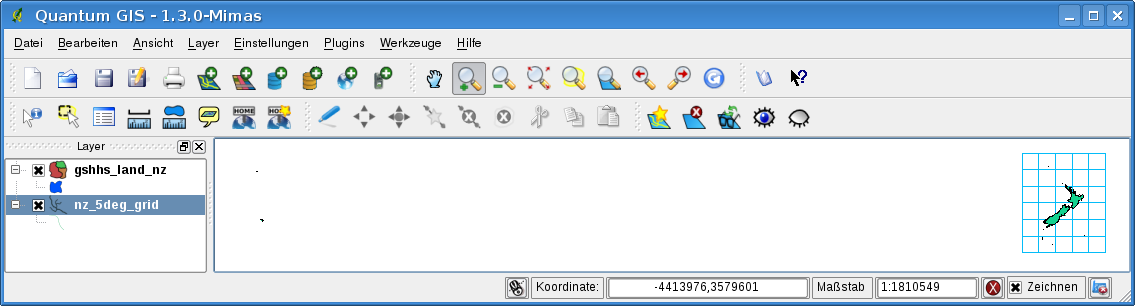
\includegraphics[clip=true, width=\textwidth]{vectorNotWrapping}
      \caption{Mappa in lat/lon a cavallo della linea di longitudine \degrees{180} \nixcaption}
   \label{fig:vector_not_wrapping}
\end{figure}

Come soluzione è possibile trasformare i valori di longitudine utilizzando PostGIS 
e la funzione \textbf{ST\textunderscore Shift\textunderscore Longitude}
\footnote{\url{http://postgis.refractions.net/documentation/manual-1.4/ST\_Shift\_Longitude.html}}. 
La funzione legge ogni punto/vertice di ogni elemento in una geometria e se la coordinata di 
longitudine è < \degrees{0}, gli aggiunge \degrees{360}. 
Il risultato sarà una versione \degrees{0} - \degrees{360} dei dati, che verranno poi 
tracciati su una mappa centrata a \degrees{180}.

\begin{figure}[ht]
   \centering
   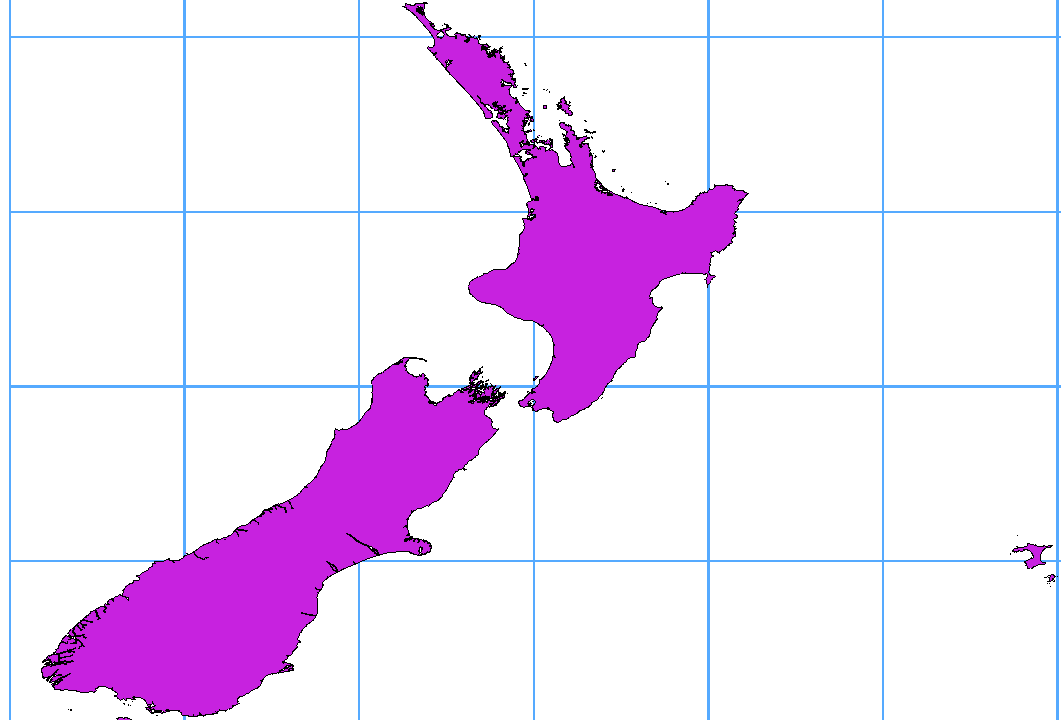
\includegraphics[clip=true, width=9cm]{vectorWrapping}
   \caption{Mappa a cavallo della linea di longitudine \degrees{180} dopo l'utilizzo della funzione ST\textunderscore 
   Shift\textunderscore Longitude \nixcaption}
\label{fig:vector_wrapping}
\end{figure}

\minisec{Guida all'uso}

\begin{itemize}[label=--]
\item Importare i dati in PostGIS (\ref{sec:loading_postgis_data}) utilizzando 
per esempio SPIT
\item Utilizzare l'interfaccia da linea di comando di PostGIS per dare il seguente comando
(nell'esempio "TABLE" è il nome della tabella PostGIS) \\
\texttt{gis\_data=\# update TABLE set the\_geom=ST\_shift\_longitude(the\_geom);}
\item Se il comando ha esito positivo, si riceverà una notifica di conferma circa il 
numero di elementi aggiornati e sarà possibile caricare i dati (Figura \ref{fig:vector_wrapping}).
\end{itemize}

\section{Layer SpatiaLite}
\index{Layer SpatiaLite!proprietà}
\index{layer vettoriali!SpatlaLIte|vedi{SpatiaLite}}
\index{SpatiaLite!layer}
\label{label_spatialite}

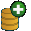
\includegraphics[width=0.7cm]{mActionAddSpatiaLiteLayer}
Per caricare dei dati da un database SpatiaLite cliccare sullo strumento 
\toolbtntwo{mActionAddSpatiaLiteLayer}{Aggiungi un layer SpatiaLite} o selezionare 
l'opzione \dropmenuopttwo{mActionAddSpatiaLiteLayer}{Aggiungi un layer SpatiaLite} 
dal menu \mainmenuopt{Layer} oppure digitare \keystroke{Ctrl+Shift+L}.
Si aprirà una finestra di dialogo che permette di accedere ai dati di un database 
SpatiaLite già connesso a \qg oppure di definire la connessione ad un nuovo 
database: per connettersi ad un nuovo database cliccare su \button{Nuovo} e selezionare 
il database SpatiaLite, un file con estensione \filename{.sqlite }.

Per salvare, invece, un layer vettoriale in formato SpatialLite, cliccare con il tasto 
destro del mouse sul layer nella legenda e selezionare l'opzione \dropmenuopt{Salva con nome...}, 
definire il nome del file in uscita, selezionare SQLite con formato e il SR, aggiungere 
'SPATIALITE=YES' nel riquadro Sorgente dati delle opzioni di creazione OGR. Si veda inoltre
\url{http://www.gdal.org/ogr/drv_sqlite.html}.

\minisec{Creare un nuovo layer SpatiaLite}

Per creare un nuovo layer SpatiaLite, riferirsi alla Sezione \ref{sec:create spatialite}.

\begin{Tip}\caption{\textsc{SpatiaLite data management Plugin}}\index{SpatiaLite!gestione dati} 
Per la gestione dei dati SpatiaLite è inoltre possibile utilizzare il plugin 'QspatiaLite' disponibile 
tra i repositori di terze parti dell'Installatore \qg Python Plugin. QspatiaLite permette di 
importare layer, visualizzare tabelle e query spaziali in \qg e fornisce un editor SQL 
con funzionalità di evidenziazione della sintassi e di autocompletamento, oltre ad un 
costruttore di query ed altre funzionalità. 
\end{Tip}

\section{Proprietà dei layer vettoriali}\label{sec:vectorprops}
\index{layer vettoriali!finestra delle proprietà}

La finestra di dialogo \dialog{Proprietà layer} fornisce informazioni
sul layer, sulla sua rappresentazione grafica (stile) e sulle opzioni di
visualizzazione delle etichette. Inoltre, se il layer vettoriale è stato caricato 
da un archivio dati PostgreSQL/PostGIS, è possibile modificare l'espressione 
SQL che lo ha generato tramite la finestra di dialogo \dialog{Query builder} 
nella scheda \tab{Generale}. 
Per accedere alla finestra di dialogo \dialog{Proprietà layer}, fare
doppio click sul layer nella legenda o click con il tasto destro sul layer e
selezionare \dropmenuopt{Proprietà} dal menu contestuale.

\begin{figure}[ht]
   \centering
   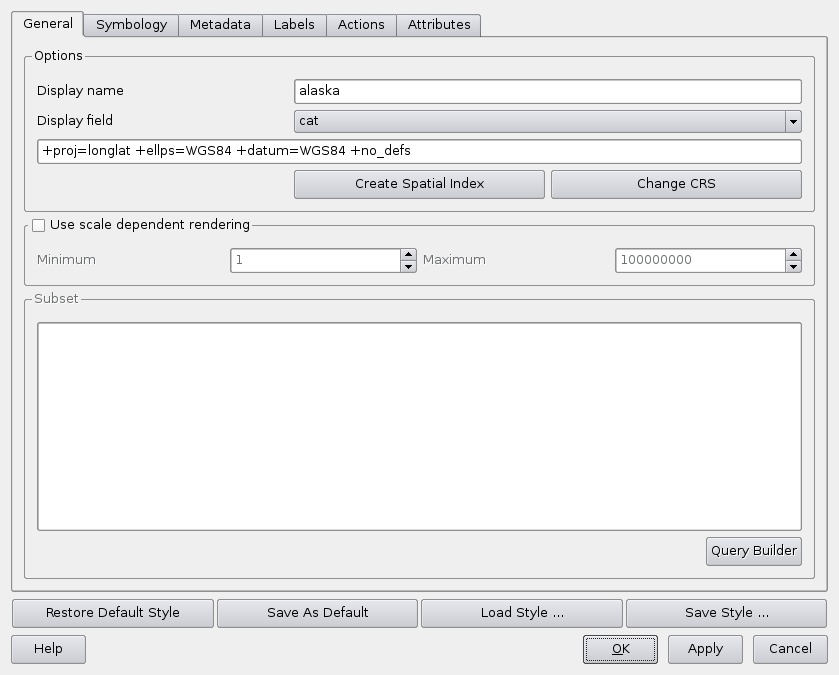
\includegraphics[clip=true, width=12cm]{vectorLayerSymbology}
   \caption{Finestra di dialogo delle proprietà di un vettore \nixcaption}\label{fig:vector_symbology}
 \end{figure}

\subsection{Scheda Stile}\label{sec:symbology}
\index{layer vettoriali!stile}

A partire dalla versione 1.4.0 \qg utilizza una nuova simbologia per migliorare e in prospettiva 
sostituire la vecchia simbologia. \qg 1.7.0 utilizza in modalità predefinita la nuova simbologia: 
questa fornisce diversi miglioramenti e nuove funzionalità.

Una descrizione della vecchia simbologia è disponibile nella Sezione \ref{sec:oldsymbology}.

\minisec{Comprendere la simbologia di nuova generazione}

La nuova simbologia utilizza tre tipi di simboli: indicatore (per i punti), linea (per le linee) 
e riempimento (per i poligoni). I simboli possono consistere di uno o più layer 
simbolo. È possibile impostare il colore di un simbolo e tale colore sarà poi assegnato a 
tutti i layer simbolo. Alcuni layer possono avere il colore non modificabile; ciò è utile 
quando si imposta il colore per un simbolo multi-layer. Allo stesso modo, è possibile impostare 
lo spessore per i simboli linea e la dimensione e la rotazione dei simboli indicatore.
 
\minisec{Tipi di layer simbolo}

\begin{itemize}[label=--]
\item Layer di punti
\begin{itemize}[label=--]
\item \textbf{Indicatore carattere}: visualizzazione tramite caratteri.
\item \textbf{Indicatore semplice}: visualizzazione tramite indicatori hard-coded.
\item \textbf{Indicatore SVG}: visualizzazione tramite immagini SVG.
\end{itemize}
\item Layer di linee 
\begin{itemize}[label=--]
\item \textbf{Decorazione linea}: aggiunge una decorazione alla linea (es. una freccia per indicare la direzione).
\item \textbf{Linea di evidenziazione}: una linea visualizzata tramite la ripetizione di simboli indicatore.
\item \textbf{Linea semplice}: visualizzazione tipica con spessore, colore e stile del tratto.
\end{itemize}
\item Layer di poligoni
\begin{itemize}[label=--]
\item \textbf{Riempimento con centroide}: visualizza un indicatore semplice sul centroide.
\item \textbf{Riempimento SVG}: campisce un poligono con un simbolo SVG. 
\item \textbf{Riempimento semplice}: campitura tipica con colore, stile e bordo.
\item \textbf{Cornice: Decorazione linea}: aggiunge una decorazione alle linee (es. una freccia per indicare la direzione).
\item \textbf{Cornice: Linea di evidenziazione}: usa un indicatore hard-coded come bordo di un'area.
\item \textbf{Cornice: Linea semplice}: definisce spessore, colore e stile del tratto per il bordo di un'area.
\end{itemize}
\end{itemize}

\minisec{Scala di colori}

Le scale di colori servono a definire il range di colori usati dai visualizzatori (Tipo legenda nella vecchia simbologia).
Il colore del simbolo sarà definito in funzione della scala di colori.

Ci sono tre tipi di scale di colori:

\begin{itemize}[label=--]
\item \textbf{Gradiente}: gradiente lineare.
\item \textbf{Casuale}: generazione casuale di colori da un'area specifica dello spazio dei colori.
\item \textbf{ColorBrewer}: utilizza uno schema di colori ed un numero definito di classi di colore.
\end{itemize}

Le scale di colori possono essere create nella scheda \tab{Scala di colori} della finestra di dialogo \dialog{Gestore stile} 
(Sezione \ref{subsec:stylemanager}), cliccando su \button{Aggiungi}.

\minisec{Stili}

Uno stile raggruppa un insieme di vari simboli e scale di colori. È possibile 
definire dei simboli personalizzati ed utilizzarli senza doverli ricreare ogni volta. 
Gli elementi (simboli e scale di colori) di uno stile hanno sempre associato un nome 
che ne facilita la ricerca e la gestione. 
In \qg è presente almeno uno stile predefinito (modificabile) e l'utente può crearne dei nuovi.

\minisec{Visualizzatori}

Un visualizzatore è responsabile della rappresentazione di un elemento con un simbolo. 
Ci sono quattro tipi di visualizzatori: simbolo singolo, categorizzato 
(colore unico nelle vecchia simbologia), graduato e tramite regole. Non è presente 
un visualizzatore di colore continuo in quanto esso è semplicemente un caso speciale 
del visualizzatore graduato. I visualizzatori categorizzato e graduato sono definiti 
specificando un simbolo ed una scala di colori.

\subsection{Lavorare con la simbologia di nuova generazione}\label{new_generation_sym}

Nella scheda \tab{Stile} è possibile selezionare uno dei quattro visualizzatori citati. 
In funzione del visualizzatore scelto, vengono mostrate le impostazioni e le opzioni differenti, 
di seguito descritte.
Nella finestra di dialogo della nuova simbologia il pulsante \button{Gestore di stili...} 
permette di accedere al Gestore stile (Sezione \ref{subsec:stylemanager}). Il Gestore stile permette 
di modificare, creare, eliminare simboli. 

\minisec{Visualizzatore Simbolo singolo}

Il visualizzatore Simbolo singolo rappresenta tutti gli elementi di un layer 
tramite un unico simbolo definito dall'utente. Le diverse opzioni della scheda \tab{Stile} 
variano in funzione tipo di layer, ma tutti i tipi condividono la seguente struttura. 
Nella parte in alto a sinistra della scheda è presente un'anteprima del simbolo. Nella 
parte inferiore è presente una lista di simboli già definiti per lo stile in uso. 
Il simbolo può essere modificato cliccando su \button{Cambia...} sotto l'anteprima, 
che apre la finestra di dialogo \dialog{Proprietà simbolo}, oppure cliccando su \button{Cambia} 
a destra dell'anteprima, che apre la finestra di dialogo \dialog{Select color}. 

Nella scheda \tab{Stile} è possibile impostare la trasparenza e le unità (millimetri o unità 
di mappa) per la dimensione della scala; è inoltre possibile utilizzare una dimensione della 
scala in funzione dei dati e la rotazione (pulsante \button{Avanzato} vicino a \button{Salva come stile}). 
Il pulsante \button{Livelli simbolo} permette di abilitare e definire l'ordine in cui i layer di simboli 
sono visualizzati (se i simboli consistono di più di un layer).

Fatte tutte le modifiche di interesse, il simbolo può essere aggiunto alla lista degli Stili salvati 
(tramite il pulsante \button{Salva come stile}) e riutilizzato successivamente.

\begin{figure}[ht]
\centering
   \subfloat[Proprietà Simbolo singolo punto] {\label{subfig:singleNG1}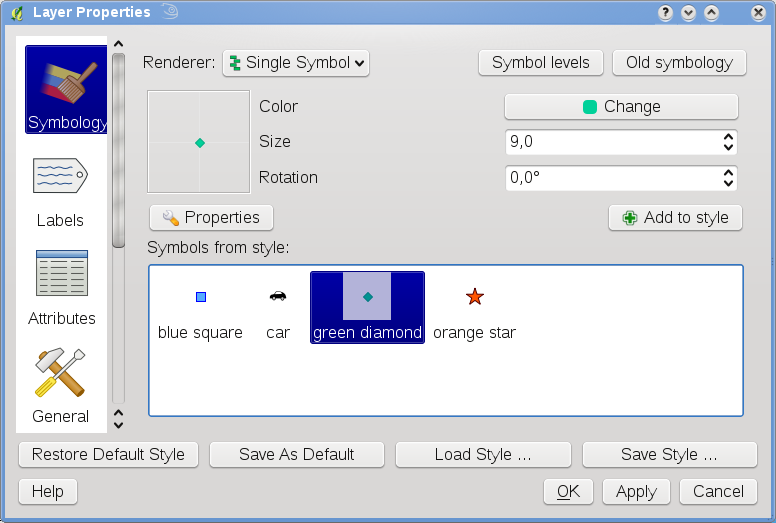
\includegraphics[clip=true, width=0.3\textwidth]{singlesymbol_ng_point}}
   \hspace{1cm}
   \subfloat[Proprietà Simbolo singolo linea] {\label{subfig:singleNG2}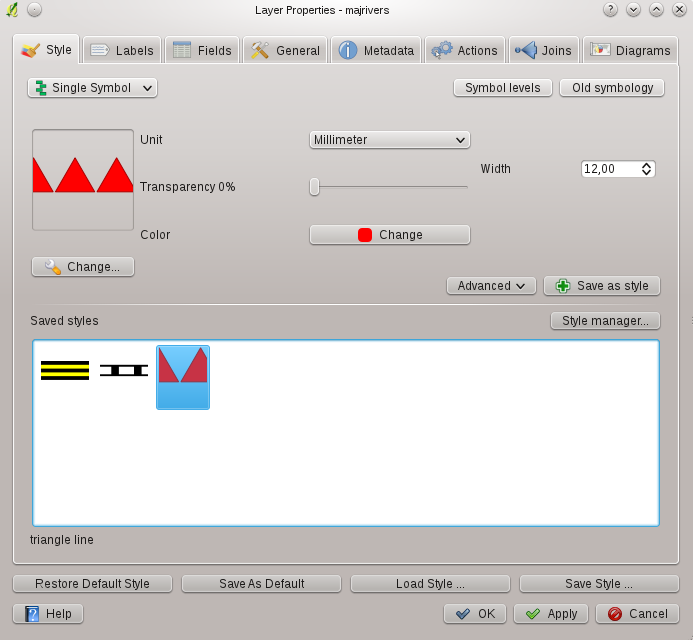
\includegraphics[clip=true, width=0.3\textwidth]{singlesymbol_ng_line}}
   \hspace{1cm}
   \subfloat[Proprietà Simbolo singolo poligono] {\label{subfig:singleNG3}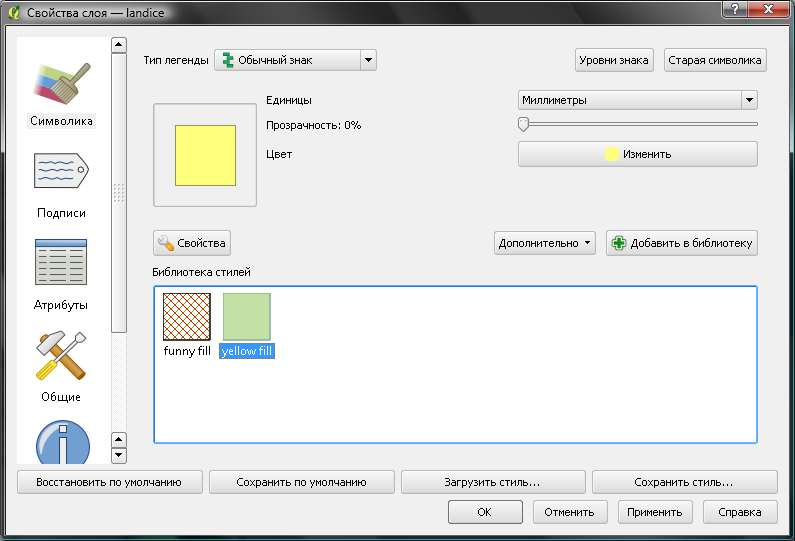
\includegraphics[clip=true, width=0.3\textwidth]{singlesymbol_ng_area}}
\caption{Opzioni di visualizzazione per Simbolo singolo \wincaption}
\end{figure}

\minisec{Visualizzatore Categorizzato}

Il visualizzatore Categorizzato rappresenta tutti gli elementi di un layer 
tramite un unico simbolo definito dall'utente, con i colori che riflettono 
il valore di un attributo specifico. La scheda \tab{Stile} permette di selezionare:

\begin{itemize}[label=--]
\item L'attributo (Colonna)
\item Il simbolo (Simbolo)
\item Il colore (Scala di colori)
\end{itemize}

Con il pulsante \button{Avanzato}, in basso a destra, è possibile impostare il campo di rotazione 
e il campo di dimensione della scala.
Cliccando su \button{Classifica}, in basso a sinistra del riquadro al centro della scheda, 
sarà elencato l'attributo selezionato ed i simboli con cui verranno rappresentati i suoi valori.

L'esempio in figura \ref{fig:catsymNG} mostra la finestra di dialogo per la visualizzazione 
categorizzata del layer rivers dei dati campione di \qg.

\begin{figure}[ht]
   \centering
   \caption{Opzioni di visualizzazione per Simbolo Categorizzato \wincaption}\label{fig:catsymNG}
   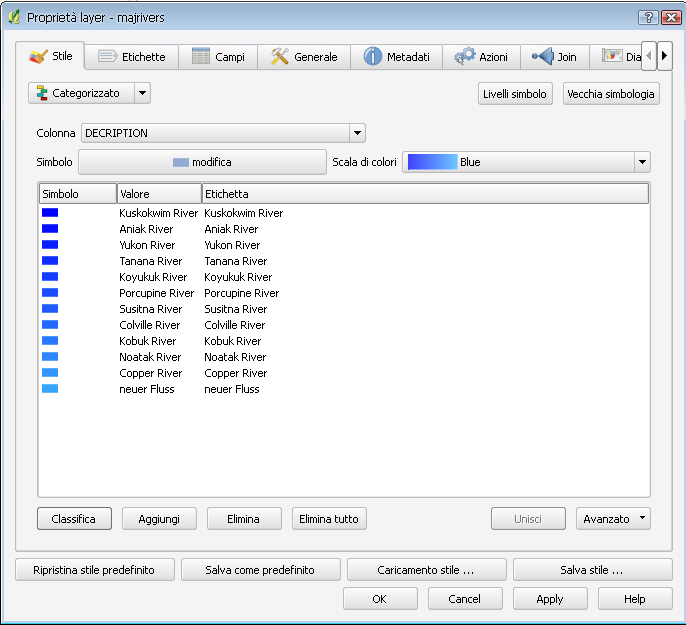
\includegraphics[clip=true, width=10cm]{categorysymbol_ng_line}
\end{figure}

È possibile creare una scala di colori personalizzata selezionando 'Nuova scala di colori...' 
dal menu a discesa Scala di colori. Si aprirà la finestra di dialogo 'Tipo di scala di colori', con 
le opzioni: Gradiente, Casuale, ColorBrewer. Una volta selezionato il tipo, la finestra successiva permette 
di impostare le varie opzioni della scala di colori. Si veda \ref{fig:ccrg} per un esempio di una scala 
di colori personalizzata.

\begin{figure}[ht]
   \centering
   \caption{Esempio di scala di colori a gradiente con interruzioni multiple \wincaption}\label{fig:ccrg}
   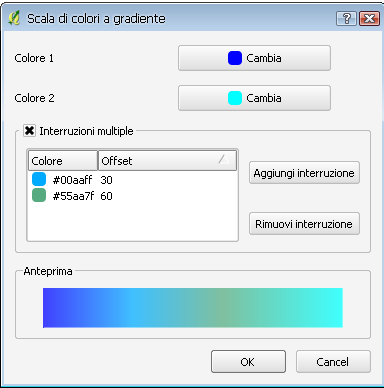
\includegraphics[clip=true, width=6cm]{customColorRampGradient}
\end{figure}

\minisec{Visualizzatore Graduato}

Il visualizzatore Graduato rappresenta tutti gli elementi di un layer 
tramite un unico simbolo definito dall'utente, con i colori che riflettono 
la classificazione di un attributo di interesse. Come il Visualizzatore Simbolo 
categorizzato, permette di impostare la rotazione e la dimensione della scala in 
base a campi specifici.
 
La scheda \tab{Stile} permette di selezionare:

\begin{itemize}[label=--]
\item L'attributo (Colonna)
\item Il simbolo (Simbolo)
\item I colori (Scala di colori)
\end{itemize}

Inoltre, è possibile specificare il numero di classi (Classi) ed il tipo di classificazione 
(Modo). Sono disponibili i seguenti tipi di classificazione:

\begin{itemize}
 \item Intervalli uguali
 \item Quantile
 \item Natural Breaks (Jenks)
 \item Deviazione standard
 \item Pretty Breaks
\end{itemize}

Cliccando su \button{Classificazione}, in basso a sinistra del riquadro al centro della scheda,
saranno elencate le classi con i vari range, le etichette ed i simboli con cui verranno 
rappresentate.

L'esempio in figura \ref{fig:gradsymNG} mostra la finestra di dialogo per la visualizzazione 
categorizzata del layer rivers dei dati campione di \qg.  

\begin{figure}[ht]
   \centering
   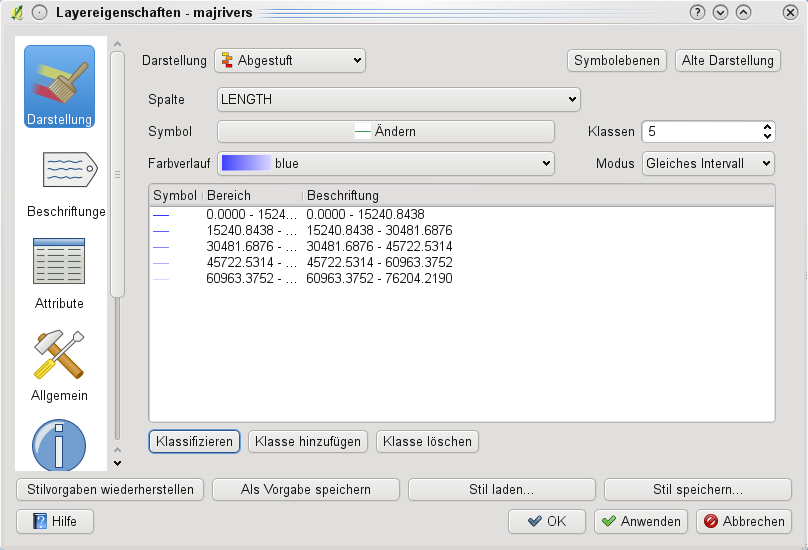
\includegraphics[clip=true, width=10cm]{graduatesymbol_ng_line}
   \caption{Opzioni di visualizzazione per Simbolo Graduato \wincaption}\label{fig:gradsymNG}
\end{figure}

\minisec{Visualizzatore Tramite regole}

Il visualizzatore Tramite regole rappresenta tutti gli elementi di un layer 
tramite simboli basati su regole, con i colori che riflettono la classificazione 
di un attributo di interesse. Le regole si basano su istruzioni SQL, che possono 
essere create con il Query Builder. È possibile creare raggruppamenti per regole 
in base ad un filtro o in funzione della scala ed è possibile definire il comportamento 
con 'Enable symbol levels' oppure con 'Use only first matched'.

L'esempio in figura \ref{fig:rulesymNG} mostra la finestra di dialogo per la visualizzazione 
tramite regole del layer rivers dei dati campione di \qg.

\begin{figure}[ht]
   \centering
   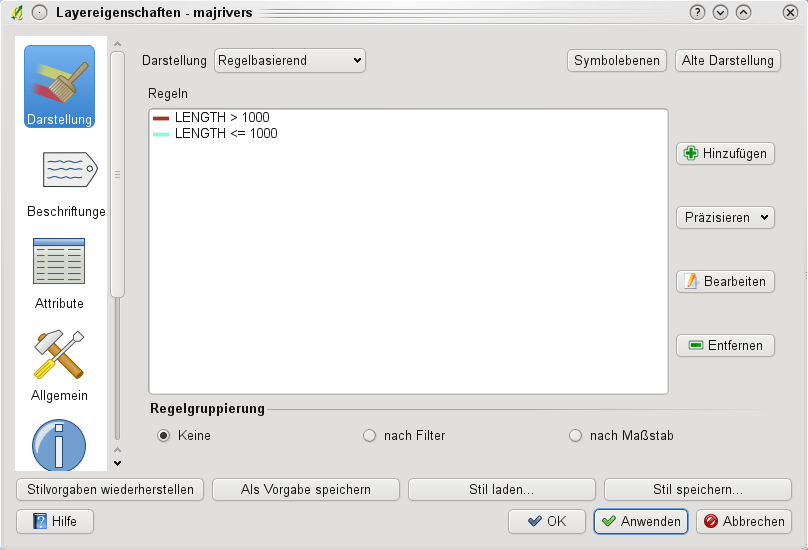
\includegraphics[clip=true, width=10cm]{rulesymbol_ng_line}
   \caption{Opzioni di visualizzazione per Simbolo Tramite regole \wincaption}\label{fig:rulesymNG}
\end{figure}

\minisec{Visualizzatore Spostamento punto}

Il visualizzatore Spostamento punto è attivo solo se si è caricato il Plugin Spostamento. 
Permette di visualizzare gli elementi di un layer di punti anche se hanno la stessa posizione.
I simboli vengono posizionati lungo un cerchio di spostamento intorno al centro del simbolo. 

\begin{figure}[ht]
   \centering
   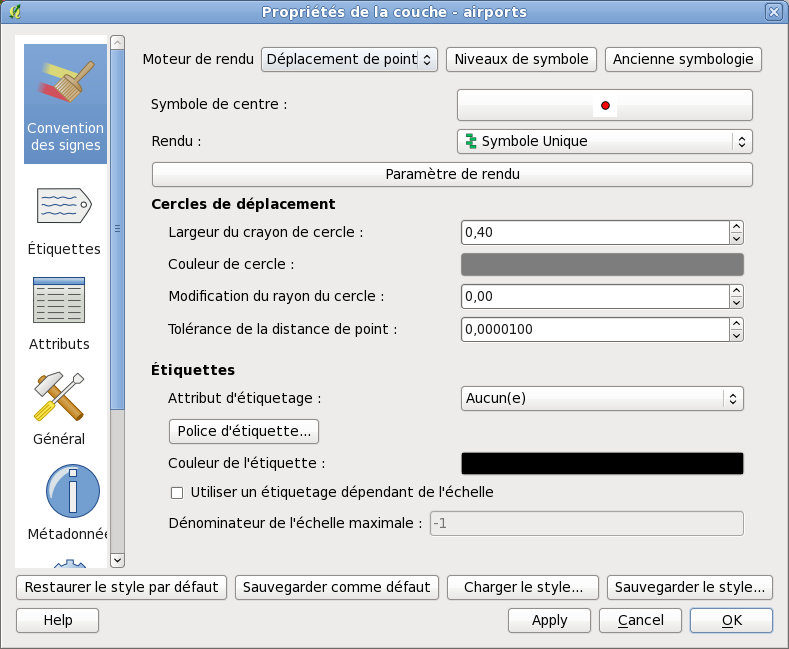
\includegraphics[clip=true, width=10cm]{poi_displacement}
   \caption{Finestra di dialogo del visualizzatore Spostamento punto \wincaption}\label{fig:poidissymNG}
\end{figure}

\minisec{Proprietà simbolo}

La finestra di dialogo Proprietà simbolo permette di impostare varie proprietà di un simbolo. 
Nella parte in basso a sinistra della finestra è disponibile un'anteprima del simbolo, così come 
apparirà nella vista mappa; sopra l'anteprima c'è la lista dei Layer simbolo. Per accedere alla 
finestra di dialogo Proprietà simbolo, cliccare su \dropmenuopttwo{mActionOptions}{Cambia} 
nella scheda \tab{Stile} della finestra di dialogo \dialog{Proprietà layer}.

È possibile aggiungere e rimuovere layer simbolo, cambiare al posizione dei layer oppure 
bloccare i layer ai cambiamenti di colore. Nella parte destra della finestra di dialogo è
possibile gestire le impostazioni di un layer simbolo selezionato nella lista Layer simbolo. 
L'impostazione più importante è 'Tipo layer del simbolo': le opzioni dipendono dal tipo 
di vettore (Punti, Linee, Poligoni).
  
\begin{description}
\item Opzioni Tipo layer del simbolo per vettori di punti
\begin{itemize}[label=--]
\item \textbf{Indicatore semplice}: Colore del bordo, Colore di riempimento, Dimensione, Angolo, Offset X,Y
\item \textbf{Indicatore SVG}: Dimensione, Angolo, Offset X,Y, Immagine SVG
\end{itemize}
\item Opzioni Tipo layer del simbolo per vettori di linee
\begin{itemize}[label=--]
\item \textbf{Decorazione linea}: Colore, Larghezze tratto
\item \textbf{Linea di evidenziazione}: Indicatore, Posizione indicatore, Indicatore di rotazione, Offset linea
\item \textbf{Linea semplice}: Colore, Larghezze del tratto, Offset, Stile tratto, Stile unione, Stile testa
\end{itemize}
\item Opzioni Tipo layer del simbolo per vettori di poligoni
\begin{itemize}[label=--]
\item \textbf{Riempimento con centroide}: Indicatore
\item \textbf{Riempimento SVG}: Larghezza della texture, Rotazione, Cornice
\item \textbf{Riempimento semplice}: Colore, Stile riempimento, Colore del bordo, Stile del bordo, Larghezza bordo, Offset
\item \textbf{Cornice: Decorazione semplice}: Colore, Larghezza tratto
\item \textbf{Cornice: Decorazione semplice}: Indicatore, Posizione indicatore, Indicatore di rotazione, Offset linea
\item \textbf{Cornice: linea semplice}: Colore, Larghezza tratto, Offset, Stile tratto, Stile unione, Stile testa
\end{itemize}
\end{description}

\begin{figure}[ht]
\centering
   \subfloat[Linea composta da tre linee semplici] {\label{subfig:symprops1}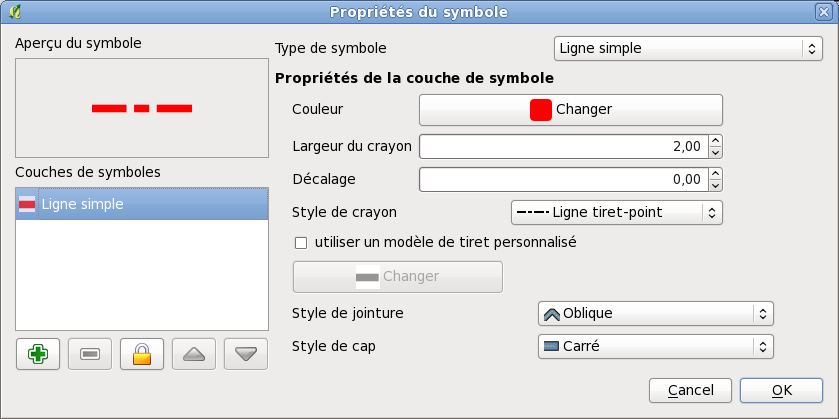
\includegraphics[clip=true, width=0.3\textwidth]{symbolproperties1}}
   \hspace{1cm}
   \subfloat[Proprietà simbolo per un layer di punti] {\label{subfig:symprops2}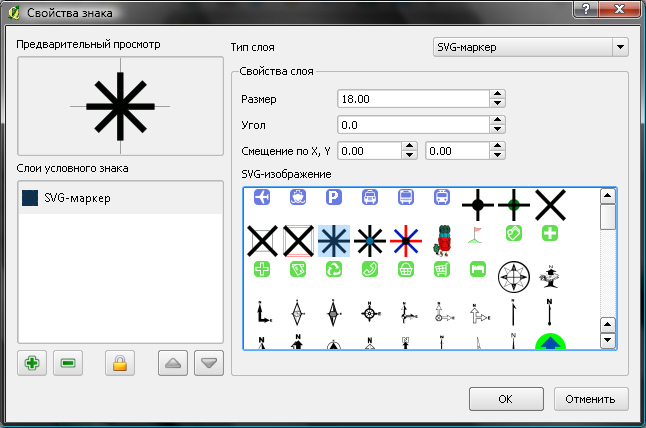
\includegraphics[clip=true, width=0.3\textwidth]{symbolproperties2}}
   \hspace{1cm}
   \subfloat[Schemi di riempimento per poligoni] {\label{subfig:symprops3}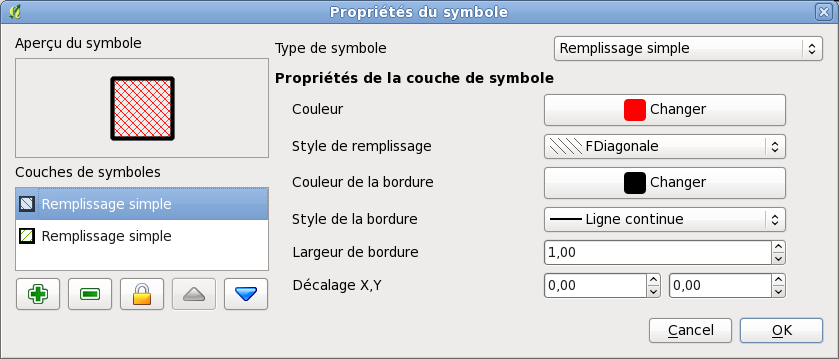
\includegraphics[clip=true, width=0.3\textwidth]{symbolproperties3}}
\caption{Definizione proprietà dei simboli \nixcaption}
\end{figure}

\subsection{Gestore stile}\label{subsec:stylemanager}

Il Gestore stile è una piccola applicazione di supporto alla gestione degli stili e delle 
loro componenti (simboli e scale di colori). Il gestore elenca i simboli e le scale di colori 
di uno stile e permette di modificarli, rimuoverli o aggiungerne di nuovi.
Per aprire il Gestore stile cliccare su \mainmenuopt{Impostazioni} \arrow 
\dropmenuopt{Gestore di stili...} nel menu principale.

\begin{figure}[ht]
   \centering
   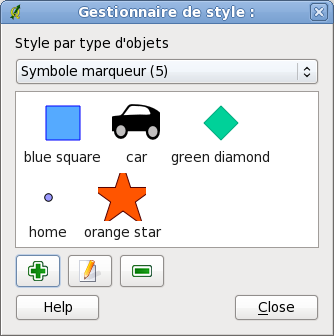
\includegraphics[clip=true, width=7cm]{stylemanager}
   \caption{Gestore stile \wincaption}\label{fig:stylemanager}
\end{figure}

\subsection{Vecchia simbologia}\label{sec:oldsymbology}
\index{layer vettoriali!vecchia simbologia}

\textbf{Nota}: \qg 1.7 supporta ancora la vecchia simbologia, sebbene sia raccomandato 
l'uso della simbologia di nuova generazione descritta in \ref{sec:symbology}; 
la vecchia simbologia sarà rimossa a partire dal prossimo rilascio di \qg.

Per utilizzare la vecchia simbologia cliccare su \button{Vecchia simbologia} nella 
scheda \tab{Stile} della finestra di dialogo \dialog{Proprietà layer}. 

È possibile usare la vecchia simbologia in modalità predefinita disattivando \checkbox{Utilizza la nuova 
generazione di simboli per la visualizzazione} nella scheda \tab{Visualizzazione} in
\mainmenuopt{Impostazioni} \arrow \dropmenuopt{Opzioni}.

La vecchia simbologia di \qg mette a disposizione i seguenti visualizzatori:

\begin{description} 
    \item[Simbolo singolo] - lo stesso stile è applicato a tutti gli elementi del vettore\index{layer vettoriali!stili!simbolo singolo}
    \item[Simbolo graduato] - lo stile applicato ai diversi elementi dipende
    dal valore di un campo particolare della tabella associata.\index{layer vettoriali!stili!simbolo graduato}
    \item[Colore continuo] - gli elementi del layer sono mostrati con una
    gradazione di colori compresa entro due estremi specificati in base ai valori numerici di uno specifico campo.\index{layer vettoriali!stili!colore continuo}
    \item[Valore univoco] - gli oggetti sono classificati in base ai valori
    unici di un campo della tabella associata, ad ogni valore viene assegnata una
    simbologia differente.\index{layer vettoriali!stili!valore unico}
\end{description}

Per modificare la simbologia di un layer, fare semplicemente doppio click
sulla relativa voce di legenda per fare apparire la finestra di dialogo
\dialog{Proprietà layer}.\index{simbologia!modifica}

\begin{figure}[ht]
\centering
\caption{Opzioni vecchia simbologia \nixcaption}
   \subfloat[Simbolo singolo] {\label{subfig:single_symbol}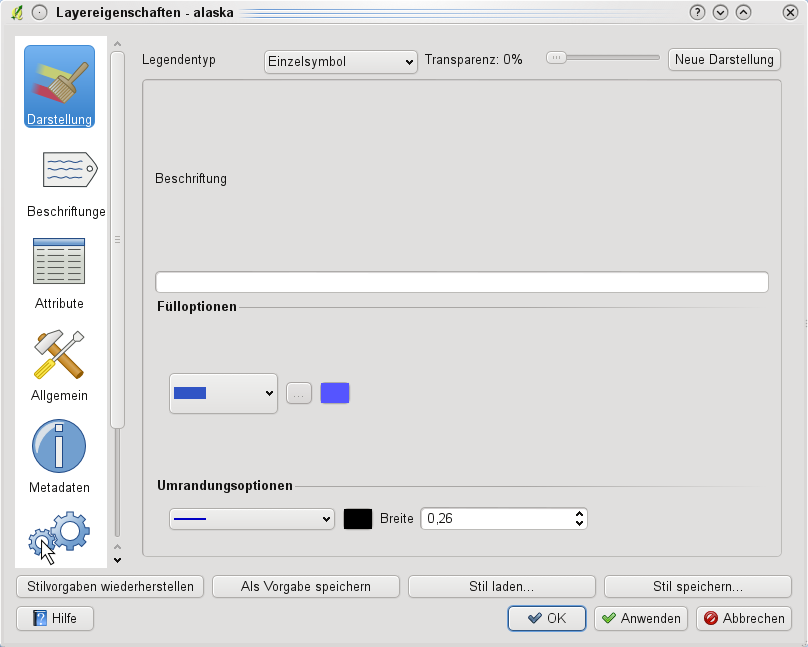
\includegraphics[clip=true, width=0.4\textwidth]{vectorClassifySingle}}
   \hspace{1cm}
   \subfloat[Simbolo graduato] {\label{subfig:graduated_symbol}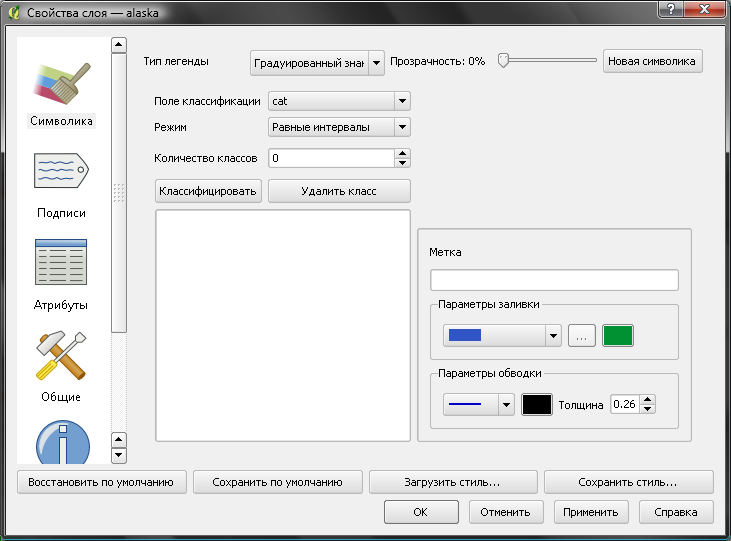
\includegraphics[clip=true, width=0.4\textwidth]{vectorClassifyGraduated}}
   \hspace{1cm}
   \subfloat[Colore continuo] {\label{subfig:cont_color}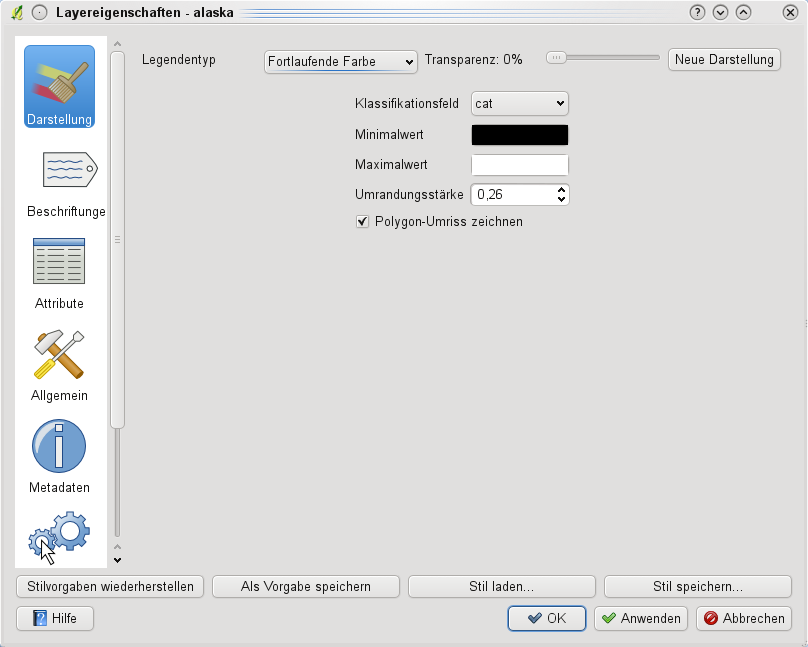
\includegraphics[clip=true, width=0.4\textwidth]{vectorClassifyContinous}}
   \hspace{1cm}
   \subfloat[Valore unico] {\label{subfig:unique_val}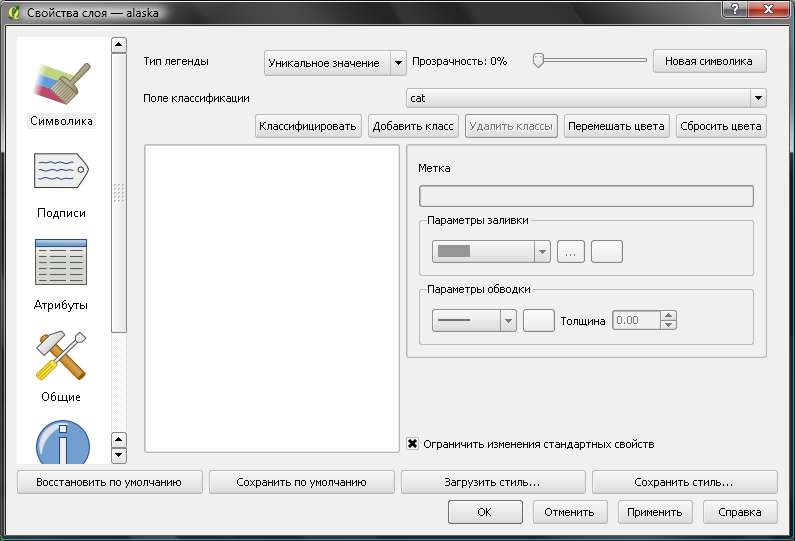
\includegraphics[clip=true, width=0.4\textwidth]{vectorClassifyUnique}}
\end{figure}

\minisec{Opzioni per lo stile} \label{sec:style_options} \index{layer vettoriali!stili}
In questa finestra di dialogo è possibile scegliere lo stile di
rappresentazione del layer vettoriale. Secondo l'opzione di visualizzazione
scelta tra quelle descritte precedentemente si ha la possibilità di
classificare anche gli elementi della mappa.

Le seguenti opzioni dovrebbero essere disponibili per pressoché tutte le
simbologie:

\begin{description}
\item[Opzioni riempimento]
\begin{description}
 \item[Stile riempimento] - stile per il riempimento. Oltre ai retini forniti è 
 possibile scegliere \selectstring{Stile di riempimento}{Texture} e cliccare su 
 \browsebutton per selezionare un retino personalizzato. Attualmente sono supportati 
 i formati: \filename{*.jpeg, *.xpm, and *.png}.
 \item[Colore di riempimento] - colore di riempimento degli elementi.
\end{description}
\item[Opzioni linea esterna]
\begin{description}
 \item[Stile bordo] - tipo di tratteggio del bordo degli elementi. Si può
 anche impostare l'opzione "Nessuno" per escludere la rappresentazione
 del contorno.
 \item[Colore bordo] - colore del bordo degli elementi
 \item[Spessore bordo] - larghezza della linea di contorno.
\end{description}
\end{description}

Lo stile di layer, una volta impostato, può essere salvato in un file (con 
estensione \filename{*.qml}): cliccare sul pulsante \button{Salva stile \ldots}. 
Il pulsante \button{Caricamento stile \ldots}, invece, carica un file di stile 
precedentemente salvato.

Se si desidera usare sempre un particolare stile quando il layer viene
caricato, cliccare su \button{Salva come predefinito} per rendere predefinito
lo stile impostato. Inoltre, se si effettuano modifiche delle quali
non si è soddisfatti, cliccare su \button{Ripristina stile predefinito} per
ritornare allo stile predefinito precedentemente impostato.

\minisec{Applicare la trasparenza ad un vettore} \label{sec:vect_transparency} \index{layer
vettoriali!trasparenza}
\qg permette di impostare la trasparenza per ogni layer vettoriale tramite la barra 
\slider{Trasparenza}{0}{20mm} nella scheda \tab{Stile} (Figura \ref{fig:vector_symbology}).
La trasparenza permette la visualizzazione di più layer vettoriali sovrapposti.

\subsection{Scheda Etichette}\label{labeltab}

Così come per la simbologia, anche per le etichette \qg 1.7 mette a disposizione
due modalità di gestione: di vecchia e di nuova generazione.
La scheda \tab{Etichette} ancora contiene l'etichettatura di vecchia generazione. 
L'etichettatura di nuova generazione è implementata con una nuova applicazione
che sostituirà la vecchia simbologia in una prossima versione di \qg.
Si raccomanda di utilizzare l'etichettatura di nuova generazione descritta nella 
Sezione \ref{newlabel}.

La scheda \tab{Etichette} consente di abilitare la visualizzazione delle
etichette associate agli elementi del layer e controlla una serie di
opzioni legate al posizionamento, allo stile e ad altre caratteristiche delle
etichette.

Come esempio visualizzeremo le etichette dello shapefile lakes del
\filename{\qg\_sample\_data}:

\begin{enumerate}
\item Caricare lo shapefile \filename{alaska.shp} e il file GML \filename{lakes.gml} in \qg.
\item Usare lo zoom su un'area a scelta contenente alcuni laghi.
\item Rendere attivo il layer \filename{lakes} cliccando su di esso nella
legenda.
\item Aprire la finestra di dialogo \dialog{Proprietà layer}.
\item Cliccare sulla scheda \tab{Etichette}.
\item Selezionare la casella di controllo \checkbox{Mostra etichette} per
abilitarne la visualizzazione.
\item Scegliere il campo della tabella contenente le etichette da visualizzare. 
  In questo esempio si userà \selectstring{Campo contenente etichetta}{NAMES}.
\item Inserire un'etichetta di default per gli elementi del layer lakes che
non hanno nome. Questa etichetta verrà quindi usata ogni volta che \qg dovrà
etichettare un lago al quale non corrisponde nessun valore nel campo \guilabel{NAMES}.
\item Nel caso di etichette molto lunghe, selezionare \checkbox{Etichette multilinea?}: 
\qg cercherà di posizionare l'etichetta opportunamente.
\item Cliccare su \button{Apply}.
\end{enumerate} 

Adesso sono visualizzate le etichette. Il loro aspetto non è probabilmente
gradevole, potrebbero essere troppo grandi e posizionate male in relazione al
simbolo dei laghi.

Cliccare allora su \button{Carattere} e \button{Colore}
per impostare il tipo di carattere e il colore. È possibile anche cambiare
l'angolo e la posizione delle etichette testuali.

Per modificare la posizione del testo rispetto agli elementi:

\begin{enumerate} 
\item Cliccare sulla scheda \tab{Etichette}.
\item Cambiare la posizione selezionando una delle opzioni disponibili nel
gruppo \classname{Posizionamento}. Nel caso preso in esame, scegliere l'opzione
\radiobuttonon{Destra}.
\item la voce \classname{Dimensioni carattere} consente di
selezionare tra \radiobuttonon{In punti} o \radiobuttonon{In unità mappa}.
\item Cliccare su \button{Apply} per visualizzare i cambiamenti senza chiudere
la finestra di dialogo.
\end{enumerate} 

Ora l'aspetto sarà migliore, ma le etichette appaiono ancora troppo vicine
all'indicatore della loro posizione. Per sistemare il problema è possibile
utilizzare l'opzione Offset: aggiungendo uno spostamento in X pari a 5
le etichette verranno scostate dall'indicatore della loro posizione e rese
più leggibili. Ovviamente più è grande l'indicatore o il carattere, maggiore
sarà lo scostamento da applicare.

Aggiungiamo infine un buffer sulle etichette cliccando sulla voce
\tab{Contorno etichette}. In questo modo verrà aggiunto uno sfondo attorno alle lettere
per farle risaltare maggiormente. Per mettere un buffer alle etichette dei
laghi procedere come di seguito:

\begin{enumerate}
\item Abilitare la casella di controllo \checkbox{Contorno etichette}.
\item Scegliere una dimensione (spessore) del buffer.
\item Scegliere un colore per il buffer cliccando sul pulsante
\button{Colore}. È inoltre possibile assegnare una trasparenza in percentuale
al buffer.
\item Cliccare su \button{Apply} per vedere i cambiamenti.
\end{enumerate} 

Modificare eventualmente i cambiamenti fino a quando non si è soddisfatti del
risultato, cliccando su \button{Apply} dopo ogni modifica.

In genere un buffer di 1 punto fornisce risultati esteticamente gradevoli.
Si noti che è anche possibile specificare la dimensione del buffer in unità
della mappa se ciò rende più agevole l'impostazione.

Le rimanenti voci della scheda \tab{Etichette} consentono di controllare
l'aspetto delle etichette usando, se adeguatamente preparati, gli attributi
del layer. Le voci della scheda \tab{Avanzato} consentono di settare
tutti i parametri delle etichette facendo riferimento a campi della tabella
del layer.

Si noti che la scheda \tab{Etichette} fornisce un'\classname{Anteprima}
nella quale viene mostrata l'etichetta predefinita.

\subsection{Nuova etichettatura}\index{Nuova etichettatura}\label{newlabel}

La nuova applicazione \toolbtntwo{labeling}{Etichettatura} richiede solo pochi 
parametri, ma gestisce in maniera intelligente l'etichettatura dei layer vettoriali; 
supporta, inoltre, i layer trasformati al volo.
Questa applicazione sostituirà l'etichettatura di vecchia generazione di \qg.

\minisec{Utilizzare la nuova etichettatura}

\begin{enumerate}
  \item Avviare QGIS e caricare un vettore.
  \item Attivare il layer nella legenda e cliccare sull'icona \toolbtntwo{labeling}{Etichettatura} 
  nel menu degli strumenti di QGIS.
\end{enumerate}

\minisec{Etichettare layer di punti}

Come prima cosa selezionare la casella di controllo \checkbox{Etichetta questo layer} e 
scegliere un campo della tabella degli attributi da usare per l'etichettatura. In seguito 
è possibile definire il posizionamento e lo stile del testo, la priorità, la visibilità in funzione 
della scala, se etichettare ogni parte delle geometrie multi-parte e se gli elementi 
devono comportarsi come ostacoli per le etichette (si veda Figura \ref{fig:pointlabel}).

\begin{figure}[ht]
\centering
   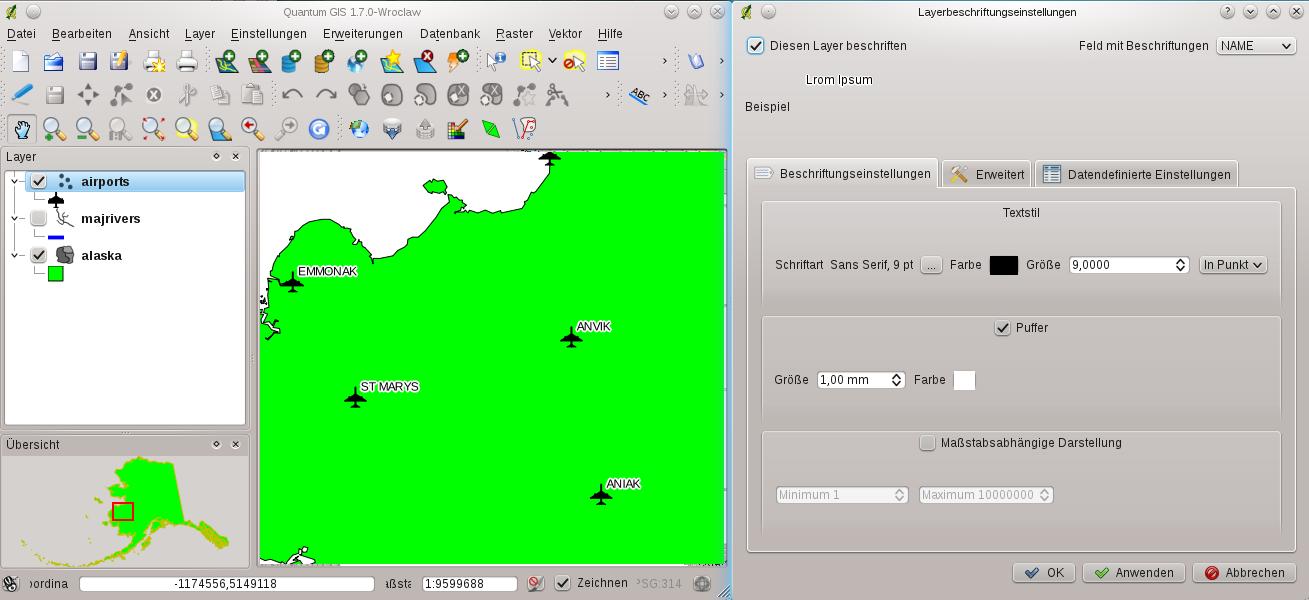
\includegraphics[clip=true, width=10cm]{label_points}
   \caption{Etichettatura intelligente di un layer di punti \nixcaption}\label{fig:pointlabel}
\end{figure}

\minisec{Etichettare layer di linee}

Come prima cosa selezionare la casella di controllo \checkbox{Etichetta questo layer} e 
scegliere un campo della tabella degli attributi da usare per l'etichettatura. In seguito 
è possibile definire il posizionamento dell'etichetta, l'orientamento, la distanza 
dagli elementi, lo stile del testo, la priorità, la visibilità in funzione della scala, 
se etichettare ogni parte delle geometrie multi-parte, se unire le linee collegate per evitare 
etichette doppie e se gli elementi devono comportarsi come ostacoli per le etichette 
(Figura \ref{fig:linelabel}).

\begin{figure}[ht]
\centering
   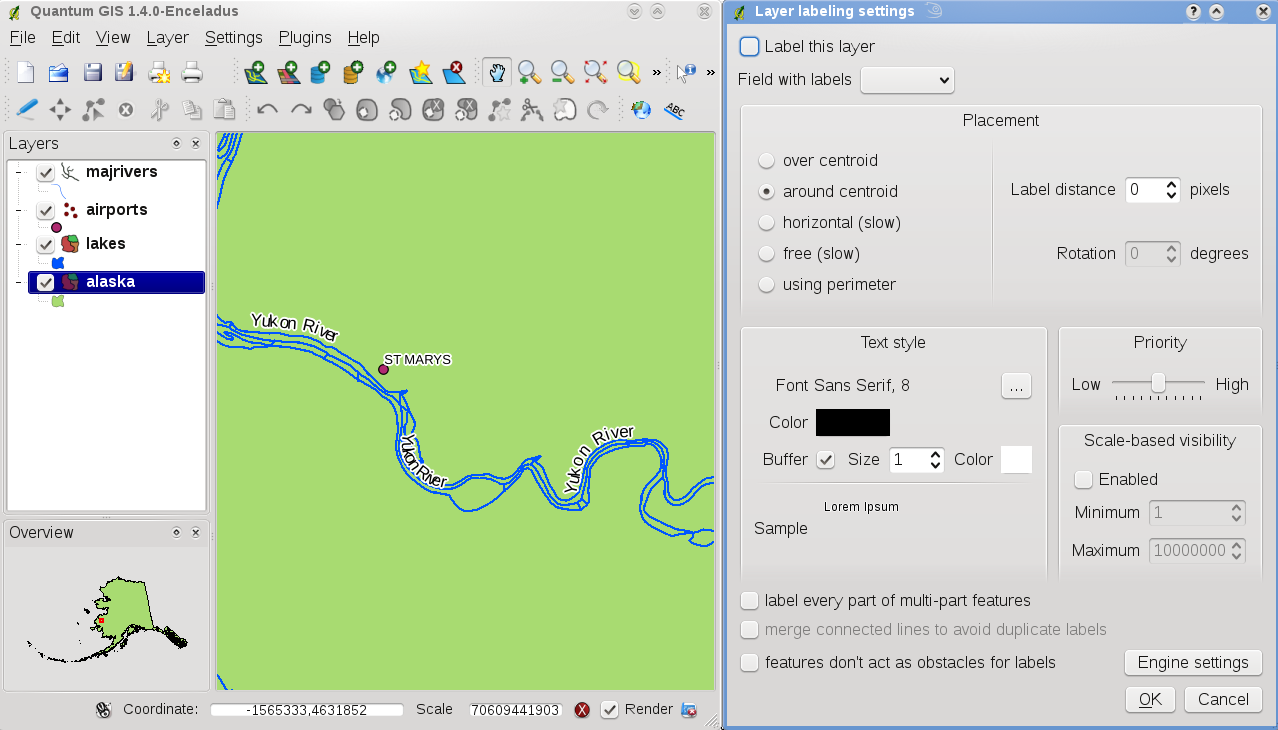
\includegraphics[clip=true, width=10cm]{label_line}
   \caption{Etichettatura intelligente di un layer di linee \nixcaption}\label{fig:linelabel}
\end{figure}

\minisec{Etichettare layer di poligoni}

Come prima cosa selezionare la casella di controllo \checkbox{Etichetta questo layer} e 
scegliere un campo della tabella degli attributi da usare per l'etichettatura. In seguito 
è possibile definire il posizionamento dell'etichetta, la distanza, lo stile del testo, la
priorità, la visibilità in funzione della scala, se etichettare ogni parte delle geometrie multi-parte,
e se gli elementi devono comportarsi come ostacoli per le etichette (Figura \ref{fig:arealabel}).

\begin{figure}[ht]
\centering
   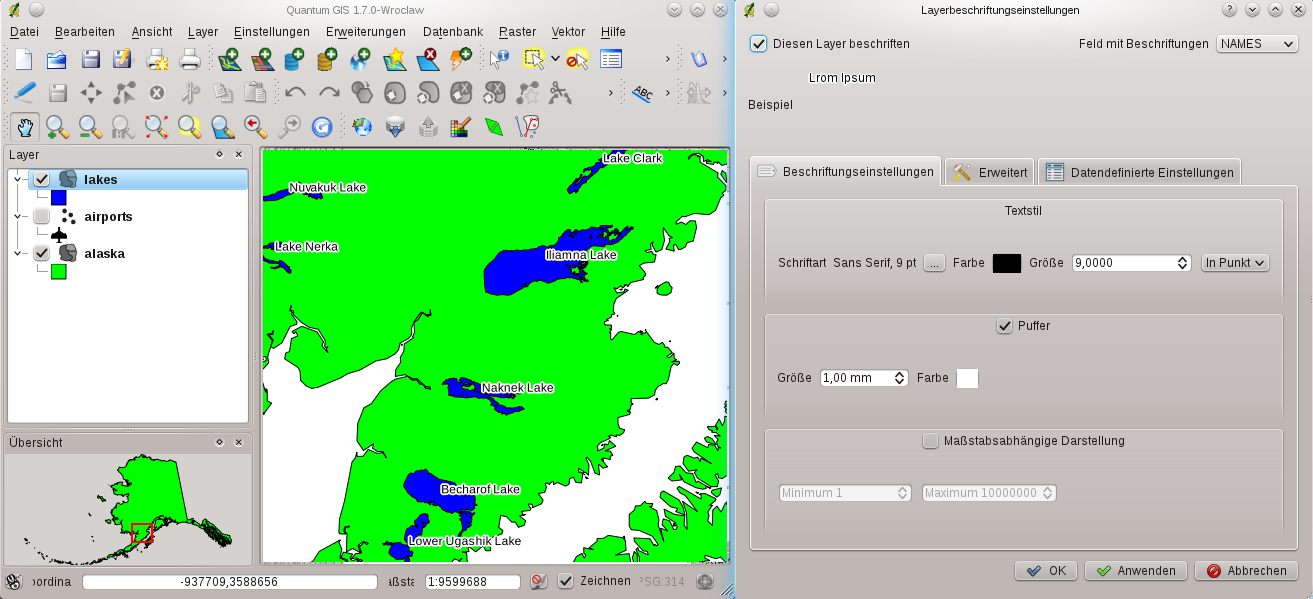
\includegraphics[clip=true, width=10cm]{label_area}
   \caption{Etichettatura intelligente di un layer di poligoni \nixcaption}\label{fig:arealabel}
\end{figure}

\minisec{Posizionamento etichette}

Cliccando sul pulsante \button{Impostazioni} nella scheda \tab{Avanzato} è possibile selezionare la modalità 
di ricerca per il posizionamento ottimale delle etichette. Le modalità disponibili sono: 
Catena, Popmusic tabu, Catena popmusic, Catena tabu popmusic e FALP.

\begin{figure}[ht]
\centering
   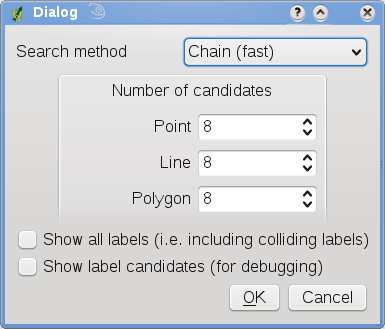
\includegraphics[clip=true, width=5cm]{label_engine}
   \caption{Finestra di dialogo delle modalità di ricerca \nixcaption}\label{fig:labelengine}
\end{figure}

Nella finestra di dialogo è possibile definire il numero di candidati, se mostrare tutte le 
etichette (incluse quelle che collidono) e se mostrare le etichette possibili (per debugging).

\minisec{Parole chiave in campi attributo per l'etichettatura}

È possibile usare alcune parole chiave in campi attributo dedicati per il posizionamento delle etichette:

\begin{itemize}[label=--]
\item \textbf{Per l'allineamento orizzontale}: left, center, right
\item \textbf{Per l'allineamento verticale}: bottom, base, half, top
\item \textbf{Colori specificati in motazione SVG}: e.g. \#ff0000
\item \textbf{Per bold, underlined, strikeout e italic}: 0 = false 1 = true
\end{itemize}

Combinazioni tipo 'base right' oppure 'bottom left' è possibile che funzionino.

\subsection{Scheda Campi}\index{Attributi}\label{label_attributes}

Con la scheda \tab{Campi} è possibile gestire gli attributi di un layer. I pulsanti 
\toolbtntwo{mActionNewAttribute}{Nuova colonna} \toolbtntwo{mActionDeleteAttribute}{Elimina colonna} 
possono essere usati se il layer è in \toolbtntwo{mActionToggleEditing}{Modalità di modifica}.

Allo stato attuale possono essere aggiunte/rimosse solo colonne di layer PostGIS. La libreria OGR 
supporta l'aggiunta di nuove colonne, ma non la rimozione, se si ha installata la versione 1.6 o 
superiore di GDAL.

Nel trac GDAL/OGR è presente un ticket con una patch in attesa di commit (\url{http://trac.osgeo.org/gdal/ticket/2671}). 
Nel frattempo, QGIS (ed ogni altro software che usa GDAL/OGR) ha una soluzione temporanea per cancellare 
colonne da uno Shapefile: tale soluzione è il plug-in di terze parti Table Manager.

\minisec{Widget modifica}

\begin{figure}[H]
   \begin{center}
   \caption{Finestra di dialogo per selezionare un widget di modifica di una colonna attributo \nixcaption}\label{fig:editwidget}\smallskip
   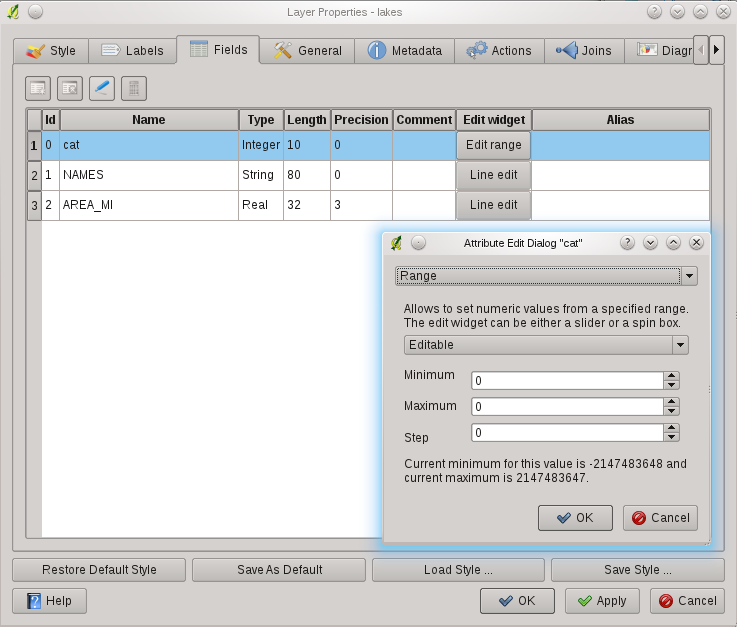
\includegraphics[clip=true, width=14cm]{editwidgetsdialog}
\end{center}
\end{figure}

Nella scheda \tab{Campi} è presente una colonna \texttt{Widget modifica}: questa può essere usata per definire 
valori o intervalli di valori permessi per gli attributi. Cliccando su \button{Modifica valore} si apre una finestra 
di dialogo dove è possibile definire diversi widget:

\begin{itemize}
\item Modifica valore: widget predefinito. Supporta testo semplice o numeri per attributi numerici.
\item Classificazione: visualizza una combo-box contenente i valori utilizzati per la classificazione, 
qualora il tipo di legenda (nella scheda stile) sia stato impostato su 'valore unico'.
\item Intervallo: permette di definire un numero di valori per un intervallo specifico. Il widget 
di modifica può utilizzare un cursore o una casella di selezione.
\item Valori unici: l'utente può selezionare uno dei valori già utilizzati negli attributi. Se editabile, 
una linea modificata ha la possibilità di autocompletamento; in caso contrario viene presentata una combo-box.
\item Nome file: semplifica la selezione di file attraverso una finestra di dialogo di scelta.
\item Mappa valori: combo-box con oggetti predefiniti. Il valore è archiviato negli attributi, la descrizione 
presentata nel combo-box. I valori possono essere definiti manualmente o caricati da un layer o da un file csv.
\item Enumerazione: apre una combo-box con i valori che possono essere utilizzati. È supportato solo dal 
provider postgres.
\item Immutabile: l'attributo è di sola lettura, non può essere modificato.
\item Nascosto: l'attributo è invisibile all'utente.
\item Checkbox.
\end{itemize}

\subsection{Scheda Generale}\label{vectorgeneraltab}

La scheda \tab{Generale} è sostanzialmente simile a quella dei raster. Essa 
consente di cambiare il nome del file mostrato, impostare la visualizzazione
in base alla scala, creare un indice spaziale (solo per i formati supportati
da OGR e per layer PostGIS) e vedere o cambiare la proiezione del layer.

Il pulsante \button{Query Builder} consente di selezionare un sottoinsieme
di elementi nel layer, ma attualmente questa query di selezione funziona solo 
se si apre la tabella degli attributi e si clicca su \button{Ricerca avanzata}.

\subsection{Scheda Metadati}\index{Metadati}

La scheda \tab{Metadati} contiene informazioni sul layer, come ad esempio il tipo, 
la localizzazione, il numero ed il tipo di elementi, le possibilità di modifica. 
La sezione \guiheading{Estensione} fornisce informazioni sull'estensione territoriale 
dei dati, mentre la sezione \guiheading{Sistema di Riferimento Spaziale del layer} fornisce 
informazioni sul SR. La scheda \tab{Metadati} non è attualmente editabile.

\subsection{Scheda Azioni}\index{Azioni}\label{label_actions}

\qg offre la possibilità di effettuare azioni sulla base degli
attributi associati ai singoli elementi del layer vettoriale.
Questo permette di effettuare un elevato numero di azioni, per esempio,
lanciare un programma con argomenti costruiti tramite gli attributi
delle geometrie o passando i parametri ad uno strumento di web reporting.

Definire delle azioni è utile quando si intende lanciare un'applicazione
esterna o la visualizzazione di una pagina web sulla base di uno o più valori
associati al layer vettoriale. Ad esempio si può lanciare una ricerca web
basata sul valore di un attributo. Questo concetto è spiegato nel seguente
paragrafo.

\minisec{Definire le azioni}\index{azioni!definizione}

Le azioni legate agli attributi sono definite dalla finestra di dialogo
\dialog{Proprietà layer}. Per impostare un'azione, aprire la finestra
di dialogo \dialog{Proprietà layer} e cliccare sulla scheda \tab{Azioni}. 
Fornire una descrizione per l'azione nel campo Nome. L'azione in
sé deve contenere il nome o il percorso di una applicazione che verrà eseguita quando
l'azione viene richiamata. L'azione può venire fatta dipendere da uno o più campi della tabella
attributi. Quando essa è richiamata ogni stringa testuale che inizia con \%
seguita dal nome di un campo della tabella attributi verrà rimpiazzata dal
valore di quel campo. I caratteri speciali \%\% \index{caratteri speciali \%\%}saranno
rimpiazzati dal valore del campo nell'elemento selezionato con lo strumento
"Informazioni elementi" disponibile nella barra strumenti o dalla tabella attributi (si veda il paragrafo seguente 'Usare le azioni). 
Le virgolette (") possono essere usate per raggruppare il testo in un singolo argomento da
passare al programma, allo script o al comando che si intende eseguire Le
virgolette saranno ignorate se precedute dalla barra inversa.

Se sono presenti nomi di campi che possono essere interpretati come
sotto-stringhe di altri nomi di campi (ad es. \usertext{col1} e
\usertext{col10}) è necessario racchiudere il nome (e il
carattere \%) tra parentesi quadre (ad es. \usertext{[\%col10]}). Ciò impedirà
che il nome di campo \usertext{\%col10} possa essere confuso con
\usertext{\%col1} con uno \usertext{0} alla fine. Le virgolette saranno
rimosse da \qg man mano che vengono inseriti i valori del campo al posto
dell'espressione. Se si vuole che i campi sostituiti vengano racchiusi entro
parentesi quadre, aggiungere una seconda coppia di parentesi quadre in questo
modo: \usertext{[[\%col10]]}.

La finestra di dialogo \dialog{Informazioni sui risultati} che compare quando si
usa lo strumento "Informazioni elementi" ha una voce {\em (Derivato)} che
contiene informazioni dipendenti dal tipo di layer interrogato. Si
può accedere ai valori di questa voce similmente a come si accede ai valori
di campo della tabella attributi anteponendo al nome di campo disponibile alla
voce {\em (Derivato)} l'espressione \usertext{(Derivato).}. Per esempio un
layer puntuale ha due sotto-voci \usertext{X} e \usertext{Y} e il valore di
essi può essere usato nell'azione con l'espressione \usertext{\%(Derivato).X}
e \usertext{\%(Derivato).Y}. Gli attributi derivati sono disponibili solo nella
finestra \dialog{Informazioni sui risultati} aperta dallo strumento 
\toolbtntwo{mActionOpenTable}{Informazioni elementi} e non nella finestra 
\dialog{Tabella degli attributi}.

Due esempi di azioni sono di seguito indicati:\index{azioni!esempi}

\begin{itemize}
  \item \usertext{konqueror http://www.google.com/search?q=\%nam}
  \item \usertext{konqueror http://www.google.com/search?q=\%\%}
\end{itemize}

Nel primo esempio, il browser konqueror viene richiamato con un URL da
aprire. L'URL crea una ricerca Google sul valore del campo \usertext{nam} nel
layer vettoriale. Si noti che il programma o lo script richiamato dall'azione
deve essere nel path impostato come variabile d'ambiente oppure bisogna
fornire il percorso completo all'eseguibile. Per sicurezza, è possibile
riscrivere il primo esempio come: \usertext{/opt/kde3/bin/konqueror
http://www.google.com/search?q=\%nam}. In questo modo si è sicuri che
l'applicazione konqueror sarà eseguita quando si richiama l'azione.

Nel secondo esempio viene usata la notazione \%\% che non richiede
l'indicazione di un particolare campo. Quando si richiama l'azione, il \%\%
sarà rimpiazzato dal valore selezionato con lo strumento \toolbtntwo{mActionOpenTable}{Informazioni elementi} 
o nella tabella attributi.

\minisec{Uso delle azioni}\index{azioni!uso}\label{label_usingactions}

Le azioni posso essere richiamate sia dalla finestra \dialog{Informazioni sui risultati} 
che da quella della \dialog{Tabella degli attributi}. 
(Si ricorda che queste finestre possono essere aperte rispettivamente cliccando sullo
strumento \toolbtntwo{mActionOpenTable}{Informazioni elementi} o
\toolbtntwo{mActionOpenTable}{Apri tabella attributi}.)
Per eseguire l'azione, fare click con il tasto destro del mouse sul record e scegliere
azione dal menu contestuale. Le azioni sono indicate nel menu a contestuale dal
nome assegnatogli in fase di definizione dell'azione. Cliccare sull'azione che
si vuole eseguire.

Se si vuole eseguire un'azione che usa la notazione \%\%, cliccare con il tasto destro del mouse
sul valore di campo che si desidera passare all'azione nella finestra di dialogo \dialog{Informazioni sui risultati} 
o in quella \dialog{Tabella degli attributi}.

In questo altro esempio viene illustrato come estrarre dati da un layer
vettoriale per inserirli in un file usando la shell di sistema bash e il
comando \usertext{echo} (dunque funzionerà solo su \nix e forse su \osx). Il
layer in questione ha i seguenti campi nella tabella attributi: nome della
specie \usertext{taxon\_name}, latitudine \usertext{lat} e longitudine
\usertext{long}. Si vuole eseguire una selezione spaziale delle specie
(taxon) presenti in determinate posizioni esportando i risultati in un file di
testo per le posizioni selezionate (evidenziate in giallo nella
vista mappa di \qg). L'azione in grado di assolvere lo scopo è la seguente:

\begin{verbatim}
  bash -c "echo \"%taxon_name %lat %long\" >> /tmp/species_localities.txt"
\end{verbatim} 

Selezionando alcune posizioni, l'esecuzione dell'azione precedente su ognuna
di esse genera un file in uscita che avrà l'aspetto seguente:

\begin{verbatim}
  Acacia mearnsii -34.0800000000 150.0800000000
  Acacia mearnsii -34.9000000000 150.1200000000
  Acacia mearnsii -35.2200000000 149.9300000000
  Acacia mearnsii -32.2700000000 150.4100000000
\end{verbatim} 

Come esercizio si può creare un'azione che generi una ricerca su Google sul
layer \filename{lakes}. Innanzitutto è necessario determinare la sintassi da
impiegare nell'URL per eseguire una ricerca basata su una parola chiave.
L'espressione si ricava facilmente eseguendo una ricerca dalla pagina di
Google, la pagina dei risultati avrà un indirizzo, visibile nella barra
indirizzi del browser, del tipo: \url{http://google.com/search?q=qgis},
in cui \usertext{qgis} è la parola ricercata. Forniti di questa informazione,
si può procedere nel seguente modo:

\begin{enumerate}
\item Assicurarsi che il layer \filename{lakes} sia caricato.
\item Aprire la finestra di dialogo \dialog{Proprietà layer} facendo
doppio click sul layer o cliccando su di esso nella legenda con il tasto
destro del mouse e scegliendo \dropmenuopt{Proprietà} dal menu contestuale.
\item Cliccare sulla scheda \tab{Azioni}.
\item Inserire un nome descrittivo per l'azione, ad esempio \usertext{Google}.
\item Fornire il nome di un programma esterno da eseguire nell'azione. In
questo caso useremo il browser Firefox. Se il programma non si trova in uno
dei percorsi di sistema definiti dalla variabile d'ambiente PATH, bisogna
specificare il percorso completo all'eseguibile.
\item Far seguire il nome del programma esterno dall'URL usato per la ricerca
su Google senza includere la parola ricercata, ovvero:
  \url{http://google.com/search?q=}
\item A questo punto il testo nel campo \guilabel{Azioni} dovrebbe apparire
così:\\
  \usertext{firefox \url{http://google.com/search?q=}}
\item Cliccare sul menu a tendina contenente i nomi dei campi della tabella
associata al layer \usertext{lakes}, posizionato immediatamente a sinistra del
pulsante \button{Inserisci campo}.
\item Dall'elenco apparso scegliere \selectstring{}{NAMES} e cliccare su \button{Inserisci campo}.
\item Il testo dell'azione dovrebbe ora apparire come segue:\\ \usertext{firefox
  \url{http://google.com/search?q=\%NAMES}}
\item Per completare l'azione cliccare sul pulsante \button{Inserisci l'azione}.
\end{enumerate}
 
Questo completa la definizione dell'azione che è così pronta per essere usata.
La formulazione finale dell'azione dovrebbe apparire così:

\begin{center}
\usertext{firefox \url{http://google.com/search?q=\%NAMES}}
\end{center}

A questo punto l'azione è pronta per essere usata. Chiudere la finestra
\dialog{Proprietà layer} e usare lo zoom su un'area a scelta. Assicurarsi
che il layer \filename{lakes} sia attivo ed identificare con l'apposito
strumento un lago. Nella finestra risultante dovrebbe essere visibile l'azione:

\begin{figure}[ht]
   \begin{center}
   \caption{Selezione di un elemento e scelta dell'azione \nixcaption}\label{fig:identify_action}\smallskip
   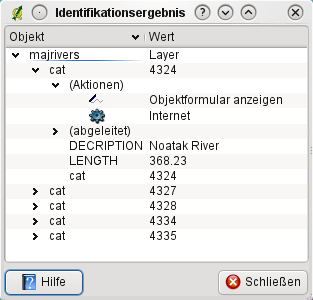
\includegraphics[clip=true, width=8cm]{action_identifyaction} 
\end{center}  
\end{figure}

Cliccando sull'azione, viene lanciato Firefox all'URL
\url{http://www.google.com/search?q=Tustumena}. È anche possibile aggiungere
ulteriori campi all'azione, inserendo un '+' alla fine della stringa che
definisce l'azione, selezionando quindi un altro campo e cliccando sul
pulsante \button{Inserisci campo}. Nell'esempio seguito finora semplicemente non c'è alcun
altro campo sul quale avrebbe senso fare una ricerca.

È possibile definire più di un'azione per ogni layer, ognuna di esse verrà
mostrata nella finestra \dialog{Informazioni sui risultati}. Si possono anche
eseguire azioni dalla tabella attributi cliccando con il tasto destro su una
riga selezionata e scegliendo dal menu contestuale l'azione desiderata.

Si possono immaginare molti tipi di azione. Ad esempio se un layer di punti
rappresenta le posizioni alle quali sono state scattate foto o alle quali
corrispondono immagini e il nome dei file di tali foto o immagini, è possibile
creare un'azione per lanciare un visualizzatore che mostri l'immagine. Le
azioni possono essere usate anche per lanciare report sul web per uno o più
campi della tabella attributo, definendole allo stesso modo dell'esempio per la ricerca con Google.

\subsection{Scheda Join}\label{sec:joins}
\index{layer vettoriali!join}

La scheda \tab{Join} permette di effettuare un join tra una tabella di attributi ed 
un layer vettoriale, indicando il layer da unire, il campo unione ed il campo di destinazione.
Attualmente QGIS permette il join di tabelle nei formati supportati da OGR, testo delimitato 
e del provider PostgreSQL (Figura~\ref{fig:join_attributes}).

\begin{figure}[ht]
   \centering
   
\includegraphics[clip=true, width=8cm]{join_attributes}
   \caption{Join di una tabella di attributi e di un layer vettoriale \nixcaption}
   \label{fig:join_attributes}
\end{figure}

Il dialogo del join vettoriale fornisce le opzioni:

\begin{itemize}[label=--]
\item \checkbox{Layer unito in memoria virtuale}
\item \checkbox{Crea un indice nel campo unito}
\end{itemize}

\subsection{Scheda Diagrammi}\label{sec:diagram}
\index{layer vettoriali!diagrammi}

La scheda \tab{Diagrammi} permette di sovrapporre un grafico ad un layer vettoriale (Figura~\ref{fig:diagramtab}).

\begin{figure}[ht]
   \centering
   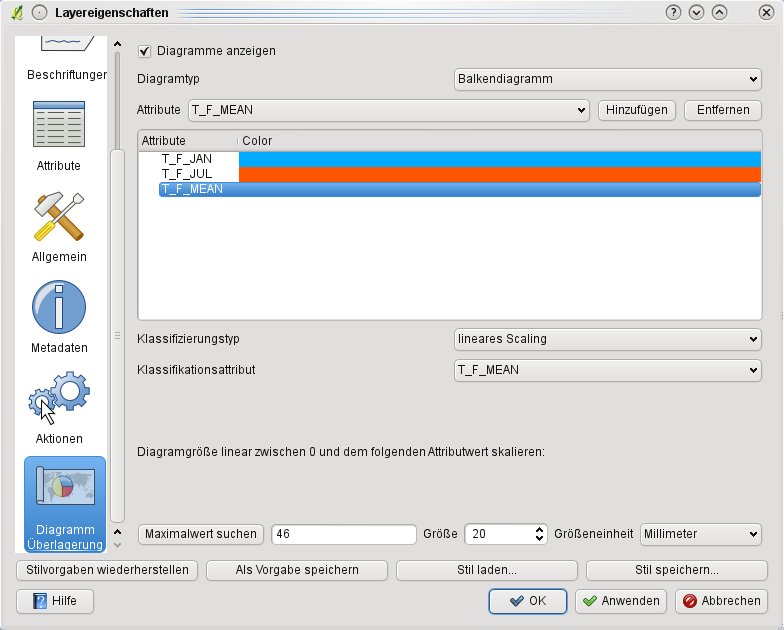
\includegraphics[clip=true, width=13cm]{diagram_tab}
   \caption{Scheda diagrammi \nixcaption}
   \label{fig:diagramtab}
\end{figure}

L'implementazione corrente dei diagrammi supporta grafici a torta e diagrammi testo e 
permette di scalare linearmente il grafico in funzione di un attributo.
Il posizionamento del grafico interagisce con l'etichettatura di nuova generazione. 
Segue un esempio di creazione di un grafico delle temperature
sovrapposto al layer alaska; entrambi i layer sono disponibili nei dati campione di \qg 
(Sezione~\ref{label_sampledata}).

\begin{enumerate}
\item Cliccare sull'icona \toolbtntwo{mActionAddOgrLayer}{Aggiungi vettore} e 
caricare i due vettori \filename{alaska.shp} e \filename{climate.shp}.
\item Doppio click sul layer \filename{climate} nella legenda per aprire la finestra di dialogo 
\dialog{Proprietà layer}.
\item Selezionare \button{Grafico a torta} nella scheda \tab{Diagrammi}.
\item Il grafico dovrà mostrare i valori dei campi:
\filename{T\_F\_JAN, T\_F\_JUL} e \filename{T\_F\_MEAN}. Selezionare
\filename{T\_F\_JAN} in Attributi e cliccare il pulsante verde \button{+}, quindi
\filename{T\_F\_JUL} ed alla fine \filename{T\_F\_MEAN}.
\item Scalare linearmente in funzione dell'attributo \filename{T\_F\_JUL}.
\item Cliccare su \button{Trova valore massimo}, scegliere 10 come dimensione e cliccare 
su \button{Apply} per visualizzare il grafico nella finestra principale di \qg.
\item Modificare (dimensioni, colori, etc.) in funzione delle esigenze.
\item Cliccare su \button{Ok} per completare l'operazione.

Il risultato è visibile in Figura~\ref{fig:climatediagram}.

\end{enumerate}

\begin{figure}[ht]
   \centering
   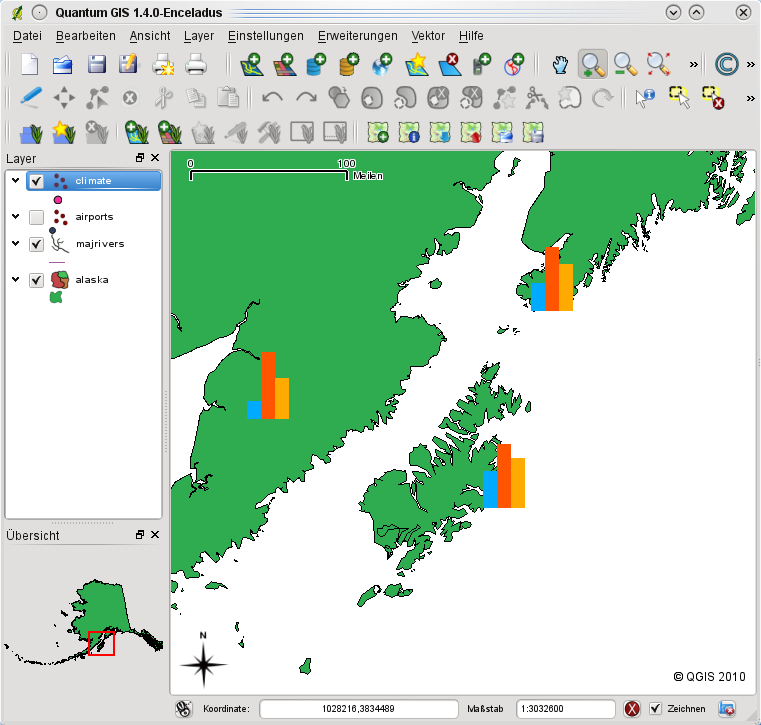
\includegraphics[clip=true, width=13cm]{climate_diagram}
   \caption{Grafico delle temperature sovrapposto ad una mappa \nixcaption}
   \label{fig:climatediagram}
\end{figure}

\section{Modifica}\index{modifica}

\qg supporta la modifica di layer vettoriali OGR, PostGIS e Spatialite. 
\textbf{Nota} - la modifica di layer GRASS segue una procedura diversa - 
si veda Sezione \ref{grass_digitising} per maggiori dettagli. 

\begin{Tip}\caption{\textsc{Modifiche concorrenti}}
Questa versione di QGIS non effettua alcuna verifica sulla possibilità che più 
utenti stiano effettuando contemporaneamente modifiche sullo stesso layer, è quindi 
l'ultimo utente che effettua il salvataggio ad apportare le modifiche definitive.
\end{Tip}

\subsection{Settare la tolleranza dello snapping e il raggio di ricerca degli elementi}\label{sec:snapping_tolerance}
\index{tolleranza di snapping}

Prima di editare vertici, è molto importante sia impostare il livello di snapping
che il valore del raggio di ricerca al fine di gestire in maniera ottimale la modifica delle
geometrie di un layer vettoriale. 

\minisec{Tolleranza di snapping}

La tolleranza di snapping è la distanza entro la quale \qg
\usertext{cerca} il vertice e/o segmento più vicino al quale si cerca di
agganciarsi quando si crea un nuovo vertice o si sposta un vertice esistente.
Se non si è entro la tolleranza di snapping, QGIS lascerà il vertice creato o
spostato nella posizione in cui si rilascia il pulsante del mouse invece di
agganciarlo ad un vertice e/o segmento esistente. 
La tolleranza di snapping influenza tutti gli strumenti che lavorano con una tolleranza.

\begin{enumerate}
\item La tolleranza di snapping può essere impostata a livello dell'intero 
progetto scegliendo la voce di menu \mainmenuopt{Impostazioni} \arrow \dropmenuopttwo{mActionOptions}{Opzioni}.
Nella scheda \tab{Digitalizzazione} è possibile impostare la modalità di
snap predefinita tra snap al vertice, al segmento o entrambe. Si può anche
definire una tolleranza di snapping e un raggio di ricerca per la modifica di
un vertice, in unità di mappa o in pixel. Impostando i valori in pixel, invece 
che in unità di mappa, si evita di dover modificare la tolleranza in seguito 
ad operazioni di zoom. 

\item È anche possibile impostare una tolleranza di snapping per 
singolo layer scegliendo la voce di menu \mainmenuopt{Impostazioni} \arrow
\button{Opzioni di snap\dots} (Figura~\ref{fig:snappingoptions}).
\end{enumerate}

\begin{figure}[H]
   \begin{center}
   \caption{Modifica delle opzioni di snapping per singoli layer \wincaption}\label{fig:snappingoptions}\smallskip
   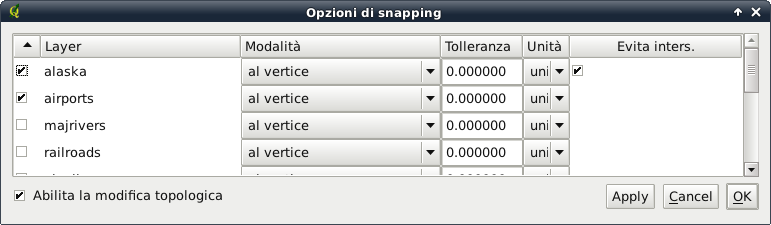
\includegraphics[clip=true, width=14cm]{editProjectSnapping} 
\end{center}  
\end{figure}

\minisec{Raggio di ricerca}

Il raggio di ricerca è la distanza che QGIS usa per \usertext{cercare} il 
vertice più vicino che si sta provando a spostare quando si clicca nella mappa.
Se non si è entro il raggio di ricerca, QGIS non troverà né selezionerà alcun vertice 
e mostrerà un avvertimento in una finestra pop-up.
La tolleranza di snapping e il raggio di ricerca sono impostati in unità di
mappa o in pixel e potrebbe essere necessario fare diversi tentativi prima di trovare
l'impostazione migliore. Se si specifica una tolleranza troppo alta, QGIS
potrebbe agganciare il vertice sbagliato, specialmente se si ha a che fare con
molti vertici vicini all'area in cui si sta effettuando la modifica.
Impostando invece un raggio di ricerca troppo piccolo impedirà a QGIS
di trovare alcuna geometria da spostare.

Il raggio di ricerca per la modifica di vertici può essere definito in unità
del layer dalla scheda \tab{Digitalizzazione} sotto il menu
\mainmenuopt{Impostazioni} \arrow \dropmenuopttwo{mActionOptions}{Opzioni}, sotto lo
stesso percorso dal quale è possibile impostare la tolleranza di snapping a
livello di progetto.

\subsection{Zoom e spostamento}

Prima di editare un layer sarebbe opportuno ingrandire la vista mappa su un'area 
di interesse, al fine di evitare una lunga attesa per la visualizzazione di tutti 
i vertici della mappa. 

Oltre ad utilizzare le icone \toolbtntwo{mActionPan}{Sposta mappa} e
\toolbtntwo{mActionZoomIn}{Ingrandisci}/\toolbtntwo{mActionZoomOut}{Rimpicciolisci}, 
è possibile interagire con la mappa con la rotellina del mouse, la barra spaziatrice
e i tasti freccia della tastiera.

\minisec{Zoom e spostamento con la rotella del mouse}

Per spostarsi nella mappa cliccare sulla rotella del mouse e trascinare, mentre 
per lo zoom basta ruotare la stessa. Posizionare il cursore nell'area di mappa e 
ruotare la rotellina verso di sé per ridurre e verso lo schermo per ingrandire. La
posizione del puntatore del mouse determinerà il centro dell'area da ingrandire. 
È possibile personalizzare il comportamento della rotella del mouse nella scheda 
\tab{Strumenti mappa} alla voce di menu \mainmenuopt{Impostazioni} \arrow \dropmenuopt{Opzioni}.

\minisec{Spostamento con i tasti freccia}

È possibile spostare la vista mappa anche con i tasti freccia della tastiera. 
Posizionare il mouse nella vista mappa e cliccare la freccia destra per spostarsi 
verso est, la freccia sinistra per spostarsi verso ovest, la freccia in su per 
spostarsi verso nord e la freccia in giù per spostarsi verso sud.

È anche possibile tenere premuta la barra spaziatrice mentre si sposta il
mouse per spostare la vista mappa e usare i tasti PgUp e PgDown per aumentare
o ridurre l'ingrandimento senza interrompere la sessione di digitalizzazione.

\subsection{Modifiche topologiche}

Oltre alle opzioni di snap a livello di singolo layer, la finestra di dialogo
\mainmenuopt{Impostazioni} \arrow \dropmenuopttwo{mActionOptions}{Opzioni di snap\dots} 
permette di impostare altre funzionalità topologiche. È possibile selezionare 
le opzioni \checkbox{Abilita la modifica topologica} e \checkbox{Evita inters.}:
quest'ultima evita l'intersezione di nuovi poligoni.

\minisec{Abilitare la modifica topologica}

L'opzione \checkbox{Abilita la modifica topologica} serve a mantenere bordi
comuni tra poligoni adiacenti durante l'editazione. QGIS "individua" un bordo
condiviso in un insieme di poligoni e tutto ciò che si deve fare è spostare il
vertice una volta sola: QGIS si occuperà di aggiornare i bordi di poligoni adiacenti.

\minisec{Evitare le intersezioni per i nuovi poligoni}

L'opzione \checkbox{Evita inters.} impedisce l'intersezione di poligoni adiacenti, 
rendendone più spedita la digitalizzazione. Se si ha già un poligono, è possibile con 
questa opzione abilitata digitalizzare un secondo poligono in modo che entrambi si 
intersechino; QGIS taglierà automaticamente il secondo lungo il bordo comune, con il vantaggio che
l'utente non deve digitalizzare tutti i vertici coincidenti.

\subsection{Modifica di un layer esistente}
\index{layer vettoriali!modifica}
\index{modifica!layer esistente}
\label{sec:edit_existing_layer}

Al fine di evitare modifiche involontarie, i dati sono caricati in QGIS 
in modalità solo lettura. Comunque, è sempre possibile modificare un layer 
se ciò è consentito dallo specifico fornitore di dati (es. se OGR supporta 
lo specifico formato in lettura/scrittura) e se il dato medesimo è anche 
scrivibile (ovvero i file non sono in modalità sola lettura).

Le funzioni di modifica di layer sono più versatili quando sono applicate a
dati immagazzinati in database PostgreSQL/PostGIS. 

In \qg sono presenti due barre strumenti distinte per la modifica dei vettori, 
una di base e l'altra avanzata, quest'ultima descritta nella Sezione \ref{sec:advanced_edit}. 
Entrambe le barre possono essere attivate/disattivate sotto 
\mainmenuopt{Visualizza} \arrow \dropmenuopt{Barre degli strumenti}.
Gli strumenti di base offrono le seguenti funzionalità:

\begin{table}[ht]\index{layer vettoriali!strumenti di modifica di base}
\centering
\begin{tabular}{|l|p{5.5cm}|l|p{5.5cm}|}
\hline \textbf{Icona} & \textbf{Azione} & \textbf{Icona} & \textbf{Azione} \\
\hline 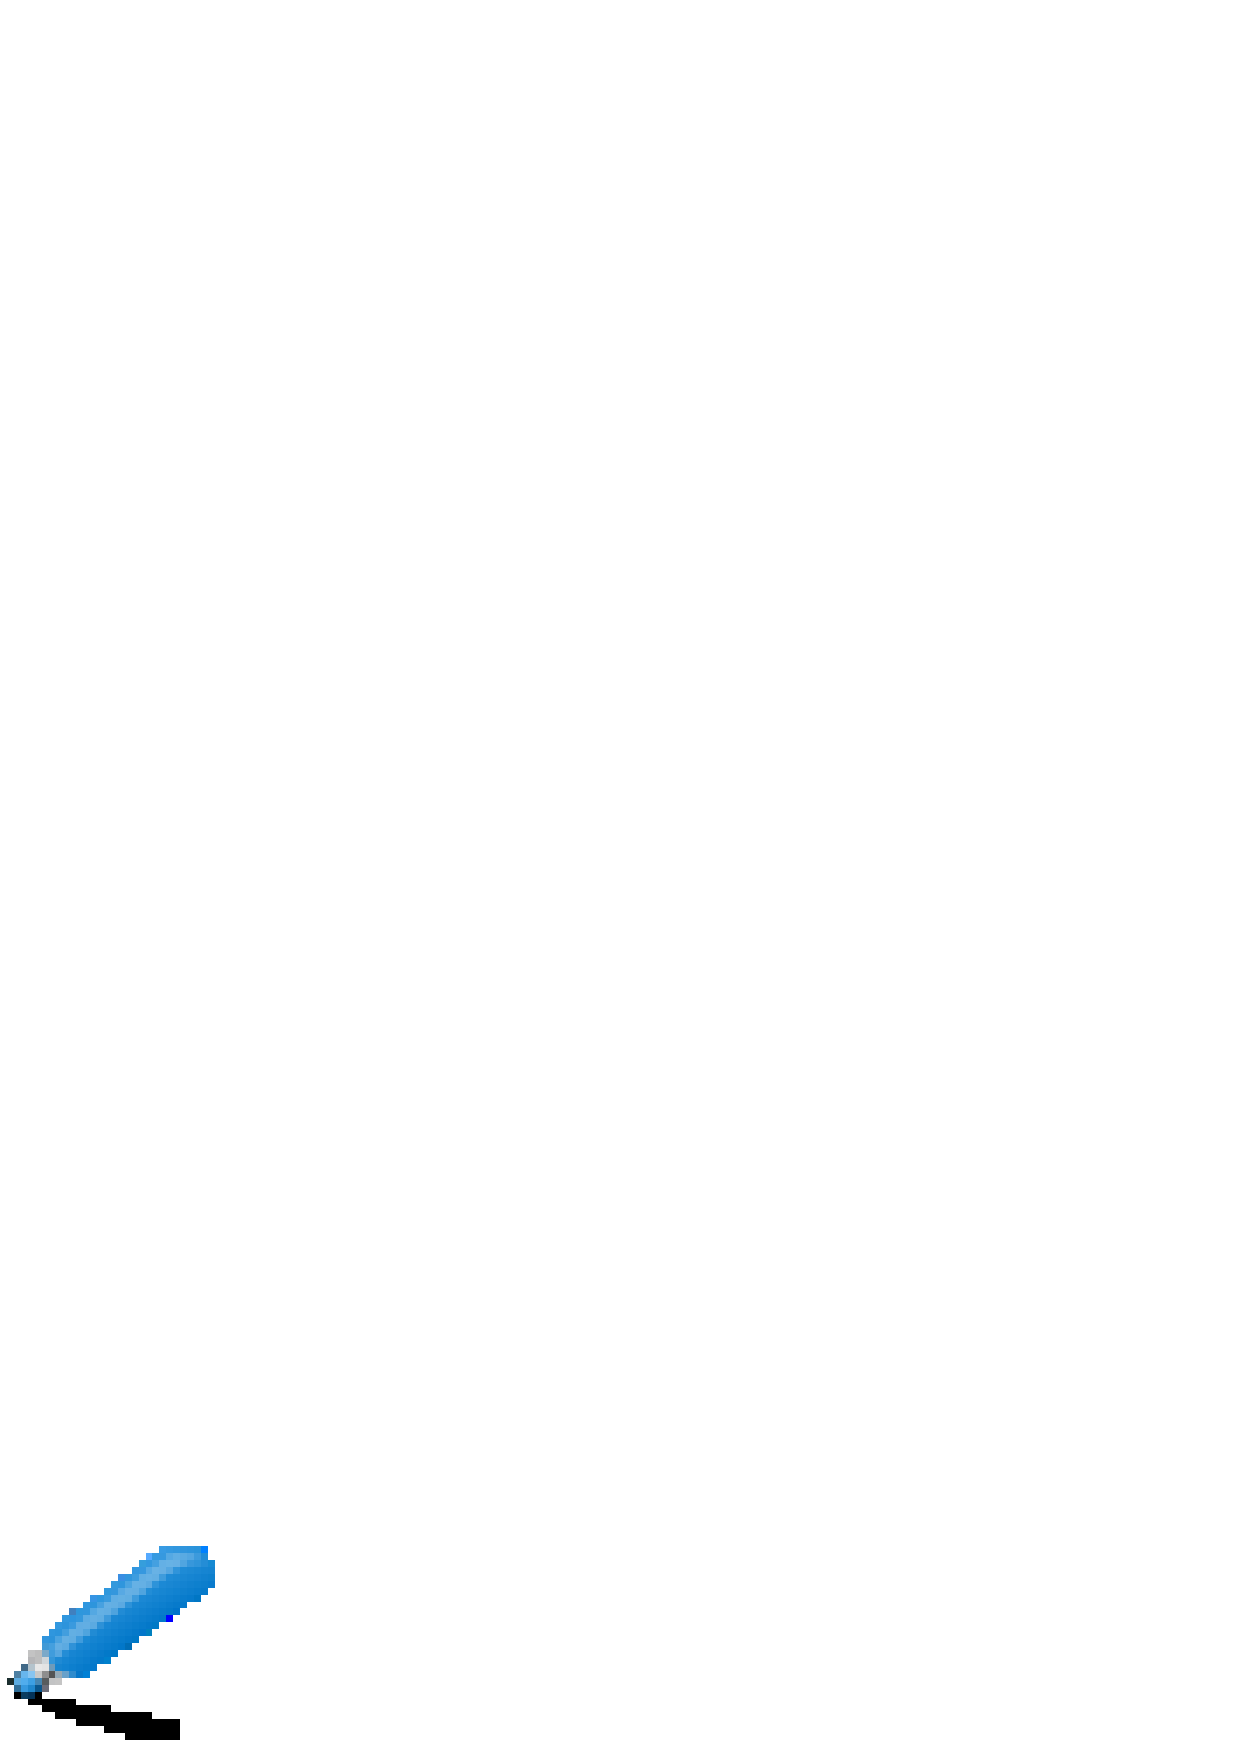
\includegraphics[width=0.7cm]{mActionToggleEditing}
   & Attiva modifica
   & 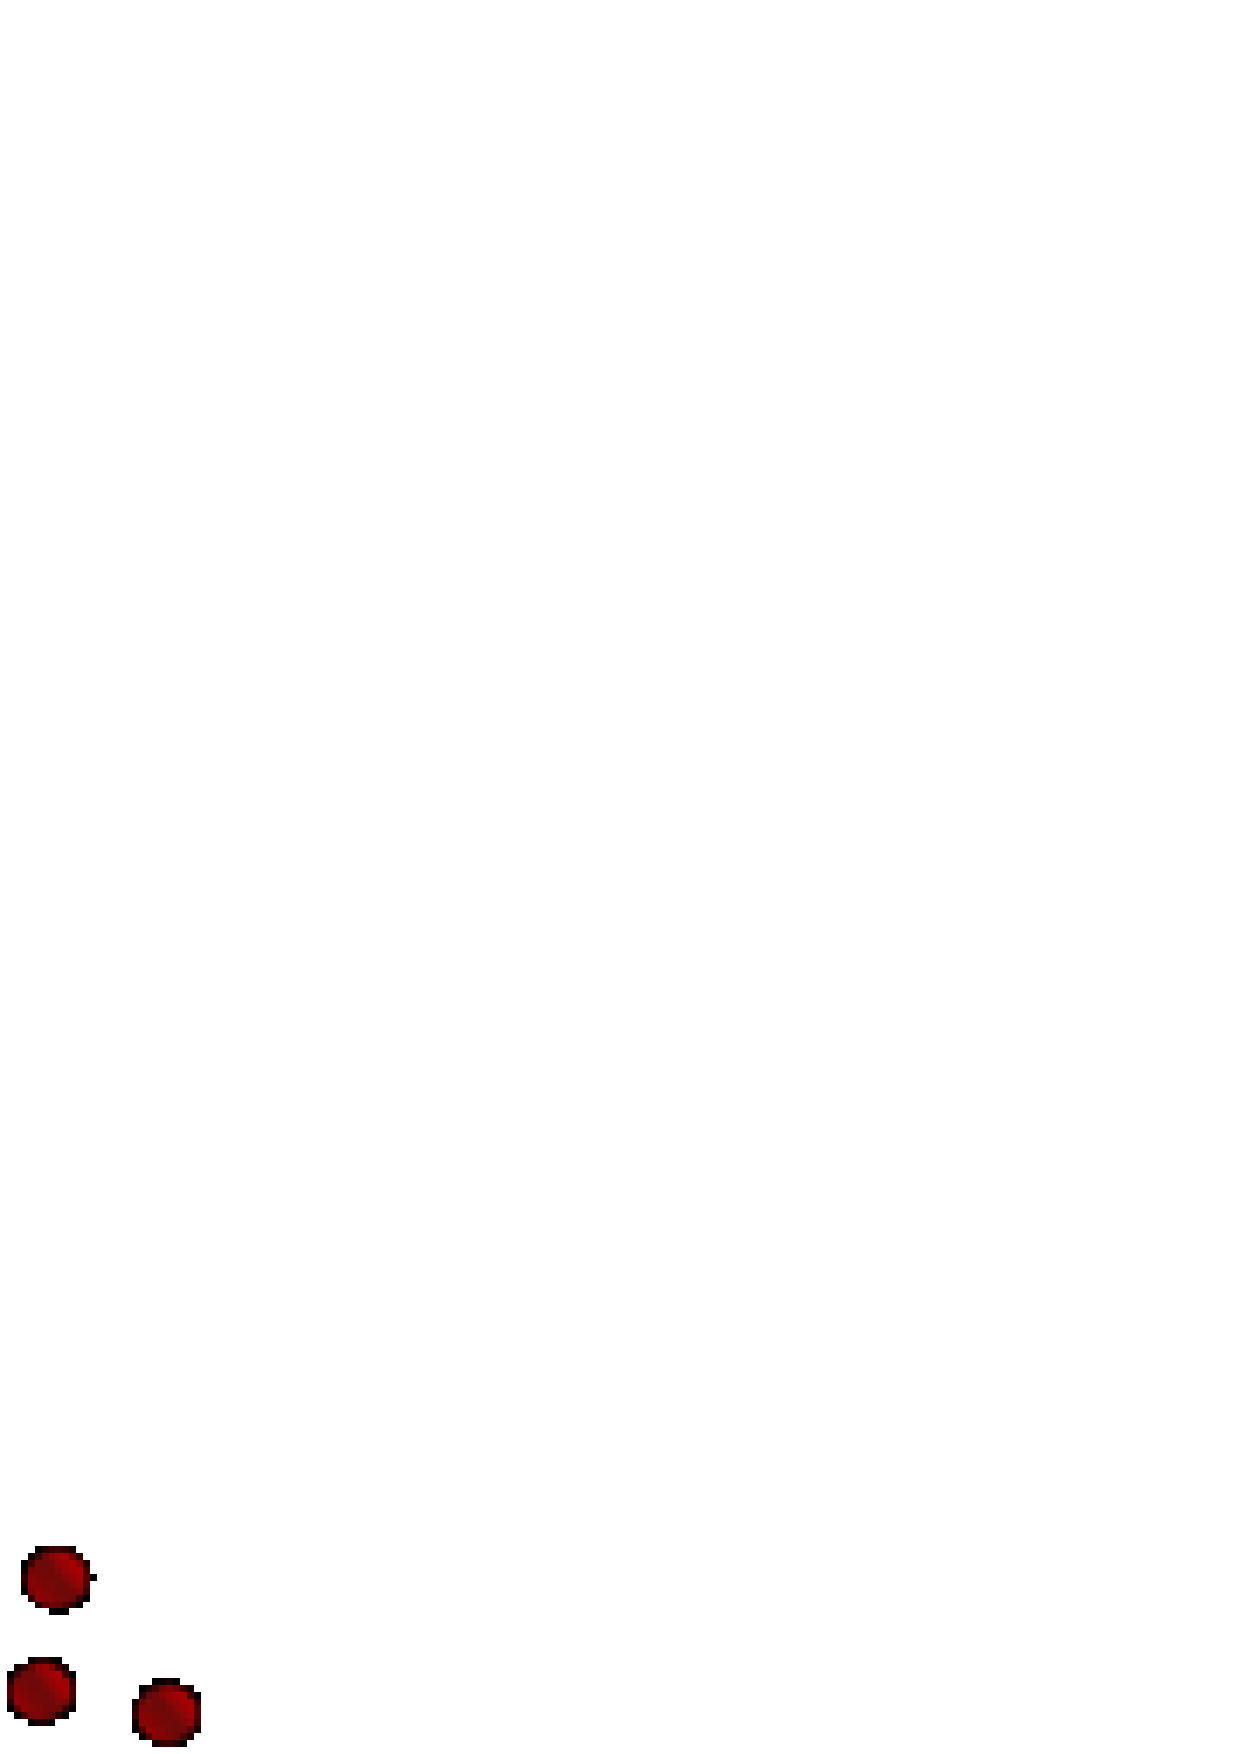
\includegraphics[width=0.7cm]{mActionCapturePoint}
   & Aggiunge elementi: Inserisci punto \\
\hline 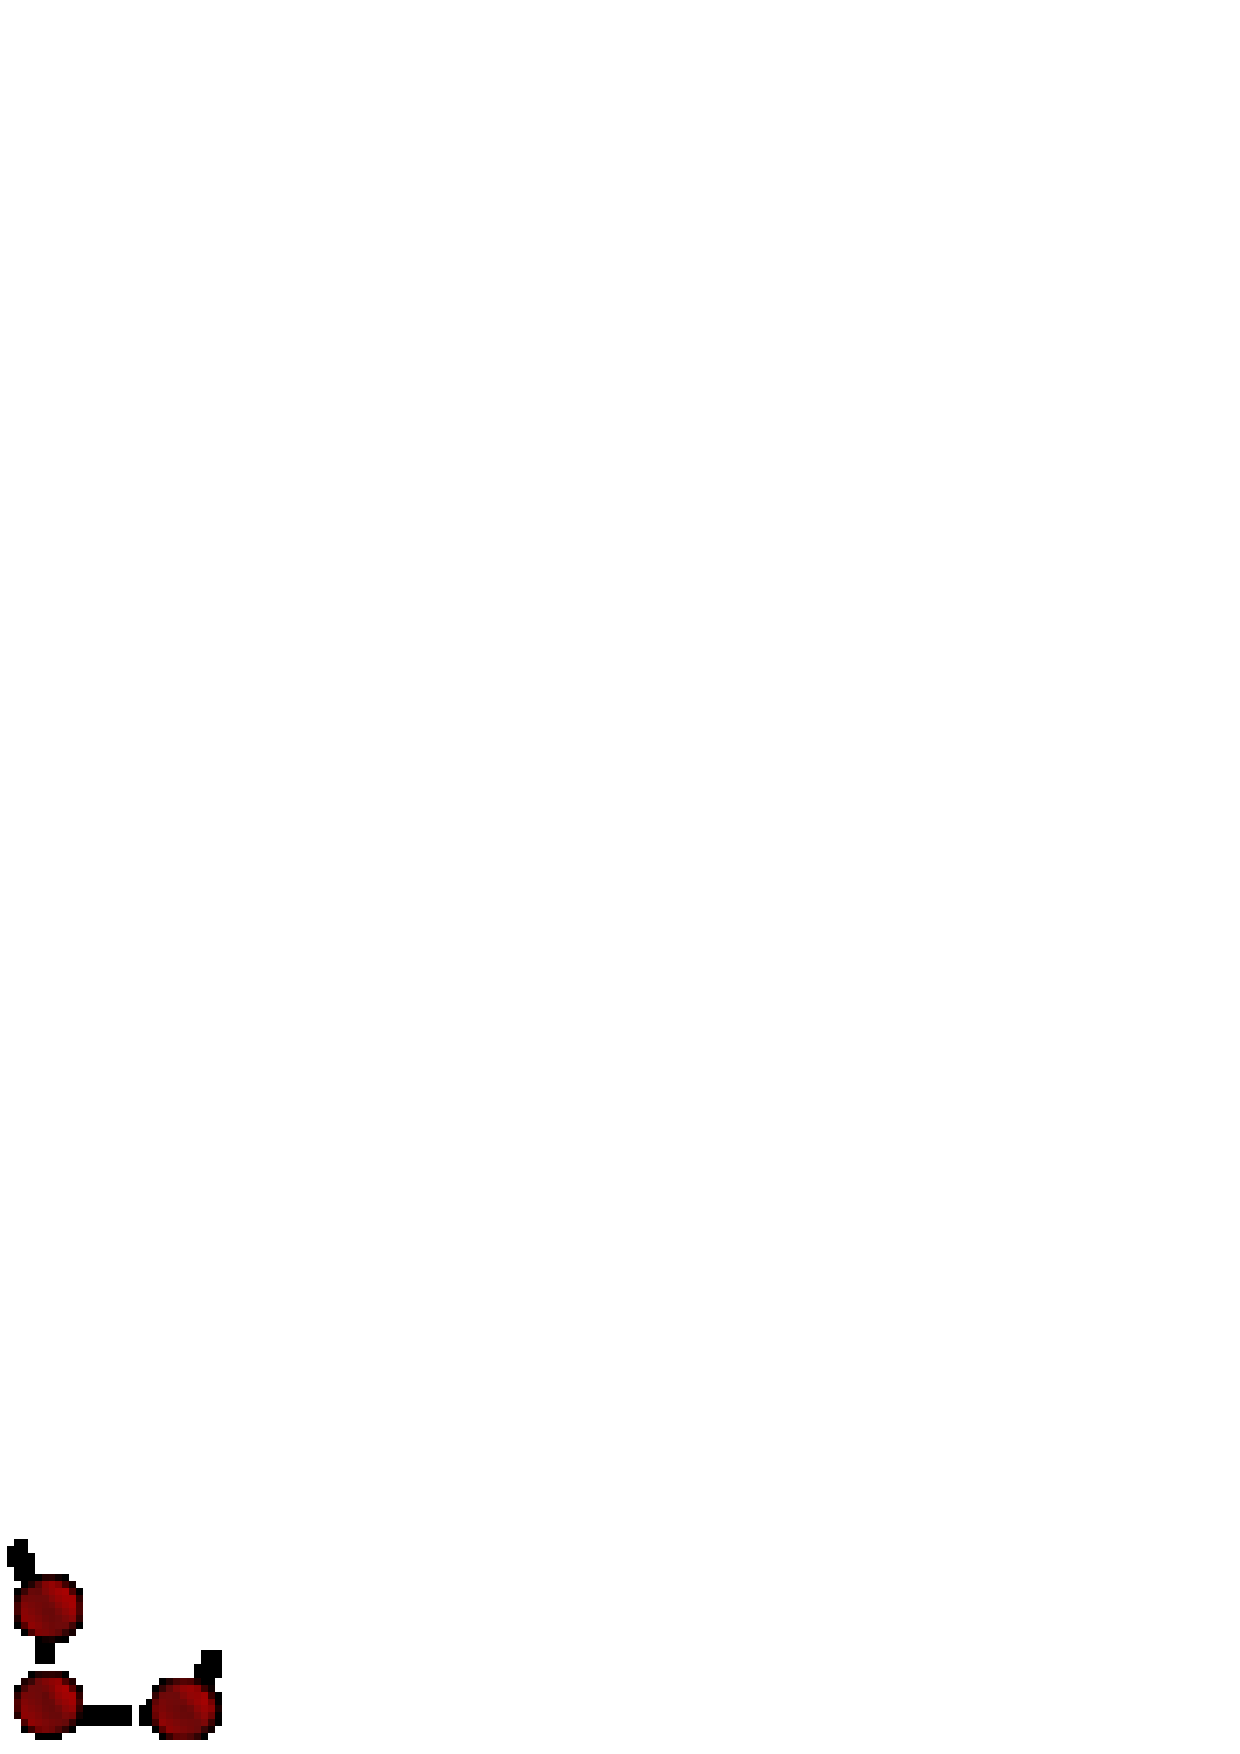
\includegraphics[width=0.7cm]{mActionCaptureLine}
   & Aggiunge elementi: Inserisci linea 
   & 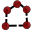
\includegraphics[width=0.7cm]{mActionCapturePolygon}
   & Aggiunge elementi: Inserisci poligono  \\
\hline 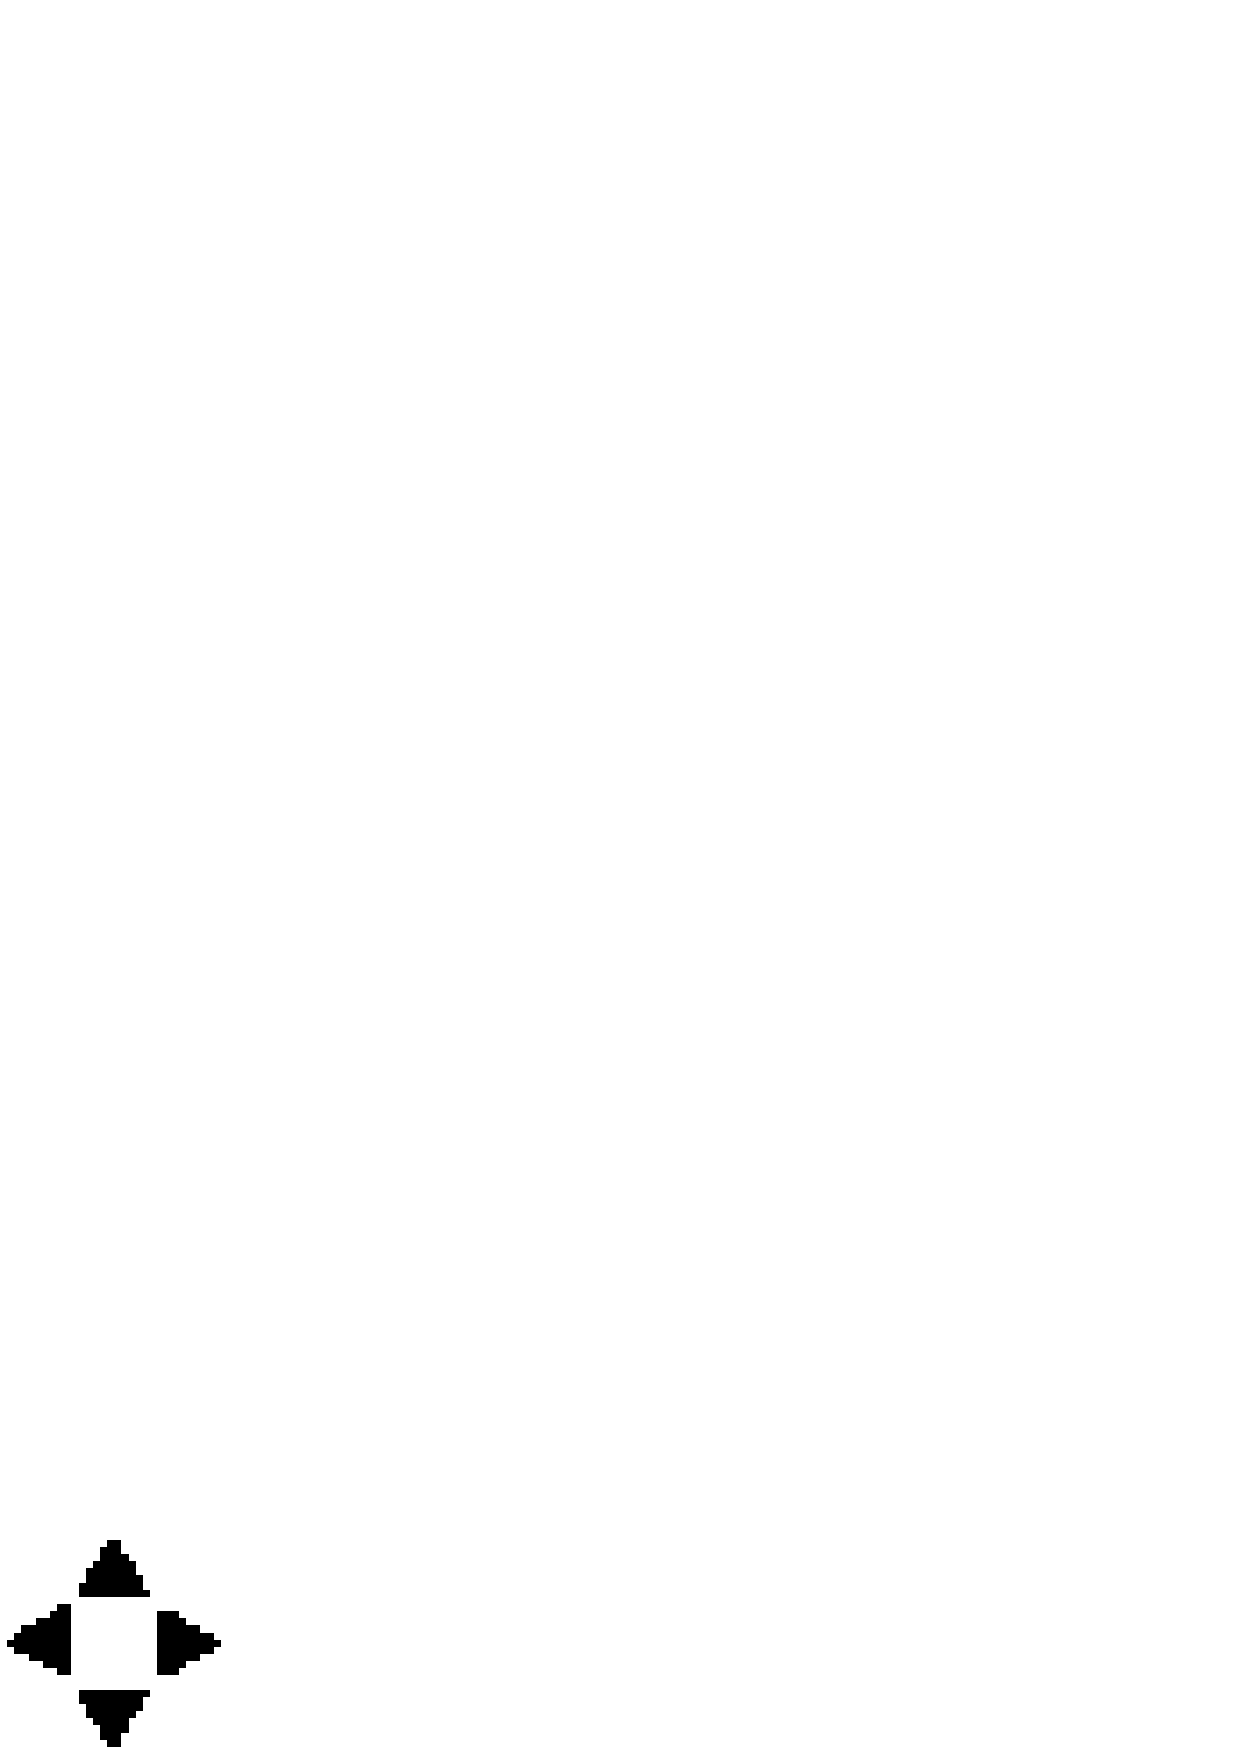
\includegraphics[width=0.7cm]{mActionMoveFeature}
   & Muove elementi
   & 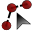
\includegraphics[width=0.7cm]{mActionNodeTool}
   & Strumento vertici \\
\hline 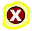
\includegraphics[width=0.7cm]{mActionDeleteSelected}
   & Elimina elementi selezionati
   & 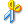
\includegraphics[width=0.7cm]{mActionEditCut}
   & Taglia elementi \\
\hline 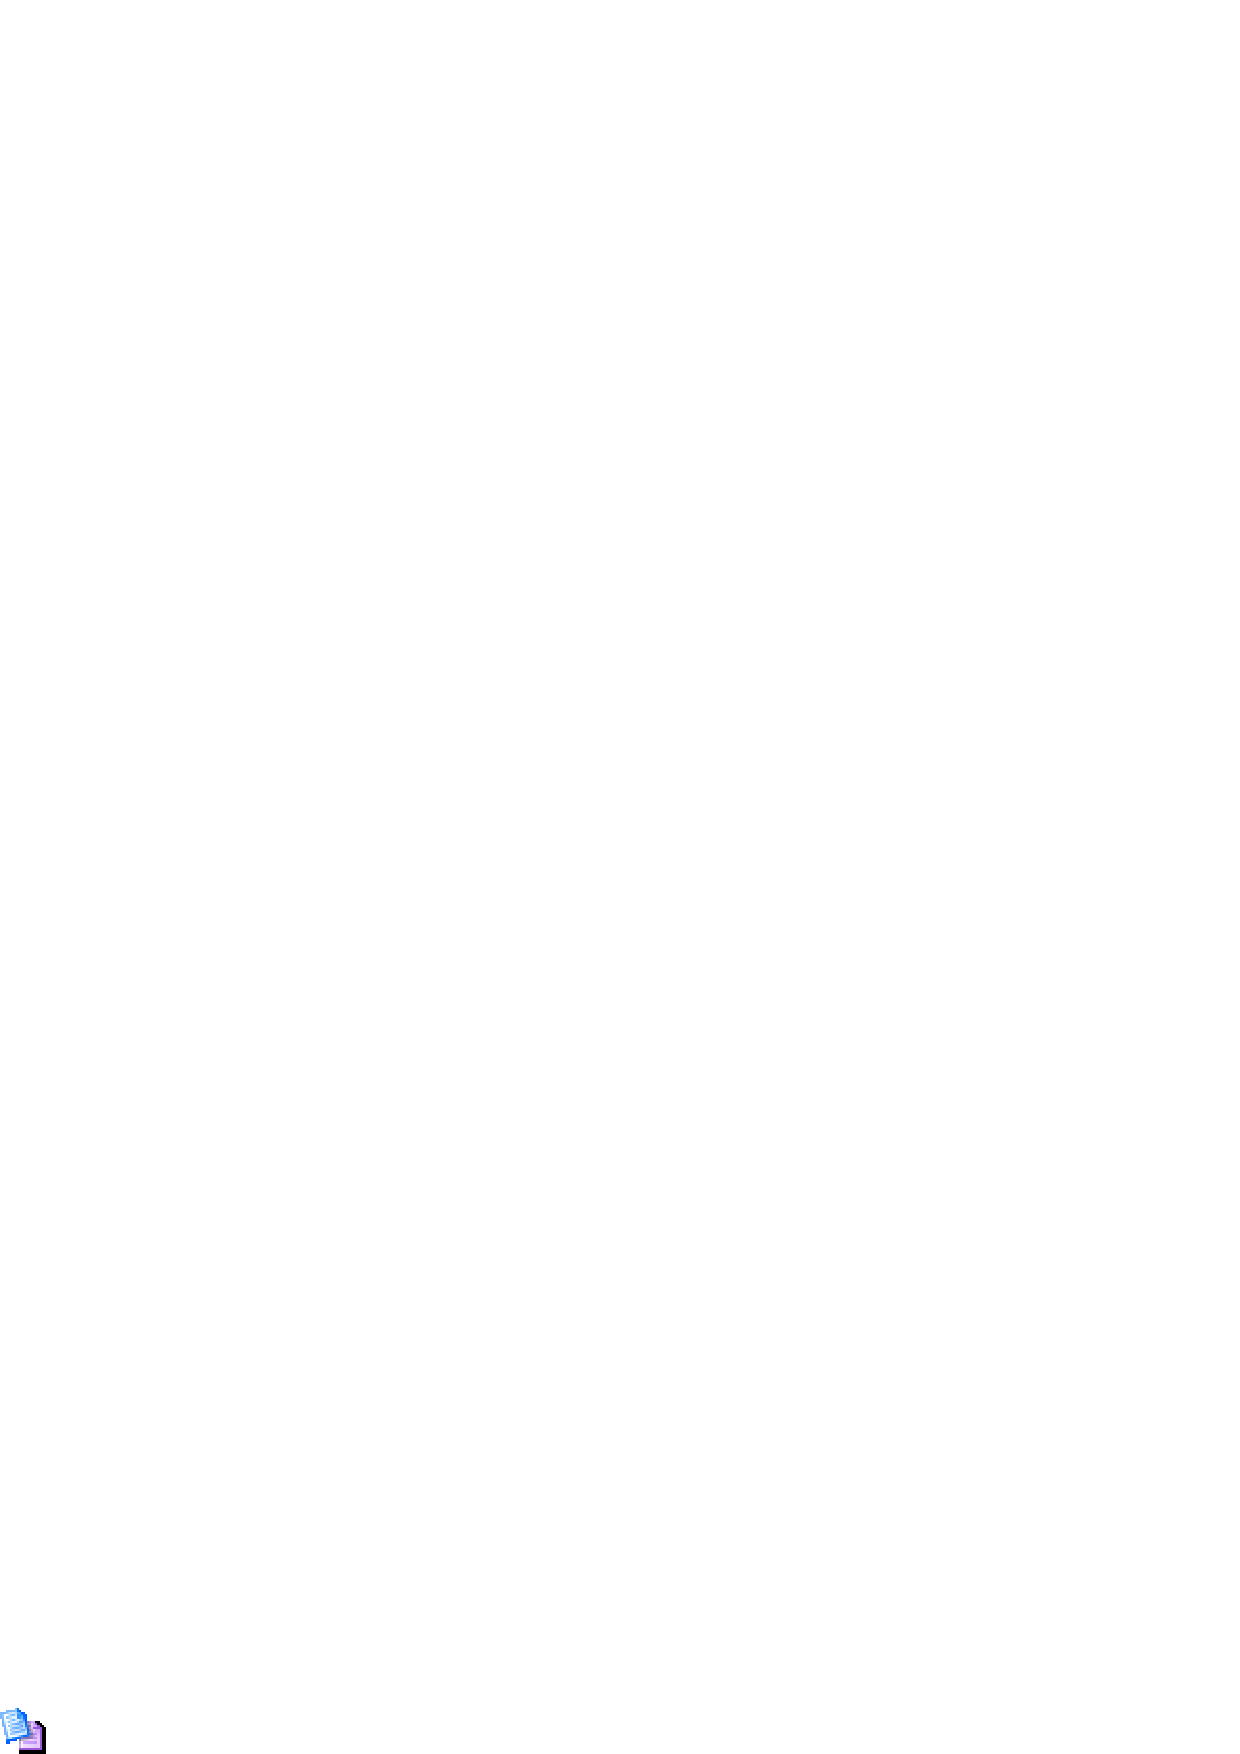
\includegraphics[width=0.7cm]{mActionEditCopy}
   & Copia elementi 
   & 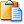
\includegraphics[width=0.7cm]{mActionEditPaste}
   & Incolla elementi \\
\hline 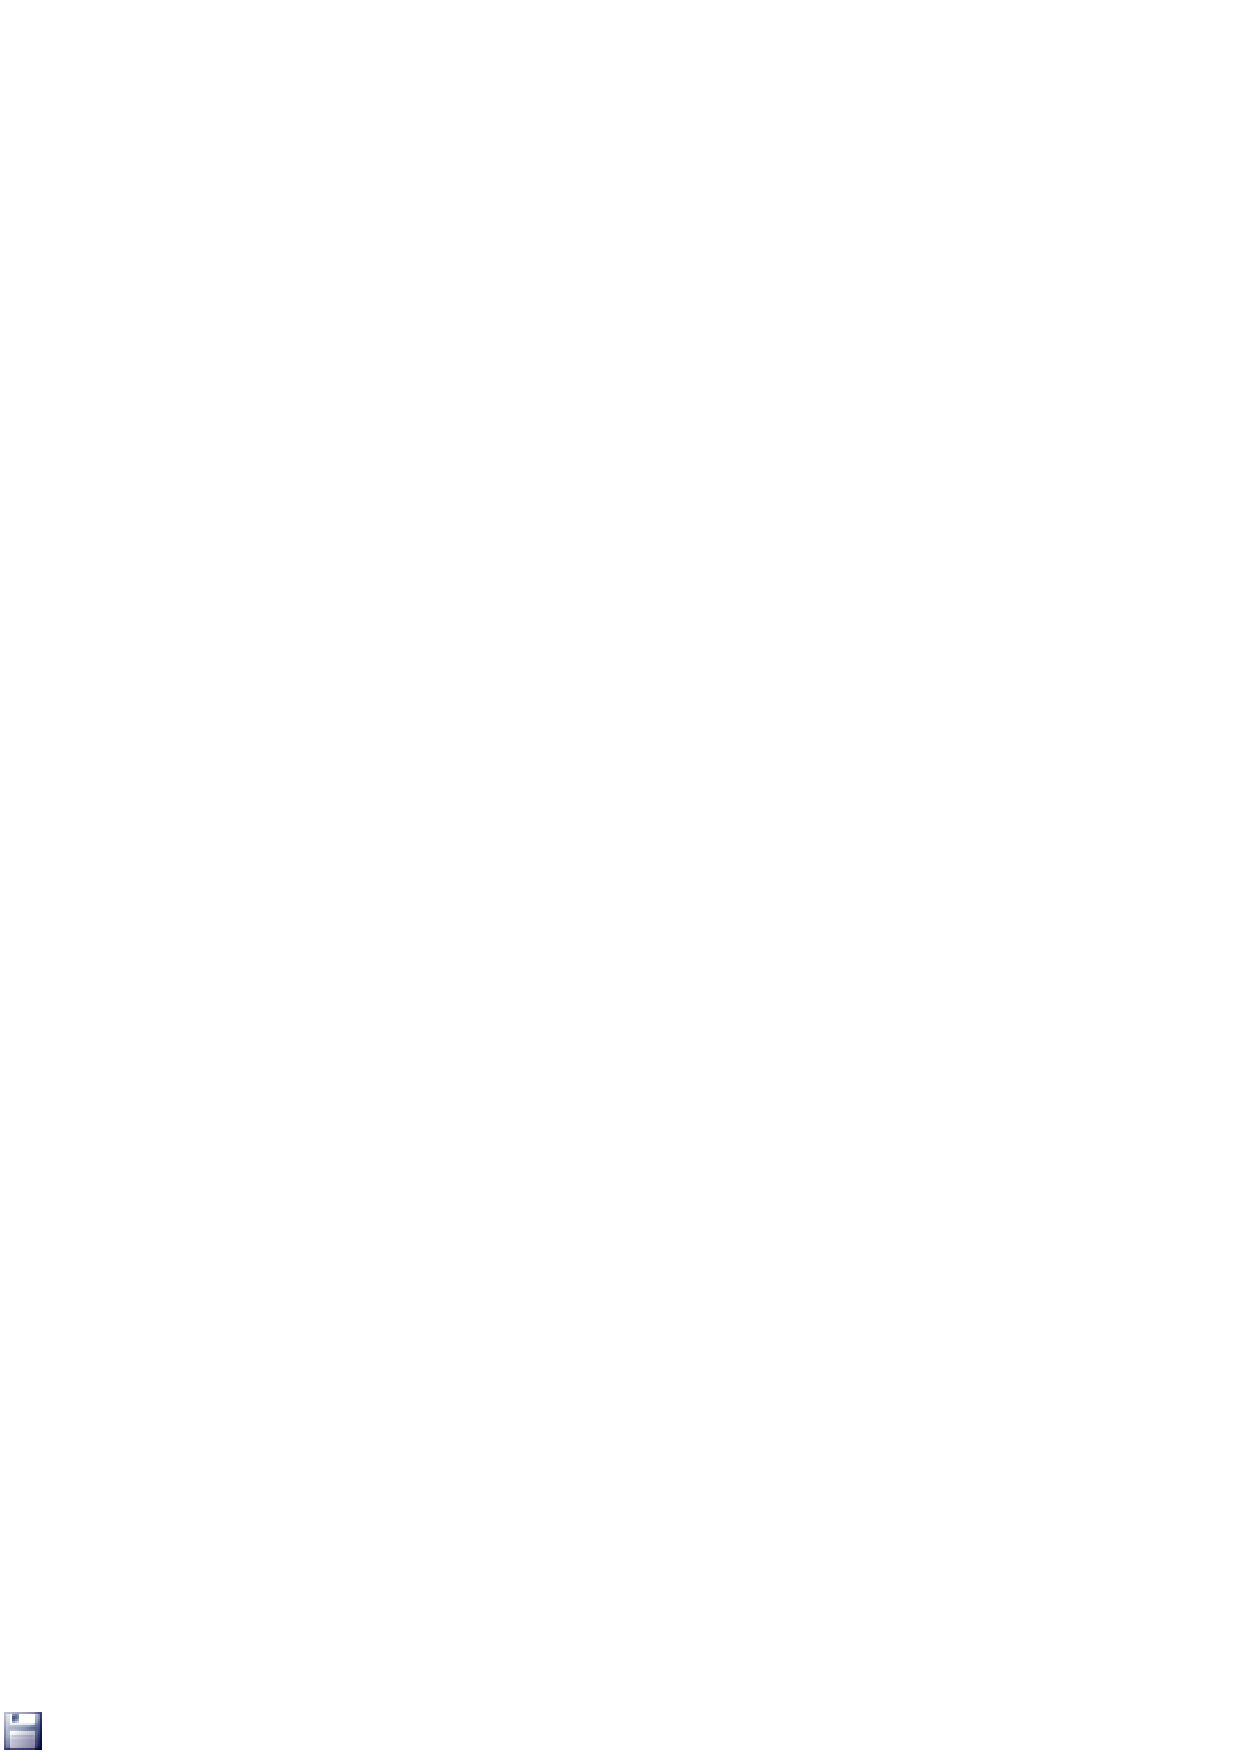
\includegraphics[width=0.7cm]{mActionFileSave}
   & Salva modifiche
   &  &  \\
\hline
\end{tabular}
\caption{Strumenti di base per la modifica di layer vettoriali}\label{tab:vector_editing}\medskip
\end{table}

Ogni sessione di modifica è inizializzata dall'opzione
\dropmenuopttwo{mActionToggleEditing}{Modifica}, che può
essere attivata e disattivata nel menù contestuale che si apre 
cliccando con il tasto destro del mouse sul nome del layer nella legenda. \index{attiva/disattiva modifica} 

In alternativa, è possibile usare il pulsante \index{attiva/disattiva modifica} 
\toolbtntwo{mActionToggleEditing}{Modifica}.\index{modifica!icone} 
Quando il layer è in modalità modifica, i vertici sono contrassegnati da indicatori (croci o cerchi
semitrasparenti) e altri strumenti sono attivati nella barra degli strumenti di modifica.

\begin{Tip}\caption{\textsc{Salvataggio ad intervalli regolari}}
Ricordarsi di usare \toolbtntwo{mActionFileSave}{Salva modifiche} regolarmente, in modo da
consentire il salvataggio delle modifiche recenti e per verificare che le stesse siano accettate 
dalla fonte di dati.
\end{Tip}

\minisec{Aggiungere elementi}
\index{layer vettoriali!aggiungere!elemento}
\index{layer vettoriali!muovere!elemento}

È possibile usare gli strumenti \toolbtntwo{mActionCapturePoint}{Inserisci punto},
\toolbtntwo{mActionCaptureLine}{Inserisci linea} o
\toolbtntwo{mActionCapturePolygon}{Inserisci poligono} per porre il puntatore
di QGIS in modalità digitalizzazione.

Per ogni elemento, bisogna dapprima digitalizzare la geometria e
successivamente inserire gli attributi. Per digitalizzare la geometria, cliccare 
con il tasto sinistro del mouse nella vista mappa per creare il primo punto del nuovo elemento.

Per linee e poligoni, continuare a cliccare con il tasto sinistro per ogni
ulteriore vertice che si desidera inserire. Quando è terminato l'inserimento
dei vertici o dei punti, cliccare con il tasto destro in qualunque punto della
mappa per confermare di aver terminato l'inserimento della geometria dell'elemento.

Apparirà quindi la finestra degli attributi che consentirà di inserire le
informazioni per l'elemento appena creato (Figura \ref{fig:vector_digitising}).
Nella scheda \tab{Digitalizzazione} della voce di menu \mainmenuopt{Impostazioni} \arrow \dropmenuopt{Opzioni}, 
è possibile attivare/disattivare le due opzioni:
\\
\checkbox{Non aprire la finestra degli attributi dopo la creazione di ogni geometria} \\
\checkbox{Ripeti i valori degli attributi usati per ultimi}.

\begin{figure}[ht]
   \centering
   \includegraphics[clip=true, width=8cm]{editDigitizing}
   \caption{Finestra di inserimento degli attributi per un elemento di nuova
   digitalizzazione \nixcaption}\label{fig:vector_digitising}
 \end{figure}

Per spostare degli elementi utilizzare lo strumento \toolbtntwo{mActionMoveFeature}{Muovi elemento/i}

\begin{Tip}\caption{\textsc{Tipologie di attributo}}
Relativamente agli shapefile, la modifica del tipo di attributo è validata durante
l'inserimento, per cui non è ovviamente possibile inserire un numero in una colonna testuale 
quando compare la finestra di dialogo \dialog{Attributi} e viceversa. Qualora si avesse tale necessità, 
è necessario modificare gli attributi in un secondo momento per mezzo della finestra di dialogo 
\dialog{Tabella degli attributi}.
\end{Tip}

\minisec{Modificare i vertici di un elemento}
\index{layer vettoriali!modificare!vertice}

Sia per i layer PostgreSQL/PostGIS che per gli shapefile, lo \toolbtntwo{mActionNodeTool}{Strumento vertici} 
fornisce capacità di modifica dei vertici simili ai programmi CAD. È possibile selezionare più vertici
contemporaneamente e spostarli e/o cancellarli con un'unica operazione. Lo strumento supporta la modifica 
topologica e lavora anche con la proiezione al volo attiva; se non trova nessun elemento apre una finestra 
di avviso che suggerisce di controllare le impostazioni di snapping. Pertanto, è importante impostare 
\mainmenuopt{Impostazioni} \arrow \dropmenuopttwo{mActionOptions}{Opzioni} \arrow \tab{Digitalizzazione} 
\arrow \selectnumber{Raggio di ricerca per le modifiche dei vertici}{10} ad un valore superiore a 0, 
altrimenti \qg non è in grado di gestire adeguatamente la modifica dei vertici.

\begin{Tip}\caption{\textsc{Indicatori dei vertici}}
La versione di QGIS attuale supporta tre tipi di indicatori per i vertici (in
modalità modifica): un cerchio semitrasparente, una croce o nulla. Per cambiare lo stile dell'indicatore,
scegliere la voce \dropmenuopttwo{mActionOptions}{Opzioni} dal menu \mainmenuopt{Impostazioni}, 
cliccare sulla scheda \tab{Digitalizzazione} e selezionare lo stile indicatore preferito.
\end{Tip}

\minisec{Operazioni di base}\index{layer vettoriali!Strumento vertici}

Attivare lo strumento \toolbtntwo{mActionNodeTool}{Strumento vertici} e selezionare un elemento 
cliccandoci sopra: un riquadro rosso apparirà su ogni vertice dell'elemento.
Si noti che per selezionare un poligono bisogna cliccare uno dei suoi vertici e dei suoi lati; 
cliccare all'interno del poligono produce un errore. Una volta selezionato un elemento, sono 
possibili le seguenti azioni: 

\begin{itemize}[label=--]
\item \textbf{Selezionare vertici}: per selezionare vertici è possibile cliccare su di essi, 
cliccare su un bordo per selezionare i vertici ai due estremi dello stesso, tracciare un 
riquadro intorno ai vertici di interesse. Il colore di un vertice selezionato passa dal rosso 
al blu. Per aggiungere ulteriori vertici a quelli già selezionati, cliccare sugli stessi tenendo 
contemporaneamente premuto il tasto \keystroke{Ctrl}. Per cambiare lo stato di un vertice 
(selezionato/non selezionato) cliccare lo stesso tenendo premuto contemporaneamente il tasto 
\keystroke{Ctrl}\keystroke{Shift}
\item \textbf{Aggiungere vertici}: per aggiungere un vertice fare doppio click nei pressi di un 
bordo. Si noti che il vertice apparirà sul bordo e non alla posizione del cursore del mouse.
\item \textbf{Eliminare vertici}: per eliminare un vertice selezionato basta premere il tasto
\keystroke{Canc}. Si noti che non è possibile eliminare un intero elemento tramite lo strumento 
\toolbtntwo{mActionNodeTool}{Strumento vertici}; \qg manterrà un numero minimo di vertici per il 
tipo di elemento su cui si sta lavorando. Per eliminare completamente un elemento, usare lo strumento
\toolbtntwo{mActionDeleteSelected}{Elimina il selezionato}.
\item \textbf{Spostare vertici}: selezionare i vertici di interesse, quindi cliccare e trascinare nella
direzione verso la quale si intende spostare i vertici; i vertici saranno spostati tutti insieme. 
Se lo snap è attivo, l'intera selezionare può essere agganciata al vertice e/o linea più vicina.
\end{itemize}

Ogni cambiamento operato con lo strumento vertici è memorizzato nel dialogo Annulla. Tutte le operazioni 
supportano le modifiche topologiche (se attivate) ed è possibile operare con la proiezione a volo attiva.
Lo strumento vertici offre, inoltre, la possibilità di ottenere informazioni su un vertice lasciando semplicemente 
il cursore del mouse sul vertice di interesse.

\minisec{Tagliare, copiare ed incollare elementi}
\index{layer vettoriali!tagliare!elemento}
\index{layer vettoriali!copiare!elemento}
\index{layer vettoriali!incollare!elemento}
\index{modifica!tagliare elementi}
\index{modifica!copiare elementi}
\index{modifica!incollare elementi}

Gli elementi selezionati possono essere tagliati, copiati ed incollati
tra layer dello stesso progetto di \qg a patto che anche per il layer di destinazione
sia stata abilitata la modalità di modifica tramite l'opzione 
\toolbtntwo{mActionToggleEditing}{Modifica}.

Gli elementi possono essere anche incollati in applicazioni esterne in formato testo: gli 
elementi verranno rappresentati nel formato CSV con le informazioni della geometria 
espresse nel formato testo OGC Well-Known Text (WKT).

Tuttavia in questa versione di \qg elementi di testo formattato creati con
applicazioni esterne non possono essere incollate in un layer vettoriale.

Le funzioni di copia/incolla sono utili quando si devono modificare più 
layer copiando le modifiche effettuate in uno di questi negli altri. 
Supponendo, ad esempio, di voler lavorare su un layer contenente solo alcuni
laghi, diventa molto più agevole creare un nuovo layer vuoto nel quale
incollare gli elementi dei quali necessitiamo invece di lavorare sul layer 
\filename{big\_lakes} contenente 5000 elementi. 

Dovremo quindi effettuare le seguenti operazioni:

\begin{enumerate}
\item Caricare il layer dal quale vogliamo copiare gli elementi (layer
sorgente)
\item Caricare o creare il layer nel quale vogliamo incollare gli elementi
copiati (layer di destinazione) 
\item Impostare entrambi i layer in modalità modifica 
\item Rendere attivo il layer sorgente cliccando sul relativo nome nella
legenda 
\item Attivare lo strumento \toolbtntwo{mActionSelect}{Seleziona il singolo elemento}
per selezionare gli elementi dal layer sorgente
\item Cliccare sullo strumento \toolbtntwo{mActionEditCopy}{Copia elementi}
\item Rendere attivo il layer di destinazione cliccando sul relativo nome
nella legenda
\item Attivare lo strumento \toolbtntwo{mActionEditPaste}{Incolla elementi} 
\item Terminare le modifiche e salvare
\end{enumerate}

Se il layer sorgente e quello di destinazione hanno un diverso schema (nomi e
tipi dei campi) \qg popola, se presenti, i campi comuni e ignora il resto.
Se non è importante che vengano copiati anche gli attributi nel layer di
destinazione, si può non prestare attenzione a come viene definito lo schema
della tabella attributi, altrimenti è necessario definirlo in modo che 
lo schema del layer sorgente e quello del layer di destinazione combacino.

\begin{Tip}\caption{\textsc{Congruenza degli elementi incollati}}
Se il layer sorgente e quello di destinazione usano lo stesso sistema
di proiezione, gli elementi incollati saranno assolutamente identici a quelli
del layer di origine. Nel caso in cui invece la proiezione del layer di
destinazione sia differente  \qg non garantisce che la geometria sia identica
a causa del pur ridotto errore di arrotondamento introdotto nel passaggio da
un sistema di proiezione all'altro.
\end{Tip}

\minisec{Cancellare elementi selezionati}
\index{layer vettoriali!cancellare!elemento}

Se si vuole eliminare un intero poligono, è possibile farlo selezionando
dapprima l'elemento che intendiamo cancellare con lo strumento
\toolbtntwo{mActionSelect}{Seleziona il singolo elemento}: è possibile anche 
selezionare più poligoni contemporaneamente. Una volta definita la selezione, 
usare lo strumento \toolbtntwo{mActionDeleteSelected}{Elimina il selezionato} 
per cancellare la selezione. 

Anche lo strumento \toolbtntwo{mActionEditCut}{Taglia geometrie} può essere
usato per eliminare elementi: tali elementi vengono spostati in un
"blocco appunti spaziale". In questo modo è possibile annullare
l'operazione incollando nuovamente gli elementi tagliati con lo strumento
\toolbtntwo{mActionEditPaste}{Incolla elementi}, fornendo in ultima
analisi almeno un livello di annullamento.
Gli strumenti taglia, copia e incolla lavorano sugli elementi selezionati, 
consentendo quindi di lavorare su più di un elemento alla volta.

\begin{Tip}\caption{\textsc{Supporto alla cancellazione di elementi}}
Quando si modificano shapefile, la cancellazione di elementi funziona solo se 
\qg è compilato con una versione di GDAL pari a 1.3.2 o
superiore, come accade per le versioni compilate per OS X e Windows
disponibili sul sito.
\end{Tip}

\minisec{Salvare i layer modificati}
\index{modifica!salvare modifiche}

Quando un layer è in modalità modifica, tutti i cambiamenti rimangono nella
memoria di \qg e quindi non sono immediatamente applicati e salvati nei dati
su disco. Se si vogliono salvare le modifiche di un layer senza abbandonare la
modalità modifica è possibile utilizzare lo strumento \toolbtntwo{mActionFileSave}{Salva modifiche}.
Quando viene disabilitata la modalità di modifica con \toolbtntwo{mActionToggleEditing}{Modifica} 
(o si termina la sessione di \qg mentre questa non è stata finalizzata), 
viene chiesto se si desidera salvare o scartare le modifiche.

Se le modifiche non possono essere salvate (ad es. perché il disco di
destinazione è pieno o gli attributi contengono valori esterni agli estremi
ammissibili), lo stato della memoria di \qg è preservato, consentendo dunque
di correggere gli errori e riprovare il salvataggio.

\begin{Tip}\caption{\textsc{Integrità dei dati}}
È buona norma fare un back-up del dato originale prima di procedere
alla modifica. Per quando siano stati fatti molti sforzi da parte dei
programmatori di QGIS per preservare l'integrità del dato, non vi è alcuna
garanzia che ciò avvenga.
\end{Tip}

\subsection{Digitalizzazione avanzata}
\index{layer vettoriali!digitalizzazione avanzata}
\index{digitalizzazione avanzata!layer esistente}
\label{sec:advanced_edit}

\begin{table}[h]\index{layer vettoriali!strumenti di digitalizzazione avanzata}
\centering
\small
\begin{tabular}{|l|p{6.9cm}|l|p{6.9cm}|}
\hline \textbf{Icona} & \textbf{Azione} & \textbf{Icona} & \textbf{Azione} \\
\hline \includegraphics[width=0.7cm]{mActionUndo}
   & Annulla
   & \includegraphics[width=0.7cm]{mActionRedo}
   & Ripristina \\
\hline \includegraphics[width=0.7cm]{mActionSimplify}
   & Semplifica geometrie
   & \includegraphics[width=0.7cm]{mActionAddRing}
   & Aggiungi buco \\
\hline \includegraphics[width=0.7cm]{mActionAddIsland}
   & Aggiungi una parte
   & \includegraphics[width=0.7cm]{mActionDeleteRing}
   & Elimina buco \\
\hline \includegraphics[width=0.7cm]{mActionDeletePart}
   & Elimina parte
   & \includegraphics[width=0.7cm]{mActionReshape}
   & Modifica la forma \\
\hline \includegraphics[width=0.7cm]{mActionSplitFeatures}
   & Spezza elemento
   & \includegraphics[width=0.7cm]{mActionMergeFeatures}
   & Unisce le geometrie selezionate \\
\hline \includegraphics[width=0.7cm]{mActionMergeFeatures}
   & Unisce gli attributi delle geometrie selezionate
   &\includegraphics[width=0.7cm]{mActionRotatePointSymbols}
   & Ruota i simboli per i punti \\
\hline
\end{tabular}
\caption{Barra degli strumenti di digitalizzazione avanzata}\label{tab:advanced_editing}
\end{table}

\minisec{Annullare e ripristinare}
\index{layer vettoriali!annulla}
\index{layer vettoriali!ripristina}

Gli strumenti \toolbtntwo{mActionUndo}{Annulla} e \toolbtntwo{mActionRedo}{Ripristina} 
permettono di annullare/ripristinare le modifiche ad un layer vettoriale. Inoltre, è 
disponibile un widget che memorizza e mostra tutte le operazioni annulla/ripristina
(Figura \ref{fig:vector_redoundo}). Per attivare il widget cliccare con il tasto 
destro del mouse sulla barra degli strumenti ed attivare la casella di controllo 
Annulla/Ripristina. Annulla/Ripristina è comunque attivo, anche se il widget non è
visibile.

Cliccando su Annulla, tutti gli elementi e gli attributi vengono riportati al loro stato 
precedente. Le modifiche effettuate con strumenti diversi da quelli per la digitalizzazione
(es. un plugin), potrebbero non essere annullabili.

Se nel widget Annulla/Ripristina si clicca su una determinata operazione, tutti gli
elementi saranno riportati allo stato successivo all'operazione selezionata.

\begin{figure}[ht]
   \centering
   \includegraphics[clip=true, width=12cm]{redo_undo}
   \caption{Elenco delle operazioni nel widget Annulla/Ripristina \wincaption}\label{fig:vector_redoundo}
\end{figure}

\minisec{Semplificare una geometria}
\index{layer vettoriali!semplifica}

Lo strumento \toolbtntwo{mActionSimplify}{Semplifica geometrie} permette di ridurre il numero di 
vertici di un elemento, preservandone la geometria: un elemento selezionato con lo strumento 
sarà evidenziato da una linea di semplificazione rossa, inoltre verrà mostrato a schermo un cursore 
(Tolleranza linea di semplificazione). Muovendo il cursore, la linea di semplificazione cambia e 
mostra la forma che assumerà l'elemento che si sta semplificando. Per memorizzare la geometria 
semplificata, cliccare su \button{OK}.
Se una geometria non può essere semplificata (come nel caso di un multi-poligono), verrà mostrato un 
messaggio di errore.

\minisec{Aggiungere un buco}
\index{layer vettoriali!inserire!buco}

Si possono digitalizzare nuovi poligoni all'interno di poligoni esistenti, al fine
di creare un buco all'interno di questi ultimi, scegliendo lo strumento \toolbtntwo{mActionAddRing}{Aggiungi buco}.
In questo modo solo l'area compresa tra i bordi del poligono interno e di
quello esterno verrà  evidenziata come poligono ad anello. 

\minisec{Aggiungere una parte}
\index{layer vettoriali!aggiungi!parte}

Lo strumento \toolbtntwo{mActionAddIsland}{Aggiungi una parte} permette di aggiungere 
una parte ad un multi-poligono; la nuova parte va digitalizzata all'esterno del poligono 
selezionato.

\minisec{Eliminare un buco}
\index{layer vettoriali!elimina!buco}

Lo strumento \toolbtntwo{mActionDeleteRing}{Elimina buco} permette di eliminare un 
buco all'interno di un poligono. Lo strumento funziona esclusivamente con layer di poligoni. 
Nessuna azione viene effettuata se lo strumento viene usato sul bordo esterno di un poligono.
Prima di selezionare i vertici di un buco, impostare adeguatamente la tolleranza.

\minisec{Eliminare una parte}
\index{layer vettoriali!!elimina!parte}

Lo strumento \toolbtntwo{mActionDeletePart}{Elimina parte} permette di eliminare parti 
da geometrie multi-parte (multi-punto, multi-linea, multi-poligono); lo strumento non 
ha effetto sull'ultima parte aggiunta. Prima di selezionare i vertici di una parte, 
impostare adeguatamente la tolleranza.

\minisec{Modificare la forma}
\index{layer vettoriali!modificare!elemento}

Lo strumento \toolbtntwo{mActionReshape}{Modifica la forma} permette di modificare la 
forma di elementi a geometria lineare e poligonale tracciando una nuova linea: la porzione 
di elemento tra i due punti di intersezione con la nuova linea sarà rimpiazzata dalla 
forma di quest'ultima. Prestare particolare attenzione ad utilizzare lo strumento con 
i poligoni: limitarsi a piccole porzioni di poligono. La nuova forma non può intersecare 
più buchi, altrimenti si generano poligoni non validi. 

Per modificare, ad esempio, il bordo di un poligono basta cliccare un primo punto all'interno 
del poligono, cliccare un secondo punto all'esterno del poligono, tracciare il profilo 
della nuova forma, rientrare nel poligono e cliccare con il tasto destro del mouse per terminare 
l'operazione. Lo strumento aggiungerà automaticamente nuovi nodi laddove la nuova linea 
interseca il bordo del poligono.

È, inoltre, possibile rimuovere parte di un poligono iniziando la nuova linea all'esterno del 
poligono, aggiungendo vertici all'interno e terminando la linea all'esterno con il 
tasto destro del mouse.

\textbf{Nota}: lo strumento potrebbe alterare la posizione iniziale di un poligono o di una
linea chiusa, per cui nodo iniziale e nodo finale potrebbero non coincidere. Per molte applicazioni
tale fatto non è un problema rilevante, ma è opportuno tenerne conto.

\minisec{Dividere elementi}
\index{layer vettoriali!spezzare!elementi}

È possibile dividere degli elementi tramite lo strumento \toolbtntwo{mActionSplitFeatures}{Spezza
elemento} e tracciando una linea attraverso l'elemento di interesse. 

\minisec{Unire elementi}
\index{layer vettoriali!spezzare!elementi}

Lo strumento \toolbtntwo{mActionMergeFeatures}{Unisci le geometrie selezionate} permette 
di unire elementi con bordi condivisi e stessi attributi.

\minisec{Unire attributi di elementi}
\index{layer vettoriali!unire!attributi}

Lo strumento \toolbtntwo{mActionMergeFeatures}{Unisci gli attributi degli elementi selezionati} 
permette di unire gli attributi di elementi con bordi condivisi e stessi attributi senza però, 
unirne i bordi.

\minisec{Ruotare simboli puntuali}
\index{layer vettoriali!ruotare!simboli}

%% FIXME change, if support in new symbology is available, too
Attualmente lo strumento \toolbtntwo{mActionRotatePointSymbols}{Ruota i simboli per i punti} è 
supportato dalla sola simbologia di vecchia generazione. Esso permette di cambiare la rotazione
di un simbolo per punti qualora sia stata definita una colonna rotazione nella tabella degli 
attributi di un layer puntuale (scheda \tab{Stile} della finestra di dialogo \dialog{Proprietà layer}). 
In caso contrario lo strumento non è attivo.

\begin{figure}[ht]
   \centering
   \includegraphics[clip=true, width=6cm]{rotatepointsymbol}
   \caption{Ruota simboli per punti \nixcaption}\label{fig:rotatepoint}
\end{figure}

Per modificare la rotazione, selezionare un elemento puntuale nella vista mappa e ruotarlo 
tenendo premuto il tasto sinistro del mouse; apparirà una freccia rossa ed il valore di 
rotazione (Figura~\ref{fig:rotatepoint}). Al termine dell'operazione, il valore di rotazione
nella tabella degli attributi sarà aggiornato di conseguenza.

\textbf{Nota}: Se si tiene premuto il tasto \keystroke{Ctrl}, la rotazione avverrà per step di 15 gradi.

\minisec{Creare un nuovo Shapefile}\label{sec:create shape}\index{modifica!creare un nuovo shapefile}

Per creare un nuovo layer shapefile selezionare \button{Nuovo} \arrow
\toolbtntwo{mActionNewVectorLayer}{Nuovo layer shapefile} dal menu 
\mainmenuopt{Layer}. Apparirà la finestra di dialogo \dialog{Nuovo vettore} mostrata
in Figura \ref{fig:newvectorlayer}. Scegliere il tipo di geometria (Punto, Linea o Poligono) 
ed il sistema di riferimento (SR).

\begin{figure}[ht]
   \centering
   \includegraphics[clip=true, width=8cm]{editNewVector}
   \caption{Finestra di dialogo per la creazione di un nuovo layer shapefile \nixcaption}\label{fig:newvectorlayer}
\end{figure}

Si noti che \qg non supporta la creazione di elementi 2.5D (ad es. elementi
con coordinate XYZ) o il conteggio degli elementi. Ad oggi inoltre possono
essere creati solo shapefile. Il supporto per la creazione di layer OGR o
PostgreSQL sarà implementato in future versioni di \qg. 

Per completare la creazione del nuovo layer shapefile vanno specificati gli attributi,
definendone nome e tipo e cliccando su \button{Aggiungi alla lista degli attributi}. 
La colonna 'id' è aggiunta automaticamente da QGIS, ma può essere eliminata. 
Allo stato attuale sono supportati sono attributi \selectstring{Tipo}{Numeri decimali}, 
\selectstring{Tipo}{Numeri interi} e \selectstring{Tipo}{Testo}: in funzione del 
tipo di attributo è possibile definire larghezza e precisione. 

Una volta definiti gli attributi, cliccare su \button{OK} e assegnare un nome allo shapefile.
\qg aggiungerà automaticamente l'estensione \filename{.shp} al nome indicato.
Una volta creato il layer, lo stesso sarà aggiunto alla vista mappa e potrà essere
modificato come descritto alla precedente Sezione \ref{sec:edit_existing_layer}.

\minisec{Creare un nuovo layer SpatiaLite}\label{sec:create spatialite}\index{modifica!Creare un nuovo layer spatiaLite}

Per creare un nuovo layer spatialite selezionare \button{Nuovo} \arrow
\toolbtntwo{mActionNewVectorLayer}{Nuovo layer SpatiaLite} dal menu 
\mainmenuopt{Layer}. Apparirà la finestra di dialogo \dialog{Nuovo layer SpatiaLite} mostrata
in Figura \ref{fig:newspatialitelayer}.

\begin{figure}[ht]
   \centering
   \includegraphics[clip=true, width=8cm]{editNewSpatialite}
   \caption{Finestra di dialogo per la creazione di un nuovo layer SpatiaLite \nixcaption}\label{fig:newspatialitelayer}
\end{figure}

Selezionare un database Spatialite esistente o crearne uno nuovo tramite il pulsante 
\button{...} alla destra del campo 'Database'. Indicare un nome per il nuovo layer, definire
il tipo di layer ed il sistema di riferimento (EPSG SRID). Se richiesto, è possibile creare
una chiave primaria autoincrementale selezionando \checkbox{Crea una chiave primaria autoincrementale}.

Per definire la tabella degli attributi del nuovo layer, indicare nome e tipo 
dell'attributo desiderato e cliccare su \button{Aggiungi alla lista degli attributi},
quindi cliccare su \button{OK} per terminare l'operazione.
Una volta creato il layer, lo stesso sarà aggiunto alla vista mappa e potrà essere
modificato come descritto alla precedente Sezione \ref{sec:edit_existing_layer}.

La finestra di dialogo SpatiaLite permette di creare più file senza essere chiusa e 
riaperta ogni volta: cliccare su \button{Apply} invece che su \button{OK}.

\subsection{Lavorare con la tabella degli attributi}
\label{sec:attribute table}
\index{modifica!lavorare con la tabella degli attributi}

La tabella degli attributi mostra gli elementi di un layer. Ogni riga
nella tabella rappresenta un elemento ed ogni colonna un attributo.
Gli elementi possono essere cercati, selezionati, spostati e modificati.

Per aprire la tabella degli attributi di un layer vettoriale, rendere attivo il layer e 
selezionare l'opzione \dropmenuopttwo{mActionOpenTable}{Apri tabella attributi}
dal menu \mainmenuopt{Layer}. Lo stesso risultato si ottiene cliccando con il
tasto destro del mouse sopra il layer in legenda e selezionando \dropmenuopttwo{mActionOpenTable}{Apri tabella attributi} 
dal menu contestuale. 
Si aprirà la finestra di dialogo mostrata in Figura \ref{fig:attributetable}: il titolo della finestra, inoltre, 
mostra il numero di elementi selezionati sul totale degli elementi del layer.

\begin{figure}[ht]
   \centering
   \includegraphics[clip=true, width=12cm]{vectorAttributeTable}
   \caption{Tabella degli attributi del layer Alaska \nixcaption}\label{fig:attributetable}
\end{figure}

\minisec{Selezionare elementi nella tabella degli attributi}

\textbf{Ogni riga selezionata} nella tabella degli attributi mostra gli attributi di un elemento
selezionato nel layer. Se l'insieme di elementi selezionati nella vista mappa viene modificato, 
la selezione viene aggiornata anche nella tabella e viceversa. 

Le righe possono essere selezionate cliccando sul numero alla loro sinistra.
Si possono selezionare \textbf{righe multiple} tenendo premuto il tasto \keystroke{Ctrl}.
È possibile selezionare un \textbf{sottoinsieme di righe} tenendo premuto \keystroke{Shift} 
e cliccando sulle due righe che delimitano il sottoinsieme di interesse.

Spostare il cursore del mouse e cliccare nelle celle della tabella non modifica la selezione. 
Cambiare la selezione della vista mappa non modifica la posizione del cursore nella tabella.

Le righe della tabella possono essere ordinate in funzione degli attributi. Cliccare 
sull'intestazione dell'attributo rispetto al quale si intende ordinare la tabella: una piccola
freccia a destra del nome dell'attributo indicherà il verso dell'ordinamento (freccia in su
per ordinamento crescente, freccia in giù per ordinamento decrescente).

Per effettuare una \textbf{ricerca per attributo} su un solo attributo, selezionare la colonna
di interesse dal menu a cascata a sinistra del pulsante \button{Cerca}, inserire il testo da
ricercare nella casella 'Cerca' e cliccare su \button{Cerca}. 
Le righe che soddisfano la stringa di ricerca saranno selezionate, mentre il numero totale di
righe trovate apparirà nella barra del titolo della tabella degli attributi e nella barra di stato
della finestra principale.

Per la ricerca avanzata cliccare su \button{Ricerca avanzata}: il pulsante aprirà il 
'Costruttore query di ricerca' descritto nella Sezione \ref{sec:select_by_query}.

Per visualizzare solo le righe selezionate usare l'opzione \checkbox{Mostra solo i selezionati}. 
Per ricercare solo nelle righe selezionate usare l'opzione \checkbox{Cerca solo i selezionati}. 
La casella di controllo \checkbox{Maiusc/minusc} abilita la ricerca sensibile al carattere.

Gli altri pulsanti, in basso a sinistra, hanno le seguenti funzionalità:

\begin{itemize}[label=--]
\item \toolbtntwo{mActionOpenTable}{Unselect all} anche con \keystroke{Ctrl-U}
\item \toolbtntwo{mActionSelectedToTop}{Muovi selezione in alto} anche con \keystroke{Ctrl-T}
\item \toolbtntwo{mActionInvertSelection}{Inverti selezione} anche con \keystroke{Ctrl-S}
\item \toolbtntwo{mActionCopySelected}{Copia le righe selezionate nel blocco appunti} anche con \keystroke{Ctrl-C}
\item \toolbtntwo{mActionZoomToSelected}{Zoom mappa alle righe selezionate} anche con \keystroke{Ctrl-J}
\item \toolbtntwo{mActionToggleEditing}{Modalità di modifica} per modificare singoli valori della tabella e per 
abilitare le funzionalità di seguito descritte. Anche con \keystroke{Ctrl-E}
\item \toolbtntwo{mActionDeleteSelected}{Elimina gli elementi selezionati} anche con \keystroke{Ctrl-D}
\item \toolbtntwo{mActionNewAttribute}{Nuova colonna} per layer PostGIS ed OGR con GDAL versione >= 1.6. 
Anche con \keystroke{Ctrl-W}
\item \toolbtntwo{mActionDeleteAttribute}{Elimina colonna} solo per layer PostGIS. Anche con \keystroke{Ctrl-L}
\item \toolbtntwo{mActionCalculateField}{Apri il calcolatore di campi} anche con \keystroke{Ctrl-I}
\end{itemize}

\minisec{Salvare elementi selezionati come nuovo layer}
\index{modifica!salvare selezione in nuovo layer}

Gli elementi selezionati possono essere salvati in uno dei formati vettoriali supportati da OGR, 
anche con sistema di riferimento diverso da quello del layer di origine.
Cliccare con il tasto destro del mouse sul layer in legenda e selezionare 
\dropmenuopt{Salva la selezione con nome} dal menu contestuale: quindi definire il
nome, il formato ed il sistema di riferimento del file di output (Sezione \ref{label_legend}). 
È anche possibile specificare le opzioni di creazione OGR.

\begin{Tip}\caption{\textsc{Lavorare con gli attributi}}
Attualmente solo per i layer PostGIS aggiungere o eliminare colonne attributi 
all'interno di questa finestra di dialogo. Future versioni di \qg estenderanno tale possibilità ad altre
fonti di dati, in quanto la funzionalità è stata implementata in GDAL/OGR versione > 1.6.0
\end{Tip}

\minisec{Lavorare con tabelle di attributi non spaziali}
\index{modifica!lavorare con tabelle di attributi non spaziali}

\qg permette di caricare tabelle di dati non spaziali nei formati supportati da OGR, dal fornitore 
PostgreSQL e in testo delimitato. Una volta caricata, la tabella viene elencata nella
legenda e può essere aperta con \dropmenuopttwo{mActionOpenTable}{Apri tabella degli attributi} 
ed editata come qualsiasi altra tabella di layer.
Ad esempio, è possibile usare una colonna di una tabella non spaziale per definire il valore
o un intervallo di valori di attributi ammissibili per un layer vettoriale durante la digitalizzazione.
Per ulteriori informazioni riferirsi al widget di modifica nella Sezione~\ref{label_attributes}.

\section{Costruttore query di ricerca}\label{sec:query_builder}
\index{Query Builder}

Il pulsante \button{Ricerca avanzata} apre il 'Costruttore query di ricerca'.
Con il costruttore di query è possibile definire un sottoinsieme di una tabella,
tramite la clausola di condizione SQL 'WHERE', per poi visualizzarlo nella vista
mappa e, eventualmente, salvarlo come nuovo shapefile.
Si immagini di avere il layer \filename{città} con un attributo 
\usertext{popolazione} e di essere interessati all'insieme di città con 
popolazione superiore a 100000 abitanti. Per ottenere tale insieme di città
è sufficiente utilizzare la clausola SQL di condizione: \usertext{population > 100000}.
La figura \ref{fig:query_builder} mostra un esempio del costruttore di query
popolato con i dati provenienti da un layer PostGIS ed attributi memorizzati 
in PostgreSQL. Le sezioni Campi, Valori e Operatori aiutano nella costruzione delle 
clausole SQL.

\begin{figure}[ht]
  \centering
    \includegraphics[clip=true, width=11.5cm]{queryBuilder}
    \caption{Costruttore query di ricerca \nixcaption}\label{fig:query_builder}
\end{figure}

La sezione \textbf{Campi} elenca gli attributi della tabella: per aggiungere un
attributo nella casella delle clausole SQL fare doppio click sullo stesso, quindi 
usare le altre sezioni (Valori e Operatori) per completare la clausola.
In alternativa è possibile scrivere direttamente la query nella casella delle clausole.

La sezione \textbf{Valori} elenca tutti i valori di un dato attributo. Per avere
l'elenco di tutti i valori di un attributo, selezionare quest'ultimo nella sezione Campi e
cliccare su \button{Tutto} \index{Query Builder!elencare tutti i valori}. 
Per avere l'elenco di un campione di valori di un attributo, selezionare quest'ultimo 
nella sezione Campi e cliccare su \button{Campione} \index{Query Builder!generare una lista campione}.
Per aggiungere un valore nella casella delle clausole SQL fare doppio click sul suo nome 
nella sezione Valori.

La sezione \textbf{Operatori} elenca tutti gli operatori utilizzabili. Per aggiungere un
operatore nella casella delle clausole SQL basta un click singolo. Sono disponibili 
operatori relazionali (=, >, \dots), operatori per confrontare stringhe di testo (LIKE)
ed operatori logici (AND, OR, \dots).

Il pulsante \button{Test} mostra un messaggio contenente il numero di elementi che 
soddisfano la query impostata oppure un messaggio di errore se la query non è
sintatticamente corretta. 
Il pulsante \button{Cancella} elimina in testo inserito nella casella delle clausole SQL.
I pulsanti \button{Salva...} e \button{Carica...} permettono rispettivamente di 
salvare o caricare query SQL. 
Il pulsante \button{OK} chiude la finestra di dialogo e seleziona gli elementi che 
soddisfano la query. 
Il pulsante \button{Cancel} chiude la finestra di dialogo senza modificare la selezione.

\begin{Tip}\caption{\textsc{Cambiare la definizione di un layer}}\index{Query
Builder!cambiare la definizione di un layer}
È possibile cambiare la definizione di un layer tramite una query SQL.
Aprire la finestra di dialogo \dialog{Proprietà layer} (doppio click sul layer in legenda)
a cliccare su \button{Query Builder} nella scheda \tab{Generale}. Si veda Sezione
\ref{sec:vectorprops}.
\end{Tip}

\minisec{Selezionare mediante query}\label{sec:select_by_query}

Con \qg è possibile selezionare elementi per mezzo di un'interfaccia simile a
quella del costruttore di query vista in \ref{sec:query_builder}.
Nella sezione precedente il costruttore di query è stato usato unicamente per
mostrare gli elementi di un layer che soddisfano una data clausola, in un
"layer virtuale" sottoinsieme di quello originale. Lo scopo della selezione
mediante interrogazione è, invece, quello di evidenziare gli elementi di un
layer caricato che soddisfano particolare criteri.
La selezione con query può essere usata con tutti i fornitori di dati
vettoriali supportati.

Per effettuare una selezione mediante query su un layer caricato,
cliccare sul pulsante \toolbtntwo{mActionOpenTable}{Apri tabella attributi}
e cliccare \button{Ricerca avanzata} nella finestra di dialogo 'Tabella degli attributi'.
In questo modo viene avviato il costruttore di query di ricerca che
consente di definire un sottoinsieme degli elementi di un layer e mostrarli come descritto
nella Sezione \ref{sec:query_builder}.

\minisec{Salvare elementi selezionati come nuovo layer}
\index{Query Builder!salvare elementi selezionati come nuovo layer}

Gli elementi selezionati possono essere in uno dei formati vettoriali supportati da OGR, 
anche con sistema di riferimento diverso da quello del layer di origine.
Cliccare con il tasto destro del mouse sul layer in legenda e selezionare 
\dropmenuopt{Salva la selezione con nome} dal menu contestuale: quindi definire il
nome, il formato ed il sistema di riferimento del file di output (Sezione \ref{label_legend}). 
È anche possibile specificare le opzioni di creazione OGR.

\section{Calcolatore di campi}\label{sec:field_calculator}
\index{PostgreSQL!calcolatore di campi}
\index{PostGIS!calcolatore di campi}
\index{OGR!calcolatore di campi}
\index{calcolatore di campi!PostgreSQL}
\index{calcolatore di campi!PostGIS}
\index{calcolatore di campi!OGR}

Il pulsante \toolbtntwo{mActionCalculateField}{Apri il calcolatore di campi} 
apre la finestra di dialogo del 'Calcolatore di campi' che permette di operare
calcoli sulla base di funzioni definite e/o dei valori degli attributi esistenti.
Il risultato delle operazioni può essere salvato in una nuova colonna attributo 
oppure essere usato per aggiornare i valori di una colonna esistente. 
La creazione di nuove colonne attributo è attualmente possibile solo con 
PostGIS e OGR (richiesto GDAL in versione >= 1.6.0).

Per poter aprire il calcolatore di campi bisogna impostare il layer in 
modalità di modifica (Figura \ref{fig:field_calculator}). 
Nella finestra di dialogo del 'Calcolatore di campi' è possibile scegliere se
aggiornare un campo esistente, aggiornare gli elementi selezionati oppure 
creare un nuovo campo in cui salvare i risultati delle operazioni di calcolo.

\begin{figure}[ht]
  \centering
    \includegraphics[clip=true, width=11.5cm]{fieldcalculator}
    \caption{Calcolatore di campi \nixcaption}\label{fig:field_calculator}
\end{figure}

Per aggiungere un nuovo campo bisogna indicare il nome, il tipo di campo 
(intero, decimale, testo) e la larghezze. Per il tipo 'Numero decimale' è
anche possibile definire la precisione, ossia il numero di cifre dopo la
virgola: ad esempio per un campo con larghezza 10 e precisione 3 si avranno 
6 cifre prima della virgola, quindi la virgola ed infine 3 cifre decimali.

La sezione \textbf{Campi} elenca tutti gli attributi della tabella: per aggiungere un
attributo nella casella delle espressioni fare doppio click sullo stesso, quindi 
usare le altre sezioni (Valori e Operatori) per completare l'espressione.
In alternativa è possibile scrivere direttamente l'espressione nella casella

La sezione \textbf{Valori} elenca i valori di un attributo selezionato in Campi. 
Per avere l'elenco di tutti i valori di un attributo, dopo averlo selezionato, cliccare 
sul pulsante \button{Tutto} \index{Calcolatore di campi!elencare tutti i valori}.
Per aggiungere un valore nella casella delle espressioni fare doppio click sul suo nome 
nella sezione Valori.

La sezione \textbf{Operatori} elenca tutti gli operatori utilizzabili. Per aggiungere un
operatore nella casella delle espressioni basta un click singolo. Sono disponibili 
operazioni matematiche ( + , - , * \dots), funzioni trigonometriche ( sin, cos, tan, \dots),
funzioni per ricavare informazioni geometriche (lunghezza/perimetro ed area), e molte altre.

Segue un breve esempio di utilizzo del calcolatore per ricavare la lunghezze degli 
elementi del layer 'railroads' in \filename{\qg\_example\_dataset}:

\begin{enumerate}
\item Caricare in \qg lo shapefile \filename{railroads.shp} ed aprire la tabella degli attributi
\item Attivare la modalità \toolbtntwo{mActionToggleEditing}{Modifica} e aprire il 
\toolbtntwo{mActionCalculateField}{Calcolatore di campi}.
\item Deselezionare \checkbox{Aggiorna un campo esistente} per abilitare la creazione di un nuovo campo.
\item Nominare il campo 'length', impostare 'Numero decimale' come tipo, 10 come larghezze e 3 
come precisione.
\item Aggiungere l'operatore \button{lunghezza} alla casella delle espressioni e cliccare su \button{Ok}.
\end{enumerate}

A causa di limiti di spazio, non tutti gli operatori sono elencati nell'interfaccia grafica del calcolatore. 
Tutti gli operatori disponibili sono elencati nella seguente tabella.

\begin{center}
{\setlength{\extrarowheight}{10pt}
\small
\begin{longtable}{|p{4cm}|p{10cm}|}
\hline \multicolumn{2}{|c|}{\textbf{Lista degli operatori del calcolatore di campi}}\\
\hline \textbf{Stringa}&\textbf{Operazione}\\
\endfirsthead
\hline \textbf{Stringa}&\textbf{Operazione}\\
\endhead
\hline \multicolumn{2}{|r|}{{vai a pagina successiva}} \\ \hline
\endfoot
\endlastfoot
\hline NULL & Valore nullo \\
\hline sqrt(\textit{a}) & Radice quadrata \\
\hline sin(\textit{a}) & Seno \textit{a} \\
\hline cos(\textit{a}) & Coseno \textit{b} \\
\hline tan(\textit{a}) & Tangente \textit{a} \\
\hline asin(\textit{a}) & Arcoseno \textit{a} \\
\hline acos(\textit{a}) & Arcocoseno \textit{a} \\
\hline atan(\textit{a}) & Arcotangente \textit{a} \\
\hline to int(\textit{a}) & Converte la stringa \textit{a} in intero (integer) \\
\hline to real(\textit{a}) & Converte la stringa \textit{a} in decimale (real) \\
\hline to string(\textit{a}) & Converte il numero \textit{a} in testo \\
\hline lower(\textit{a}) & Converte la stringa \textit{a} in minuscolo \\
\hline upper(\textit{a}) & Converte stringa \textit{a} in maiuscolo \\
\hline length(\textit{a}) & Lunghezza della stringa \textit{a} \\
\hline atan2(y,x) & Arcotangente di y/x utilizzando il segno dei due argomenti per determinare il quadrante del risultato. \\
\hline replace(\textit{a}, replacethis, withthat) & Sostituisce \textit{questo} a \textit{quello} nella stringa \textit{a} \\
\hline substr(\textit{a},from,len) & Lunghezza in caratteri della stringa \textit{a} iniziando da 'from' (indice primo carattere = 1) \\
\hline \textit{a} || \textit{b} & Concatena le stringhe \textit{a} e \textit{b} \\
\hline \$rownum & Numero di righe \\
\hline \$area & Area del poligono \\
\hline \$perimeter & Perimetro del poligono \\
\hline \$length & Lunghezza della linea \\
\hline \$id & id elemento \\
\hline \$x & Coordinate x del punto \\
\hline \$y & Coordinate y del punto \\
\hline \textit{a} $\wedge$ \textit{b} & \textit{a} elevato alla potenza \textit{b} \\
\hline \textit{a} * \textit{b} & \textit{a} moltiplicato \textit{b} \\
\hline \textit{a} / \textit{b} & \textit{a} diviso \textit{b} \\
\hline \textit{a} + \textit{b} & \textit{a} più \textit{b} \\
\hline \textit{a} - \textit{b} & \textit{a} meno \textit{b} \\
\hline + \textit{a} & segno positivo \\
\hline - \textit{a} & valore negativo di \textit{a} \\
\hline 
\caption{Lista degli operatori del calcolatore di campi}\\
\end{longtable}}
\end{center}